% $Author: stef $
% $Date: 2008-04-04 17:14:31 +0200 (Fri, 04 Apr 2008) $
% $Revision: 318 $
%=================================================================
\ifx\wholebook\relax\else
% --------------------------------------------
% Lulu:
    \documentclass[a4paper,10pt,twoside]{book}
    \usepackage[
        papersize={6in,9in},
        hmargin={.75in,.75in},
        vmargin={.75in,1in},
        ignoreheadfoot
    ]{geometry}
    % $Author$ Martial
% $Date$ Wed Oct 10 13:34:55 CEST 2007
% $Revision$ source: SBE 12715 
% Last Changed Date: 2007-10-08 21:32:45 +0200 (Mon, 08 Oct 2007)
%=============================================================
% NB: documentclass must be set in main document.
% Allows book to be generated in multiple formats.
%=============================================================
%:Packages
%\usepackage[french]{babel}
\usepackage[T1]{fontenc}  %%%%%% really important to get the code directly in the text!
\usepackage{lmodern}
%\usepackage[scaled=0.85]{bookmanx} % needs another scale factor if used with \renewcommand{\sfdefault}{cmbr}
\usepackage{palatino}
%\usepackage[sc]{mathpazo}
%\linespread{1.05}
\usepackage[scaled=0.85]{helvet}
\usepackage{microtype}
\usepackage{graphicx}
\usepackage{theorem}
\usepackage[utf8]{inputenc}
% ON: pdfsync breaks the use of p{width} for tabular columns!
\ifdefined\usepdfsync\usepackage{pdfsync}\fi % Requires texlive 2007
%=============================================================
%:More packages
%Stef should check which ones are used!
%\usepackage{picinpar}
%\usepackage{layout}
%\usepackage{color}
%\definecolor{stefgris}{rgb}{0.85,0.85,0.85}
%\usepackage{enum}
%\usepackage{a4wide}
% \usepackage{fancyhdr}
\usepackage{ifthen}
\usepackage{float}
\usepackage{longtable}
\usepackage{makeidx}
\usepackage[nottoc]{tocbibind}
\usepackage{multicol}
\usepackage{booktabs}	% book-style tables
\usepackage{topcapt}	% enables \topcaption
\usepackage{multirow}
\usepackage{tabularx}
%\usepackage[bottom]{footmisc}
\usepackage{xspace}
\usepackage{alltt}
\usepackage{amssymb,textcomp}
\usepackage[usenames,dvipsnames]{color}
\usepackage{colortbl}
\usepackage[hang]{subfigure}\makeatletter\def\p@subfigure{\thefigure\,}\makeatother
\usepackage{rotating}
\usepackage{enumitem}	% apb: allows more control over tags in enumerations
\usepackage{verbatim}     % for comment environment
\usepackage{varioref}	% for page references that work
\labelformat{footnote}{\thechapter--#1} % to distinguish citations from jurabib
\usepackage{needspace}
\usepackage{isodateo} % enable \isodate
\usepackage[newparttoc]{titlesec}
\usepackage{titletoc}
\usepackage{eurosym}
\usepackage{wrapfig}

\usepackage[
	super,
	citefull=first,
	authorformat={allreversed,and},
	titleformat={commasep,italic}
]{jurabib} % citations as footnotes
\usepackage[
	colorlinks=true,
	linkcolor=black,
	urlcolor=black,
	citecolor=black
]{hyperref}   % should come last

%=============================================================
%:URL style
\makeatletter

\def\url@leostyle{%
  \@ifundefined{selectfont}{\def\UrlFont{\sf}}{\def\UrlFont{\sffamily}}}
% ajouter par Martial pour \traduit (met une dague dans les \doublebox
\def\thempfootnote{\fnsymbol{mpfootnote}}

\makeatother
% Now actually use the newly defined style.
\urlstyle{leo}
%=============================================================
%:Booleans
\newboolean{lulu}
\setboolean{lulu}{false}
\newcommand{\ifluluelse}[2]{\ifthenelse{\boolean{lulu}}{#1}{#2}}
%=============================================================
%:Names
\newcommand{\SUnit}{SUnit\xspace}
\newcommand{\sunit}{SUnit\xspace}
\newcommand{\xUnit}{$x$Unit\xspace}
\newcommand{\JUnit}{JUnit\xspace}
%\newcommand{\XP}{eXtreme Programming\xspace}
\newcommand{\st}{Smalltalk\xspace}
\newcommand{\Squeak}{Squeak\xspace}
\newcommand{\sq}{Squeak\xspace}
\newcommand{\sqmap}{SqueakMap\xspace}
\newcommand{\squeak}{Squeak\xspace}
%\newcommand{\sbe}{\url{scg.unibe.ch/SBE}\xspace}
%\newcommand{\sbe}{\url{squeakbyexample.org}\xspace}
\newcommand{\sbe}{\url{SqueakByExample.org}\xspace}
% squeak-fr: adresse de la version francaise
\newcommand{\spe}{\url{SqueakByExample.org/fr}\xspace}
\newcommand{\sba}{\url{SquareBracketAssociates.org}\xspace}

% squeak-fr: ajout de la \squeakdev pour eviter les problemes de
% changements d'url rencontres dans la VO:
\newcommand{\squeakdev}{\url{www.squeaksource.com/ImageForDevelopers}\xspace} %ou
%\newcommand{\squeakdev}{\url{squeak.ofset.org/squeak-dev}\xspace}

%=============================================================
%:Editorial comment macros
\newcommand{\nnbb}[2]{
    \fbox{\bfseries\sffamily\scriptsize#1}
    {\sf\small$\blacktriangleright$\textit{#2}$\blacktriangleleft$}
   }
\newcommand{\ab}[1]{\nnbb{Andrew}{#1}}
\newcommand{\sd}[1]{\nnbb{St\'{e}f}{#1}}
\newcommand{\md}[1]{\nnbb{Marcus}{#1}}
\newcommand{\on}[1]{\nnbb{Oscar}{#1}}
\newcommand{\damien}[1]{\nnbb{Damien}{#1}}
\newcommand{\lr}[1]{\nnbb{Lukas}{#1}}
\newcommand{\orla}[1]{\nnbb{Orla}{#1}}
%\newcommand{\here}{\nnbb{CONTINUE}{HERE}}
\newcommand{\here}{\nnbb{CONTINUE}{ICI}}

%=============================================================
%:Abbreviation macros
\newcommand{\ie}{\emph{c-\`a-d.}\xspace}
\newcommand{\cad}{\emph{c-\`a-d.}\xspace}
%\newcommand{\eg}{\emph{e.g.},\xspace}
\newcommand{\eg}{\emph{par ex.},\xspace}
\newcommand{\parex}{\emph{par ex.},\xspace}
\newcommand{\etc}{etc\xspace}
%=============================================================
%:Cross reference macros

% [squeak-fr] martial: remarquez les articles devant les noms
\newcommand{\charef}[1]{le chapitre~\ref{cha:#1}\xspace}
% note de martial: utilise dans chapitre Syntax.tex: a redefinir
\newcommand{\charefs}[2]{les chapitres~\ref{cha:#1} et \ref{cha:#2}\xspace}
\newcommand{\secref}[1]{la section~\ref{sec:#1}\xspace}
\newcommand{\figref}[1]{la figure~\ref{fig:#1}\xspace}
\newcommand{\Figref}[1]{La figure~\ref{fig:#1}\xspace}
\newcommand{\appref}[1]{l'annexe~\ref{app:#1}\xspace}
\newcommand{\tabref}[1]{la table~\ref{tab:#1}\xspace}
% defini pour le chapitre Messages.tex
\newcommand{\Tabref}[1]{La table~\ref{tab:#1}\xspace}

% APB: I removed trailing \xspace commands from these macros because
% \xspace mostly doesn't work.  If you want a space after your
% references, type one!
% ON: xspace has always worked just fine for me!  Please leave them in.
%
\newcommand{\ruleref}[1]{\ref{rule:#1}\xspace}
%
\newcommand{\egref}[1]{exemple~\ref{eg:#1}\xspace}
\newcommand{\Egref}[1]{Exemple~\ref{eg:#1}\xspace}
%
\newcommand{\scrref}[1]{script~\ref{scr:#1}\xspace}
\newcommand{\Scrref}[1]{Script~\ref{scr:#1}\xspace}
% t = the
\newcommand{\tscrref}[1]{le script~\ref{scr:#1}\xspace}
\newcommand{\Tscrref}[1]{Le script~\ref{scr:#1}\xspace}
%
\newcommand{\mthref}[1]{m\'ethode~\ref{mth:#1}\xspace}
\newcommand{\mthsref}[1]{m\'ethodes~\ref{mth:#1}\xspace}
\newcommand{\Mthref}[1]{M\'ethode~\ref{mth:#1}\xspace}
\newcommand{\tmthref}[1]{la m\'ethode~\ref{mth:#1}\xspace}
\newcommand{\Tmthref}[1]{La m\'ethode~\ref{mth:#1}\xspace}
%
\newcommand{\clsref}[1]{classe~\ref{cls:#1}\xspace}
\newcommand{\tclsref}[1]{la classe~\ref{cls:#1}\xspace}
\newcommand{\Tclsref}[1]{La classe~\ref{cls:#1}\xspace}
%=============================================================
%:Menu item macro
% for menu items, so we can change our minds on how to print them! (apb)
\definecolor{lightgray}{gray}{0.89}
\newcommand{\menu}[1]{{%
	\setlength{\fboxsep}{0pt}%
	\colorbox{lightgray}{{{\upshape\sffamily\strut \,#1\,}}}}}
% \newcommand{\menu}[1]{{%
% 	\fontfamily{lmr}\selectfont
% 	\upshape\textlangle{\sffamily #1}\textrangle}}
% For submenu items:
\newcommand{\go}{\,$\triangleright$\,}
% \newcommand{\go}{\,$\blacktriangleright$\,}
% For keyboard shortcuts:
%\newcommand{\short}[1]{\mbox{$\langle${\sc CMD}$\rangle$-#1}\xspace}
\newcommand{\short}[1]{\mbox{{\sc cmd}\hspace{0.08em}--\hspace{0.09em}#1}\xspace}
% For buttons:
\newcommand{\button}[1]{{%
	\setlength{\fboxsep}{0pt}%
	\fbox{{\upshape\sffamily\strut \,#1\,}}}}
\newcommand{\toolsflap}{l'onglet \textit{Tools}\xspace}
%=============================================================
%:Reader cues (do this)
%
% Indicate something the reader should try out.
\newcommand{\dothisicon}{\raisebox{-.5ex}{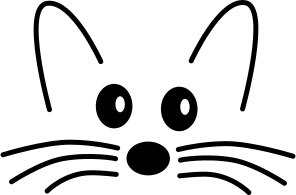
\includegraphics[width=1.4em]{squeak-logo}}}
\newcommand{\dothis}[1]{%
	\medskip
	\noindent\dothisicon
	\ifx#1\empty\else\quad\emph{#1}\fi
	\par\smallskip\nopagebreak}
% NB: To use this in an individual chapter, you must set:
%\graphicspath{{figures/} {../figures/}}
% at the head of the chapter.  Don't forget the final /
%=============================================================
%:Reader hints (hint)
%
% Indicates a non-obvious consequence 
\newcommand{\hint}[1]{\vspace{1ex}\noindent\fbox{\textsc{Astuce}} \emph{#1}}
%=================================================================
% graphics for Morphic handles
\newcommand{\grabHandle}{\raisebox{-0.2ex}{
\includegraphics[width=1em]{blackHandle}}}
\newcommand{\moveHandle}{\raisebox{-0.2ex}{
\includegraphics[width=1em]{moveHandle}}}
\newcommand{\debugHandle}{\raisebox{-0.2ex}{
\includegraphics[width=1em]{debugHandle}}}
% squeak-fr (added for Morphic handles)
\newcommand{\rotateHandle}{\raisebox{-0.2ex}{
\includegraphics[width=1em]{rotateHandle}}}
\newcommand{\viewerHandle}{\raisebox{-0.2ex}{
\includegraphics[width=1em]{viewerHandle}}}
% squeak-fr (add cloverHandle to use \clover in QuickTour.tex as alias
% todo 

%=============================================================
%:Highlighting Important stuff (doublebox)
%
% From Seaside book ...
\newsavebox{\SavedText}
\newlength{\InnerBoxRule}\setlength{\InnerBoxRule}{.75\fboxrule}
\newlength{\OuterBoxRule}\setlength{\OuterBoxRule}{1.5\fboxrule}
\newlength{\BoxSeparation}\setlength{\BoxSeparation}{1.5\fboxrule}
\addtolength{\BoxSeparation}{.5pt}
\newlength{\SaveBoxSep}\setlength{\SaveBoxSep}{2\fboxsep}
%
\newenvironment{doublebox}{\begin{lrbox}{\SavedText}
    \begin{minipage}{.75\textwidth}}
    {\end{minipage}\end{lrbox}\begin{center}
    \setlength{\fboxsep}{\BoxSeparation}\setlength{\fboxrule}{\OuterBoxRule}
    \fbox{\setlength{\fboxsep}{\SaveBoxSep}\setlength{\fboxrule}{\InnerBoxRule}%
      \fbox{\usebox{\SavedText}}}
  \end{center}}
% Use this:
%\newcommand{\important}[1]{\begin{doublebox}#1\end{doublebox}}


\newcommand{\important}[1]{
\noindent\rule{\textwidth}{2pt}\par
\textbf{Important!} #1 \par
\noindent\rule{\textwidth}{2pt}}

\newcommand{\note}[1]{
\noindent\rule{\textwidth}{2pt}\par
\noindent\textbf{Note} #1\par
\noindent\rule{\textwidth}{2pt}}

%=============================================================
%:Section depth
\setcounter{secnumdepth}{2}
%% for this to happen start the file with
%\ifx\wholebook\relax\else
%% $Author$ Martial
% $Date$ Wed Oct 10 13:34:55 CEST 2007
% $Revision$ source: SBE 12715 
% Last Changed Date: 2007-10-08 21:32:45 +0200 (Mon, 08 Oct 2007)
%=============================================================
% NB: documentclass must be set in main document.
% Allows book to be generated in multiple formats.
%=============================================================
%:Packages
%\usepackage[french]{babel}
\usepackage[T1]{fontenc}  %%%%%% really important to get the code directly in the text!
\usepackage{lmodern}
%\usepackage[scaled=0.85]{bookmanx} % needs another scale factor if used with \renewcommand{\sfdefault}{cmbr}
\usepackage{palatino}
%\usepackage[sc]{mathpazo}
%\linespread{1.05}
\usepackage[scaled=0.85]{helvet}
\usepackage{microtype}
\usepackage{graphicx}
\usepackage{theorem}
\usepackage[utf8]{inputenc}
% ON: pdfsync breaks the use of p{width} for tabular columns!
\ifdefined\usepdfsync\usepackage{pdfsync}\fi % Requires texlive 2007
%=============================================================
%:More packages
%Stef should check which ones are used!
%\usepackage{picinpar}
%\usepackage{layout}
%\usepackage{color}
%\definecolor{stefgris}{rgb}{0.85,0.85,0.85}
%\usepackage{enum}
%\usepackage{a4wide}
% \usepackage{fancyhdr}
\usepackage{ifthen}
\usepackage{float}
\usepackage{longtable}
\usepackage{makeidx}
\usepackage[nottoc]{tocbibind}
\usepackage{multicol}
\usepackage{booktabs}	% book-style tables
\usepackage{topcapt}	% enables \topcaption
\usepackage{multirow}
\usepackage{tabularx}
%\usepackage[bottom]{footmisc}
\usepackage{xspace}
\usepackage{alltt}
\usepackage{amssymb,textcomp}
\usepackage[usenames,dvipsnames]{color}
\usepackage{colortbl}
\usepackage[hang]{subfigure}\makeatletter\def\p@subfigure{\thefigure\,}\makeatother
\usepackage{rotating}
\usepackage{enumitem}	% apb: allows more control over tags in enumerations
\usepackage{verbatim}     % for comment environment
\usepackage{varioref}	% for page references that work
\labelformat{footnote}{\thechapter--#1} % to distinguish citations from jurabib
\usepackage{needspace}
\usepackage{isodateo} % enable \isodate
\usepackage[newparttoc]{titlesec}
\usepackage{titletoc}
\usepackage{eurosym}
\usepackage{wrapfig}

\usepackage[
	super,
	citefull=first,
	authorformat={allreversed,and},
	titleformat={commasep,italic}
]{jurabib} % citations as footnotes
\usepackage[
	colorlinks=true,
	linkcolor=black,
	urlcolor=black,
	citecolor=black
]{hyperref}   % should come last

%=============================================================
%:URL style
\makeatletter

\def\url@leostyle{%
  \@ifundefined{selectfont}{\def\UrlFont{\sf}}{\def\UrlFont{\sffamily}}}
% ajouter par Martial pour \traduit (met une dague dans les \doublebox
\def\thempfootnote{\fnsymbol{mpfootnote}}

\makeatother
% Now actually use the newly defined style.
\urlstyle{leo}
%=============================================================
%:Booleans
\newboolean{lulu}
\setboolean{lulu}{false}
\newcommand{\ifluluelse}[2]{\ifthenelse{\boolean{lulu}}{#1}{#2}}
%=============================================================
%:Names
\newcommand{\SUnit}{SUnit\xspace}
\newcommand{\sunit}{SUnit\xspace}
\newcommand{\xUnit}{$x$Unit\xspace}
\newcommand{\JUnit}{JUnit\xspace}
%\newcommand{\XP}{eXtreme Programming\xspace}
\newcommand{\st}{Smalltalk\xspace}
\newcommand{\Squeak}{Squeak\xspace}
\newcommand{\sq}{Squeak\xspace}
\newcommand{\sqmap}{SqueakMap\xspace}
\newcommand{\squeak}{Squeak\xspace}
%\newcommand{\sbe}{\url{scg.unibe.ch/SBE}\xspace}
%\newcommand{\sbe}{\url{squeakbyexample.org}\xspace}
\newcommand{\sbe}{\url{SqueakByExample.org}\xspace}
% squeak-fr: adresse de la version francaise
\newcommand{\spe}{\url{SqueakByExample.org/fr}\xspace}
\newcommand{\sba}{\url{SquareBracketAssociates.org}\xspace}

% squeak-fr: ajout de la \squeakdev pour eviter les problemes de
% changements d'url rencontres dans la VO:
\newcommand{\squeakdev}{\url{www.squeaksource.com/ImageForDevelopers}\xspace} %ou
%\newcommand{\squeakdev}{\url{squeak.ofset.org/squeak-dev}\xspace}

%=============================================================
%:Editorial comment macros
\newcommand{\nnbb}[2]{
    \fbox{\bfseries\sffamily\scriptsize#1}
    {\sf\small$\blacktriangleright$\textit{#2}$\blacktriangleleft$}
   }
\newcommand{\ab}[1]{\nnbb{Andrew}{#1}}
\newcommand{\sd}[1]{\nnbb{St\'{e}f}{#1}}
\newcommand{\md}[1]{\nnbb{Marcus}{#1}}
\newcommand{\on}[1]{\nnbb{Oscar}{#1}}
\newcommand{\damien}[1]{\nnbb{Damien}{#1}}
\newcommand{\lr}[1]{\nnbb{Lukas}{#1}}
\newcommand{\orla}[1]{\nnbb{Orla}{#1}}
%\newcommand{\here}{\nnbb{CONTINUE}{HERE}}
\newcommand{\here}{\nnbb{CONTINUE}{ICI}}

%=============================================================
%:Abbreviation macros
\newcommand{\ie}{\emph{c-\`a-d.}\xspace}
\newcommand{\cad}{\emph{c-\`a-d.}\xspace}
%\newcommand{\eg}{\emph{e.g.},\xspace}
\newcommand{\eg}{\emph{par ex.},\xspace}
\newcommand{\parex}{\emph{par ex.},\xspace}
\newcommand{\etc}{etc\xspace}
%=============================================================
%:Cross reference macros

% [squeak-fr] martial: remarquez les articles devant les noms
\newcommand{\charef}[1]{le chapitre~\ref{cha:#1}\xspace}
% note de martial: utilise dans chapitre Syntax.tex: a redefinir
\newcommand{\charefs}[2]{les chapitres~\ref{cha:#1} et \ref{cha:#2}\xspace}
\newcommand{\secref}[1]{la section~\ref{sec:#1}\xspace}
\newcommand{\figref}[1]{la figure~\ref{fig:#1}\xspace}
\newcommand{\Figref}[1]{La figure~\ref{fig:#1}\xspace}
\newcommand{\appref}[1]{l'annexe~\ref{app:#1}\xspace}
\newcommand{\tabref}[1]{la table~\ref{tab:#1}\xspace}
% defini pour le chapitre Messages.tex
\newcommand{\Tabref}[1]{La table~\ref{tab:#1}\xspace}

% APB: I removed trailing \xspace commands from these macros because
% \xspace mostly doesn't work.  If you want a space after your
% references, type one!
% ON: xspace has always worked just fine for me!  Please leave them in.
%
\newcommand{\ruleref}[1]{\ref{rule:#1}\xspace}
%
\newcommand{\egref}[1]{exemple~\ref{eg:#1}\xspace}
\newcommand{\Egref}[1]{Exemple~\ref{eg:#1}\xspace}
%
\newcommand{\scrref}[1]{script~\ref{scr:#1}\xspace}
\newcommand{\Scrref}[1]{Script~\ref{scr:#1}\xspace}
% t = the
\newcommand{\tscrref}[1]{le script~\ref{scr:#1}\xspace}
\newcommand{\Tscrref}[1]{Le script~\ref{scr:#1}\xspace}
%
\newcommand{\mthref}[1]{m\'ethode~\ref{mth:#1}\xspace}
\newcommand{\mthsref}[1]{m\'ethodes~\ref{mth:#1}\xspace}
\newcommand{\Mthref}[1]{M\'ethode~\ref{mth:#1}\xspace}
\newcommand{\tmthref}[1]{la m\'ethode~\ref{mth:#1}\xspace}
\newcommand{\Tmthref}[1]{La m\'ethode~\ref{mth:#1}\xspace}
%
\newcommand{\clsref}[1]{classe~\ref{cls:#1}\xspace}
\newcommand{\tclsref}[1]{la classe~\ref{cls:#1}\xspace}
\newcommand{\Tclsref}[1]{La classe~\ref{cls:#1}\xspace}
%=============================================================
%:Menu item macro
% for menu items, so we can change our minds on how to print them! (apb)
\definecolor{lightgray}{gray}{0.89}
\newcommand{\menu}[1]{{%
	\setlength{\fboxsep}{0pt}%
	\colorbox{lightgray}{{{\upshape\sffamily\strut \,#1\,}}}}}
% \newcommand{\menu}[1]{{%
% 	\fontfamily{lmr}\selectfont
% 	\upshape\textlangle{\sffamily #1}\textrangle}}
% For submenu items:
\newcommand{\go}{\,$\triangleright$\,}
% \newcommand{\go}{\,$\blacktriangleright$\,}
% For keyboard shortcuts:
%\newcommand{\short}[1]{\mbox{$\langle${\sc CMD}$\rangle$-#1}\xspace}
\newcommand{\short}[1]{\mbox{{\sc cmd}\hspace{0.08em}--\hspace{0.09em}#1}\xspace}
% For buttons:
\newcommand{\button}[1]{{%
	\setlength{\fboxsep}{0pt}%
	\fbox{{\upshape\sffamily\strut \,#1\,}}}}
\newcommand{\toolsflap}{l'onglet \textit{Tools}\xspace}
%=============================================================
%:Reader cues (do this)
%
% Indicate something the reader should try out.
\newcommand{\dothisicon}{\raisebox{-.5ex}{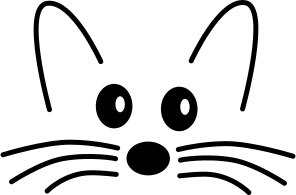
\includegraphics[width=1.4em]{squeak-logo}}}
\newcommand{\dothis}[1]{%
	\medskip
	\noindent\dothisicon
	\ifx#1\empty\else\quad\emph{#1}\fi
	\par\smallskip\nopagebreak}
% NB: To use this in an individual chapter, you must set:
%\graphicspath{{figures/} {../figures/}}
% at the head of the chapter.  Don't forget the final /
%=============================================================
%:Reader hints (hint)
%
% Indicates a non-obvious consequence 
\newcommand{\hint}[1]{\vspace{1ex}\noindent\fbox{\textsc{Astuce}} \emph{#1}}
%=================================================================
% graphics for Morphic handles
\newcommand{\grabHandle}{\raisebox{-0.2ex}{
\includegraphics[width=1em]{blackHandle}}}
\newcommand{\moveHandle}{\raisebox{-0.2ex}{
\includegraphics[width=1em]{moveHandle}}}
\newcommand{\debugHandle}{\raisebox{-0.2ex}{
\includegraphics[width=1em]{debugHandle}}}
% squeak-fr (added for Morphic handles)
\newcommand{\rotateHandle}{\raisebox{-0.2ex}{
\includegraphics[width=1em]{rotateHandle}}}
\newcommand{\viewerHandle}{\raisebox{-0.2ex}{
\includegraphics[width=1em]{viewerHandle}}}
% squeak-fr (add cloverHandle to use \clover in QuickTour.tex as alias
% todo 

%=============================================================
%:Highlighting Important stuff (doublebox)
%
% From Seaside book ...
\newsavebox{\SavedText}
\newlength{\InnerBoxRule}\setlength{\InnerBoxRule}{.75\fboxrule}
\newlength{\OuterBoxRule}\setlength{\OuterBoxRule}{1.5\fboxrule}
\newlength{\BoxSeparation}\setlength{\BoxSeparation}{1.5\fboxrule}
\addtolength{\BoxSeparation}{.5pt}
\newlength{\SaveBoxSep}\setlength{\SaveBoxSep}{2\fboxsep}
%
\newenvironment{doublebox}{\begin{lrbox}{\SavedText}
    \begin{minipage}{.75\textwidth}}
    {\end{minipage}\end{lrbox}\begin{center}
    \setlength{\fboxsep}{\BoxSeparation}\setlength{\fboxrule}{\OuterBoxRule}
    \fbox{\setlength{\fboxsep}{\SaveBoxSep}\setlength{\fboxrule}{\InnerBoxRule}%
      \fbox{\usebox{\SavedText}}}
  \end{center}}
% Use this:
%\newcommand{\important}[1]{\begin{doublebox}#1\end{doublebox}}


\newcommand{\important}[1]{
\noindent\rule{\textwidth}{2pt}\par
\textbf{Important!} #1 \par
\noindent\rule{\textwidth}{2pt}}

\newcommand{\note}[1]{
\noindent\rule{\textwidth}{2pt}\par
\noindent\textbf{Note} #1\par
\noindent\rule{\textwidth}{2pt}}

%=============================================================
%:Section depth
\setcounter{secnumdepth}{2}
%% for this to happen start the file with
%\ifx\wholebook\relax\else
%% $Author$ Martial
% $Date$ Wed Oct 10 13:34:55 CEST 2007
% $Revision$ source: SBE 12715 
% Last Changed Date: 2007-10-08 21:32:45 +0200 (Mon, 08 Oct 2007)
%=============================================================
% NB: documentclass must be set in main document.
% Allows book to be generated in multiple formats.
%=============================================================
%:Packages
%\usepackage[french]{babel}
\usepackage[T1]{fontenc}  %%%%%% really important to get the code directly in the text!
\usepackage{lmodern}
%\usepackage[scaled=0.85]{bookmanx} % needs another scale factor if used with \renewcommand{\sfdefault}{cmbr}
\usepackage{palatino}
%\usepackage[sc]{mathpazo}
%\linespread{1.05}
\usepackage[scaled=0.85]{helvet}
\usepackage{microtype}
\usepackage{graphicx}
\usepackage{theorem}
\usepackage[utf8]{inputenc}
% ON: pdfsync breaks the use of p{width} for tabular columns!
\ifdefined\usepdfsync\usepackage{pdfsync}\fi % Requires texlive 2007
%=============================================================
%:More packages
%Stef should check which ones are used!
%\usepackage{picinpar}
%\usepackage{layout}
%\usepackage{color}
%\definecolor{stefgris}{rgb}{0.85,0.85,0.85}
%\usepackage{enum}
%\usepackage{a4wide}
% \usepackage{fancyhdr}
\usepackage{ifthen}
\usepackage{float}
\usepackage{longtable}
\usepackage{makeidx}
\usepackage[nottoc]{tocbibind}
\usepackage{multicol}
\usepackage{booktabs}	% book-style tables
\usepackage{topcapt}	% enables \topcaption
\usepackage{multirow}
\usepackage{tabularx}
%\usepackage[bottom]{footmisc}
\usepackage{xspace}
\usepackage{alltt}
\usepackage{amssymb,textcomp}
\usepackage[usenames,dvipsnames]{color}
\usepackage{colortbl}
\usepackage[hang]{subfigure}\makeatletter\def\p@subfigure{\thefigure\,}\makeatother
\usepackage{rotating}
\usepackage{enumitem}	% apb: allows more control over tags in enumerations
\usepackage{verbatim}     % for comment environment
\usepackage{varioref}	% for page references that work
\labelformat{footnote}{\thechapter--#1} % to distinguish citations from jurabib
\usepackage{needspace}
\usepackage{isodateo} % enable \isodate
\usepackage[newparttoc]{titlesec}
\usepackage{titletoc}
\usepackage{eurosym}
\usepackage{wrapfig}

\usepackage[
	super,
	citefull=first,
	authorformat={allreversed,and},
	titleformat={commasep,italic}
]{jurabib} % citations as footnotes
\usepackage[
	colorlinks=true,
	linkcolor=black,
	urlcolor=black,
	citecolor=black
]{hyperref}   % should come last

%=============================================================
%:URL style
\makeatletter

\def\url@leostyle{%
  \@ifundefined{selectfont}{\def\UrlFont{\sf}}{\def\UrlFont{\sffamily}}}
% ajouter par Martial pour \traduit (met une dague dans les \doublebox
\def\thempfootnote{\fnsymbol{mpfootnote}}

\makeatother
% Now actually use the newly defined style.
\urlstyle{leo}
%=============================================================
%:Booleans
\newboolean{lulu}
\setboolean{lulu}{false}
\newcommand{\ifluluelse}[2]{\ifthenelse{\boolean{lulu}}{#1}{#2}}
%=============================================================
%:Names
\newcommand{\SUnit}{SUnit\xspace}
\newcommand{\sunit}{SUnit\xspace}
\newcommand{\xUnit}{$x$Unit\xspace}
\newcommand{\JUnit}{JUnit\xspace}
%\newcommand{\XP}{eXtreme Programming\xspace}
\newcommand{\st}{Smalltalk\xspace}
\newcommand{\Squeak}{Squeak\xspace}
\newcommand{\sq}{Squeak\xspace}
\newcommand{\sqmap}{SqueakMap\xspace}
\newcommand{\squeak}{Squeak\xspace}
%\newcommand{\sbe}{\url{scg.unibe.ch/SBE}\xspace}
%\newcommand{\sbe}{\url{squeakbyexample.org}\xspace}
\newcommand{\sbe}{\url{SqueakByExample.org}\xspace}
% squeak-fr: adresse de la version francaise
\newcommand{\spe}{\url{SqueakByExample.org/fr}\xspace}
\newcommand{\sba}{\url{SquareBracketAssociates.org}\xspace}

% squeak-fr: ajout de la \squeakdev pour eviter les problemes de
% changements d'url rencontres dans la VO:
\newcommand{\squeakdev}{\url{www.squeaksource.com/ImageForDevelopers}\xspace} %ou
%\newcommand{\squeakdev}{\url{squeak.ofset.org/squeak-dev}\xspace}

%=============================================================
%:Editorial comment macros
\newcommand{\nnbb}[2]{
    \fbox{\bfseries\sffamily\scriptsize#1}
    {\sf\small$\blacktriangleright$\textit{#2}$\blacktriangleleft$}
   }
\newcommand{\ab}[1]{\nnbb{Andrew}{#1}}
\newcommand{\sd}[1]{\nnbb{St\'{e}f}{#1}}
\newcommand{\md}[1]{\nnbb{Marcus}{#1}}
\newcommand{\on}[1]{\nnbb{Oscar}{#1}}
\newcommand{\damien}[1]{\nnbb{Damien}{#1}}
\newcommand{\lr}[1]{\nnbb{Lukas}{#1}}
\newcommand{\orla}[1]{\nnbb{Orla}{#1}}
%\newcommand{\here}{\nnbb{CONTINUE}{HERE}}
\newcommand{\here}{\nnbb{CONTINUE}{ICI}}

%=============================================================
%:Abbreviation macros
\newcommand{\ie}{\emph{c-\`a-d.}\xspace}
\newcommand{\cad}{\emph{c-\`a-d.}\xspace}
%\newcommand{\eg}{\emph{e.g.},\xspace}
\newcommand{\eg}{\emph{par ex.},\xspace}
\newcommand{\parex}{\emph{par ex.},\xspace}
\newcommand{\etc}{etc\xspace}
%=============================================================
%:Cross reference macros

% [squeak-fr] martial: remarquez les articles devant les noms
\newcommand{\charef}[1]{le chapitre~\ref{cha:#1}\xspace}
% note de martial: utilise dans chapitre Syntax.tex: a redefinir
\newcommand{\charefs}[2]{les chapitres~\ref{cha:#1} et \ref{cha:#2}\xspace}
\newcommand{\secref}[1]{la section~\ref{sec:#1}\xspace}
\newcommand{\figref}[1]{la figure~\ref{fig:#1}\xspace}
\newcommand{\Figref}[1]{La figure~\ref{fig:#1}\xspace}
\newcommand{\appref}[1]{l'annexe~\ref{app:#1}\xspace}
\newcommand{\tabref}[1]{la table~\ref{tab:#1}\xspace}
% defini pour le chapitre Messages.tex
\newcommand{\Tabref}[1]{La table~\ref{tab:#1}\xspace}

% APB: I removed trailing \xspace commands from these macros because
% \xspace mostly doesn't work.  If you want a space after your
% references, type one!
% ON: xspace has always worked just fine for me!  Please leave them in.
%
\newcommand{\ruleref}[1]{\ref{rule:#1}\xspace}
%
\newcommand{\egref}[1]{exemple~\ref{eg:#1}\xspace}
\newcommand{\Egref}[1]{Exemple~\ref{eg:#1}\xspace}
%
\newcommand{\scrref}[1]{script~\ref{scr:#1}\xspace}
\newcommand{\Scrref}[1]{Script~\ref{scr:#1}\xspace}
% t = the
\newcommand{\tscrref}[1]{le script~\ref{scr:#1}\xspace}
\newcommand{\Tscrref}[1]{Le script~\ref{scr:#1}\xspace}
%
\newcommand{\mthref}[1]{m\'ethode~\ref{mth:#1}\xspace}
\newcommand{\mthsref}[1]{m\'ethodes~\ref{mth:#1}\xspace}
\newcommand{\Mthref}[1]{M\'ethode~\ref{mth:#1}\xspace}
\newcommand{\tmthref}[1]{la m\'ethode~\ref{mth:#1}\xspace}
\newcommand{\Tmthref}[1]{La m\'ethode~\ref{mth:#1}\xspace}
%
\newcommand{\clsref}[1]{classe~\ref{cls:#1}\xspace}
\newcommand{\tclsref}[1]{la classe~\ref{cls:#1}\xspace}
\newcommand{\Tclsref}[1]{La classe~\ref{cls:#1}\xspace}
%=============================================================
%:Menu item macro
% for menu items, so we can change our minds on how to print them! (apb)
\definecolor{lightgray}{gray}{0.89}
\newcommand{\menu}[1]{{%
	\setlength{\fboxsep}{0pt}%
	\colorbox{lightgray}{{{\upshape\sffamily\strut \,#1\,}}}}}
% \newcommand{\menu}[1]{{%
% 	\fontfamily{lmr}\selectfont
% 	\upshape\textlangle{\sffamily #1}\textrangle}}
% For submenu items:
\newcommand{\go}{\,$\triangleright$\,}
% \newcommand{\go}{\,$\blacktriangleright$\,}
% For keyboard shortcuts:
%\newcommand{\short}[1]{\mbox{$\langle${\sc CMD}$\rangle$-#1}\xspace}
\newcommand{\short}[1]{\mbox{{\sc cmd}\hspace{0.08em}--\hspace{0.09em}#1}\xspace}
% For buttons:
\newcommand{\button}[1]{{%
	\setlength{\fboxsep}{0pt}%
	\fbox{{\upshape\sffamily\strut \,#1\,}}}}
\newcommand{\toolsflap}{l'onglet \textit{Tools}\xspace}
%=============================================================
%:Reader cues (do this)
%
% Indicate something the reader should try out.
\newcommand{\dothisicon}{\raisebox{-.5ex}{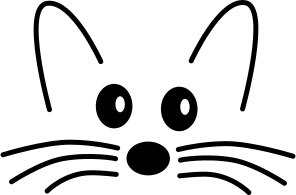
\includegraphics[width=1.4em]{squeak-logo}}}
\newcommand{\dothis}[1]{%
	\medskip
	\noindent\dothisicon
	\ifx#1\empty\else\quad\emph{#1}\fi
	\par\smallskip\nopagebreak}
% NB: To use this in an individual chapter, you must set:
%\graphicspath{{figures/} {../figures/}}
% at the head of the chapter.  Don't forget the final /
%=============================================================
%:Reader hints (hint)
%
% Indicates a non-obvious consequence 
\newcommand{\hint}[1]{\vspace{1ex}\noindent\fbox{\textsc{Astuce}} \emph{#1}}
%=================================================================
% graphics for Morphic handles
\newcommand{\grabHandle}{\raisebox{-0.2ex}{
\includegraphics[width=1em]{blackHandle}}}
\newcommand{\moveHandle}{\raisebox{-0.2ex}{
\includegraphics[width=1em]{moveHandle}}}
\newcommand{\debugHandle}{\raisebox{-0.2ex}{
\includegraphics[width=1em]{debugHandle}}}
% squeak-fr (added for Morphic handles)
\newcommand{\rotateHandle}{\raisebox{-0.2ex}{
\includegraphics[width=1em]{rotateHandle}}}
\newcommand{\viewerHandle}{\raisebox{-0.2ex}{
\includegraphics[width=1em]{viewerHandle}}}
% squeak-fr (add cloverHandle to use \clover in QuickTour.tex as alias
% todo 

%=============================================================
%:Highlighting Important stuff (doublebox)
%
% From Seaside book ...
\newsavebox{\SavedText}
\newlength{\InnerBoxRule}\setlength{\InnerBoxRule}{.75\fboxrule}
\newlength{\OuterBoxRule}\setlength{\OuterBoxRule}{1.5\fboxrule}
\newlength{\BoxSeparation}\setlength{\BoxSeparation}{1.5\fboxrule}
\addtolength{\BoxSeparation}{.5pt}
\newlength{\SaveBoxSep}\setlength{\SaveBoxSep}{2\fboxsep}
%
\newenvironment{doublebox}{\begin{lrbox}{\SavedText}
    \begin{minipage}{.75\textwidth}}
    {\end{minipage}\end{lrbox}\begin{center}
    \setlength{\fboxsep}{\BoxSeparation}\setlength{\fboxrule}{\OuterBoxRule}
    \fbox{\setlength{\fboxsep}{\SaveBoxSep}\setlength{\fboxrule}{\InnerBoxRule}%
      \fbox{\usebox{\SavedText}}}
  \end{center}}
% Use this:
%\newcommand{\important}[1]{\begin{doublebox}#1\end{doublebox}}


\newcommand{\important}[1]{
\noindent\rule{\textwidth}{2pt}\par
\textbf{Important!} #1 \par
\noindent\rule{\textwidth}{2pt}}

\newcommand{\note}[1]{
\noindent\rule{\textwidth}{2pt}\par
\noindent\textbf{Note} #1\par
\noindent\rule{\textwidth}{2pt}}

%=============================================================
%:Section depth
\setcounter{secnumdepth}{2}
%% for this to happen start the file with
%\ifx\wholebook\relax\else
%\input{../common.tex}
%\begin{document}
%\fi
% and terminate by
% \ifx\wholebook\relax\else\end{document}\fi

\DeclareGraphicsExtensions{.pdf, .jpg, .png}
%=============================================================
%:PDF setup
\hypersetup{
%   a4paper,
%   pdfstartview=FitV,
%   colorlinks,
%   linkcolor=darkblue,
%   citecolor=darkblue,
%   pdftitle={Squeak by Example},
pdftitle={Squeak par l'exemple},
   pdfauthor={Andrew Black, St\'ephane Ducasse,	Oscar Nierstrasz,
Damien Pollet},
   pdfkeywords={Smalltalk, Squeak, Programmation Orient\'ee Objet},
pdfsubject={Informatique, Computer Science}
}
%=============================================================
%:Page layout and appearance
%
% \renewcommand{\headrulewidth}{0pt}
\renewcommand{\chaptermark}[1]{\markboth{#1}{}}
\renewcommand{\sectionmark}[1]{\markright{\thesection\ #1}}
\renewpagestyle{plain}[\small\itshape]{%
	\setheadrule{0pt}%
	\sethead[][][]{}{}{}%
	\setfoot[][][]{}{}{}}
\renewpagestyle{headings}[\small\itshape]{%
	\setheadrule{0pt}%
	\setmarks{chapter}{section}%
	\sethead[\thepage][][\chaptertitle]{\sectiontitle}{}{\thepage}%
	\setfoot[][][]{}{}{}}
% pagestyle for tableofcontents + index (martial: 2008/04/23)
\newpagestyle{newheadings}[\small\itshape]{%
	\setheadrule{0pt}%
	\setmarks{chapter}{section}%
	\sethead[\thepage][][\chaptertitle]{\chaptertitle}{}{\thepage}%
	\setfoot[][][]{}{}{}}
%=============================================================
%:Title section setup and TOC numbering depth
\setcounter{secnumdepth}{1}
\setcounter{tocdepth}{1}
\titleformat{\part}[display]{\centering}{\huge\partname\ \thepart}{1em}{\Huge\textbf}[]
\titleformat{\chapter}[display]{}{\huge\chaptertitlename\ \thechapter}{1em}{\Huge\raggedright\textbf}[]
\titlecontents{part}[3pc]{%
		\pagebreak[2]\addvspace{1em plus.4em minus.2em}%
		\leavevmode\large\bfseries}
	{\contentslabel{3pc}}{\hspace*{-3pc}}
	{}[\nopagebreak]
\titlecontents{chapter}[3pc]{%
		\pagebreak[0]\addvspace{1em plus.2em minus.2em}%
		\leavevmode\bfseries}
	{\contentslabel{3pc}}{}
	{\hfill\contentspage}[\nopagebreak]
\dottedcontents{section}[3pc]{}{3pc}{1pc}
\dottedcontents{subsection}[3pc]{}{0pc}{1pc}
% \dottedcontents{subsection}[4.5em]{}{0pt}{1pc}
% Make \cleardoublepage insert really blank pages http://www.tex.ac.uk/cgi-bin/texfaq2html?label=reallyblank
\let\origdoublepage\cleardoublepage
\newcommand{\clearemptydoublepage}{%
  \clearpage
  {\pagestyle{empty}\origdoublepage}}
\let\cleardoublepage\clearemptydoublepage % see http://www.tex.ac.uk/cgi-bin/texfaq2html?label=patch
%=============================================================
%:FAQ macros (for FAQ chapter)
\newtheorem{faq}{FAQ}
\newcommand{\answer}{\paragraph{R\'eponse}\ }
%=============================================================
%:Listings package configuration
\usepackage{listings}
\newcommand{\caret}{\makebox{\raisebox{0.4ex}{\footnotesize{$\wedge$}}}}
\lstdefinelanguage{Smalltalk}{
%  morekeywords={self,super,true,false,nil,thisContext}, % This is overkill
  morestring=[d]',
  morecomment=[s]{"}{"},
  alsoletter={\#:},
  escapechar={!},
  escapebegin=\itshape, % comment-like by default (Martial 11/2007)
  literate=
    {BANG}{!}1
    {UNDERSCORE}{\_}1
    {\\st}{Smalltalk}9 % convenience -- in case \st occurs in code
    % {'}{{\textquotesingle}}1 % replaced by upquote=true in \lstset
    {_}{{$\leftarrow$}}1
    {>>>}{{\sep}}1
    {^}{{$\uparrow$}}1
    {~}{{$\sim$}}1
    {-}{{\sf -\hspace{-0.13em}-}}1  % the goal is to make - the same width as +
    {+}{\raisebox{0.08ex}{+}}1		% and to raise + off the baseline to match -
    {-->}{{\quad$\longrightarrow$\quad}}3
	, % Don't forget the comma at the end!
  tabsize=4
}[keywords,comments,strings]
% ajout pour les échappements dans les codes
% indispensable pour mettre le code en emphase (cf. Model.tex) 
\newcommand{\codeify}[1]{\NoAutoSpaceBeforeFDP#1\AutoSpaceBeforeFDP}
\newcommand{\normcomment}[1]{\emph{#1}} %cf. Streams
\newcommand{\normcode}[1]{\emph{\codeify{#1}}} %cf. Streams
\newcommand{\emcode}[1]{\textbf{\normcode{#1}}} % Martial 11/2007
\lstset{language=Smalltalk,
	basicstyle=\sffamily,
	keywordstyle=\color{black}\bfseries,
	% stringstyle=\ttfamily, % Ugly! do we really want this? -- on
	%commentstyle=\itshape,
	mathescape=true,
	showstringspaces=false,
	keepspaces=true,
	breaklines=true,
	breakautoindent=true,
	lineskip={-1pt}, % Ugly hack
	upquote=true, % straight quote; requires textcomp package
	columns=fullflexible} % no fixed width fonts
% In-line code (literal)
% Normally use this for all in-line code:
\newcommand{\ct}{\lstinline[mathescape=false,basicstyle={\sffamily\upshape}]}
% apb 2007.8.28 added the \upshape declaration to avoid getting italicized code in \dothis{ } sections.
% In-line code (latex enabled)
% Use this only in special situations where \ct does not work
% (within section headings ...):

% [squeak-fr] Modification de \lct suivant les indications de Martial Boniou
\newcommand{\lct}[1]{\textsf{\textup{\NoAutoSpaceBeforeFDP #1
\AutoSpaceBeforeFDP}}} %\xspace

% Use these for system categories and protocols:
\newcommand{\scat}[1]{\emph{\textsf{#1}}\xspace}
\newcommand{\pkg}[1]{\emph{\textsf{#1}}\xspace}
\newcommand{\prot}[1]{\emph{\textsf{#1}}\xspace}
% Code environments
% NB: the arg is for tests
% Only code and example environments may be tests
\lstnewenvironment{code}[1]{%
	\lstset{%
		frame=lines,
		mathescape=false
	}
}{}
\def\ignoredollar#1{}
%=============================================================
%:Code environments (method, script ...)
% NB: the third arg is for tests
% Only code and example environments may be tests
\lstnewenvironment{example}[3][defaultlabel]{%
	\renewcommand{\lstlistingname}{Exemple}%
	\lstset{
		frame=lines,
		mathescape=false,
		caption={\emph{#2}},
		label={eg:#1}
	}
}{}
\lstnewenvironment{script}[2][defaultlabel]{%
\renewcommand{\lstlistingname}{Script}%
	\lstset{
		frame=lines,
		mathescape=false,
		name={Script},
		caption={\emph{#2}},
		label={scr:#1}
	}
}{}
%I could not find a way yo get the Experiment #numb followed by the caption in a black box
%\colorbox{black}{\makebox[\textwidth]{  \color{white} {\large {\bfseries Experiment 3-1 (crear i moure un robot)}} }}
\lstnewenvironment{experiment}[2][defaultlabel]{%
%\noindent\rule{\textwidth}{2pt}\vspace{-0.8cm}
\renewcommand{\lstlistingname}{Experiment}%
	\lstset{
		frame=none,
		rulecolor=\color{black},
		mathescape=false,
		name={Experiment},
		caption={\emph{#2}},
		label={scr:#1}
	}
}{%\vspace{-0.5cm}\noindent\rule{\textwidth}{2pt}
}

\lstnewenvironment{method}[2][defaultlabel]{%
	\renewcommand{\lstlistingname}{Method}%
	\lstset{
		frame=lines,
		mathescape=false,
		name={M\'ethode},
		caption={\emph{#2}},
		label={mth:#1}
	}
}{}
\lstnewenvironment{methods}[2][defaultlabel]{% just for multiple methods at once
	\renewcommand{\lstlistingname}{Methods}%
	\lstset{
		frame=lines,
		mathescape=false,
		name={M\'ethode},
		caption={\emph{#2}},
		label={mth:#1}
	}
}{}
\lstnewenvironment{numMethod}[2][defaultlabel]{%
	\renewcommand{\lstlistingname}{Method}%
	\lstset{
		numbers=left,
		numberstyle={\tiny\sffamily},
		frame=lines,
		mathescape=false,
		name={M\'ethode},
		caption={\emph{#2}},
		label={mth:#1}
	}
}{}
% \lstnewenvironment{classdef}[2][defaultlabel]{%
% 	\renewcommand{\lstlistingname}{Classe}%
% 	\lstset{
% 		frame=lines,
% 		mathescape=false,
% 		name={Classe},
% 		caption={\emph{#2}},
% 		label={cls:#1}
% 	}
% }{}

%%%%%%%%%%%%%%%%%%%%%%%%%%%%%%%%%%%%%%%%%%%%%%%%%%%%%%%%%%%%%%%%%%%%%%%%%%%%%%%%%%%%%%%%%%%%%%%%%
%%From the original book latex template
%%%%%%%%%%%%%%%%%%%%%%%%%%%%%%%%%%%%%%%%%%%%%%%%%%%%%%%%%%%%%%%%%%%%%%%%%%%%%%%%%%%%%%%%%%%%%%%%%
\theoremstyle{break}
{\theorembodyfont{\rmfamily}\theoremstyle{break}
\newtheorem{privScript}{Script}[chapter]
%\newtheorem{privMethod}{Method}[chapter]
\newtheorem{privExercise}{Experiment}[chapter]}

% \theoremstyle{break}
% {\theorembodyfont{\rmfamily} \newtheorem{privMethod}{Method}[chapter]}

%class
\theoremstyle{break}
{\theorembodyfont{\rmfamily} \newtheorem{privClassDef}{Class}[chapter]}

%important
\theoremstyle{break}
{\theorembodyfont{\rmfamily} \newtheorem{privTemplate}{Important Messages}[chapter]}

% experiment
\newenvironment{exercise}
    {\begin{privExercise}\mbox{}\\}
    {\end{privExercise}}


%%% for figure
\newsavebox{\ScriptFigure}
\newlength{\ScriptWidth}
\newlength{\FigureWidth}

%%%%%%%%%%%%%%%%%%%%%%%%%%%%%%%%%%%%%%%%%%%%%%%%%%%%%%%%%%%%%%%%%%%%%%%%%%%%%%%%
\newenvironment{scriptfig}[3][0.6]
   {\setlength{\ScriptWidth}{\linewidth*\real{#1}}%
   \setlength{\FigureWidth}{\linewidth-(\linewidth*\real{#1})}%
   \savebox{\ScriptFigure}%
	{\parbox{\FigureWidth}{\includegraphics[width=0.98\FigureWidth]{#2}}}%
   \par\noindent\begin{minipage}{\linewidth}\hrule\vskip 0.2cm\begin{minipage}[c]{\ScriptWidth}%
   \begin{stefscript}[{\em #3}]\begin{alltt}\sffamily}
   {\end{alltt}\end{stefscript}\end{minipage}\hfill
   \usebox{\ScriptFigure}
   \vskip 1ex\hrule\end{minipage}\vskip 1ex\par}

%%%%%%%%%%%%%%%%%%%%%%%%%%%%%%%%%%%%%%%%%%%%%%%%%%%%%%%%%%%%%%%%%%%%%%%%%%%%%%%%
%% to be able to specify the complete set of values for includegraphics
%% may be will be changed but not the interface
\newenvironment{scriptfigwithsize}[3][0.6]
   {\setlength{\ScriptWidth}{\linewidth*\real{#1}}%
   \setlength{\FigureWidth}{\linewidth-(\linewidth*\real{#1})}%
   \savebox{\ScriptFigure}{\parbox{\FigureWidth}{\raggedleft{#2}}}%
   \par\noindent\begin{minipage}{\linewidth}\hrule\vskip 0.3cm\begin{minipage}[c]{\ScriptWidth}%
   \begin{stefscript}[{\em #3}]\begin{alltt}\sffamily}
   {\end{alltt}\end{stefscript}\end{minipage}\hfill
   \usebox{\ScriptFigure}
   \vskip 1ex\hrule\end{minipage}\vskip 1ex\par}

% \newenvironment{methodfig}[2][0.6]
%    {\setlength{\ScriptWidth}{\linewidth*\real{#1}}%
%    \setlength{\FigureWidth}{\linewidth-(\linewidth*\real{#1})}%
%    \savebox{\ScriptFigure}{\parbox{\FigureWidth}{\includegraphics[width=.98\FigureWidth]{#2}}}%
%    \par\noindent\rule{\linewidth}{1mm}
%    \\[-0.3cm]\noindent\rule{\linewidth}{0.1mm}
%    \noindent\begin{minipage}[c]{\ScriptWidth}\begin{privMethod}\begin{alltt}\sffamily}
%    {\end{alltt}\end{privMethod}\end{minipage}\hfill
%    \usebox{\ScriptFigure} \vskip 1ex\hrule\vskip 1ex\par}

% \newenvironment{method}
% {\par\noindent\begin{minipage}{\linewidth}\vspace{0.2cm}\begin{privMethod}\begin{nminipage}\vspace{-0.2cm}\rule{\linewidth}{1mm}\\[-0.6cm]\rule{\linewidth}{0.1mm}\end{nminipage}\hspace*{\scriptindent}\codesize\begin{nalltt}\vspace{-0.2cm}}
% {\end{nalltt}\normalsize\vspace{-0.1cm}\hrule\end{privMethod}\vspace{0.2cm}\end{minipage}}


% \newenvironment{classdef}
% {\par\noindent\begin{minipage}{\linewidth}\vspace{0.2cm}\begin{privClassDef}\begin{nminipage}\vspace{-0.2cm}\rule{\linewidth}{1mm}\\[-0.6cm]\rule{\linewidth}{0.1mm}\end{nminipage}\hspace*{\scriptindent}\codesize\begin{nalltt}\vspace{-0.2cm}}
% {\end{nalltt}\normalsize\vspace{-0.1cm}\hrule\end{privClassDef}\vspace{0.2cm}\end{minipage}}


% \newenvironment{template}
% {\par\noindent\begin{minipage}{\linewidth}\vspace{0.3cm}\begin{privTemplate}\begin{nminipage}\vspace{-0.4cm}\rule{\linewidth}{0.1mm}\end{nminipage}\hspace*{\scriptindent}\begin{nalltt}\vspace{-0.7cm}}
% {\end{nalltt}\vspace{-0.1cm}\hrule\end{privTemplate}\end{minipage}\vspace{0.3cm}}

\newenvironment{exofig}[2][0.7]
   {\setlength{\ScriptWidth}{\linewidth*\real{#1}}
   \setlength{\FigureWidth}{\linewidth-(\linewidth*\real{#1})}
   \savebox{\ScriptFigure}{\parbox{\FigureWidth}{\raggedleft{\includegraphics[width=.98\FigureWidth]{#2}}}}
   \par\noindent\begin{minipage}{\linewidth}\hrule\vskip 0.3cm\begin{minipage}[c]{\ScriptWidth}%
   \begin{privExercise}}
   {\end{privExercise}\end{minipage}\hfill
   \usebox{\ScriptFigure}
   \vskip 1ex\hrule\end{minipage}\vskip 1ex\par}

\newenvironment{exofigwithsize}[2][0.7]
   {\setlength{\ScriptWidth}{\linewidth*\real{#1}}
   \setlength{\FigureWidth}{\linewidth-(\linewidth*\real{#1})}
   \savebox{\ScriptFigure}{\parbox{\FigureWidth}{\raggedleft{#2}}}
   \par\noindent\begin{minipage}{\linewidth}\hrule\vskip 0.3cm\begin{minipage}[c]{\ScriptWidth}%
   \begin{privExercise}}
   {\end{privExercise}\end{minipage}\hfill\usebox{\ScriptFigure}
   \vskip 1ex\hrule\end{minipage}\vskip 1ex\par}

\newenvironment{exofigwithsizeandtitle}[3][0.7]
   {\setlength{\ScriptWidth}{\linewidth*\real{#1}}
   \setlength{\FigureWidth}{\linewidth-(\linewidth*\real{#1})}
   \savebox{\ScriptFigure}{\parbox{\FigureWidth}{\raggedleft{#2}}}
   \vskip 0.3cm\par\noindent\begin{minipage}{\linewidth}\hrule\vskip 0.1cm\begin{minipage}[c]{\ScriptWidth}%
   \begin{privExercise}[\em{#3}]}
   {\end{privExercise}\end{minipage}\hfill\usebox{\ScriptFigure}
   \vskip 1ex\hrule\end{minipage}\vskip 1ex\par}

\newenvironment{exofigwithtitle}[3][0.7]
   {\setlength{\ScriptWidth}{\linewidth*\real{#1}}
   \setlength{\FigureWidth}{\linewidth-(\linewidth*\real{#1})}
   \savebox{\ScriptFigure}{\parbox{\FigureWidth}{\raggedleft{\includegraphics[width=.98\FigureWidth]{#2}}}}
   \par\noindent\begin{minipage}{\linewidth}\hrule\vskip 0.3cm\begin{minipage}[c]{\ScriptWidth}%
   \begin{privExercise}[\em{#3}]}
   {\end{privExercise}\end{minipage}\hfill
   \usebox{\ScriptFigure}
   \vskip 1ex\hrule\end{minipage}\vskip 1ex\par}


\newenvironment{exonofigwithtitle}[3][0.7]
   {\setlength{\ScriptWidth}{\linewidth*\real{#1}}
   \setlength{\FigureWidth}{\linewidth-(\linewidth*\real{#1})}
   \savebox{\ScriptFigure}{\parbox{\FigureWidth}{\raggedleft{\includegraphics[width=.98\FigureWidth]{#2}}}}
   \par\noindent\begin{minipage}{\linewidth}\hrule\vskip 0.3cm\begin{minipage}[c]{\ScriptWidth}%
   \begin{privExercise}[\em{#3}]}
   {\end{privExercise}\end{minipage}\hfill
   \usebox{\ScriptFigure}
   \vskip 1ex\hrule\end{minipage}\vskip 1ex\par}

\newenvironment{exonofig}
   {\par\noindent\begin{minipage}[t]{\linewidth}\noindent\begin{privExercise}}
   {\end{privExercise}\end{minipage}\vspace{0.5cm}\par}

\newenvironment{exonofigtitle}[1]
   {\par\noindent\begin{minipage}[t]{\linewidth}\noindent\begin{privExercise}[\em{#1}]}
   {\end{privExercise}\end{minipage}\vspace{0.5cm}\par}
		
% \newenvironment{solfig}[3][0.5]
%    {\setlength{\ScriptWidth}{\linewidth*\real{#1}}
%    \setlength{\FigureWidth}{\linewidth-\linewidth*\real{#1}}
%    \savebox{\ScriptFigure}{\parbox{\FigureWidth}{\includegraphics[width=.9\linewidth]{#2}}}
%    \par\noindent\vskip 1ex\hrule\vskip 1ex\begin{minipage}[t]{\ScriptWidth}
%    {\bf Solution #3} \begin{alltt}\sffamily}
%    {\end{alltt}\end{minipage}\hfill
%    \usebox{\ScriptFigure}
%    \vskip 1ex\hrule\vskip 1ex\par}
% 
% \newenvironment{solnofig}[1]
%    {\par\noindent\vskip 1ex\hrule\vskip 1ex\begin{minipage}[t]{\ScriptWidth}
%    {\bf Solution #1} \begin{alltt}\sffamily}
%    {\end{alltt}\end{minipage}\hfill
%    \vskip 1ex\hrule\vskip 1ex\par}
% 
% \newenvironment{exoscript}[3][0.5]
%    {\setlength{\ScriptWidth}{\linewidth*\real{#1}}
%     \setlength{\FigureWidth}{\linewidth-\linewidth*\real{#1}}
%     \savebox{\ScriptFigure}{\begin{minipage}\begin{alltt}\sffamily#3\end{alltt}\end{minipage}}
%     \par\noindent\vskip 1ex\hrule\vskip 1ex\begin{minipage}[t]{\ScriptWidth}
%     \begin{privExercise}}
%     {\end{privExercise}\end{minipage}\hfill
%     \usebox{\ScriptFigure}
% \vskip 1ex\hrule\vskip 1ex\par}


%%%%%%%%%%%%%%%%%%%%%%%%%%%%%%%%%%%%%%%%%%%%%%%%%%%%%%%%%%%%%%%%
%% Define the indentation from which the code script starts
%\newlength{\scriptindent}
%\setlength{\scriptindent}{.3cm}
%%%%%%%%%%%%%%%%%%%%%%%%%%%%%%%%%%%%%%%%%%%%%%%%%%%%%%%%%%%%%%%%
%% Method presentation 
%\newlength{\methodindent}
%\newlength{\methodwordlength}
%\newlength{\aftermethod}
%\setlength{\methodindent}{0.2cm}
%\settowidth{\methodwordlength}{\ M\'ethode\ }

%%%%%%%%%%%%%%%%%%%%%%%%%%%%%%%%%%%%%%%%%%%%%%%%%%%%%%%%%%%%%%%%
\theoremstyle{break}
{\theorembodyfont{\rmfamily} \newtheorem{fonction}{Script}[chapter]}

\newsavebox{\fminibox}
\newlength{\fminilength}
% Fait un truc encadre
\newenvironment{fminipage}[1][\linewidth]
  {\setlength{\fminilength}{#1-2\fboxsep-2\fboxrule}
        \begin{lrbox}{\fminibox}\begin{minipage}{\fminilength}}
  { \end{minipage}\end{lrbox}\noindent\fbox{\usebox{\fminibox}}}

% Pareil mais pas encadre (a utiliser pour ne pas couper une fonction en 2)
\newenvironment{nminipage}[1][\linewidth]
  {\setlength{\fminilength}{#1}
        \begin{lrbox}{\fminibox}\begin{minipage}{\fminilength}}
  { \end{minipage}\end{lrbox}\noindent\mbox{\usebox{\fminibox}}}

% Un alltt encadre
\newenvironment{falltt}
  {\vspace*{0.3cm}\begin{fminipage}\begin{alltt}\ttfamily}
  {\end{alltt}\end{fminipage}\vspace*{0.3cm}}

% Un alltt pas encadre
\newenvironment{nalltt}
  {\vspace*{0.3cm}\begin{nminipage}\begin{alltt}\sffamily}
  {\end{alltt}\end{nminipage}\vspace*{0.3cm}}

% Une fonction encadree
\newenvironment{ffonction}[1]
  {\begin{fonction}[#1]\begin{fminipage}\begin{alltt}\ttfamily\rule{\linewidth}{0.5pt}}
{\end{alltt}\end{fminipage}\end{fonction}}


\theoremstyle{break}
{\theorembodyfont{\rmfamily} \newtheorem{stefscript}{Script}[chapter]}

\theoremstyle{break}
{\theorembodyfont{\rmfamily} \newtheorem{exampleScript}{Examples}[chapter]}


%%Not used
\newenvironment{ncscript}[1]
{\vspace{-0.5cm}\begin{stefscript}[#1]\begin{nalltt}\rule{\linewidth}{1.5pt}\vspace{-0.1cm}
\hspace*{\scriptindent}\begin{nalltt}}
{\end{nalltt}\vspace{-0.5cm}\hrule\end{nalltt}\end{stefscript}\vspace{-0.5cm}}
%%Not used
\newenvironment{soluscript}[1]
{\begin{nalltt}\textbf{Solution du script : #1.}\\
\rule{\linewidth}{1.5pt}
\hspace*{\scriptindent}\begin{nalltt}}
{\end{nalltt}\vspace{-0.5cm}\hrule\end{nalltt}\vspace{-0.5cm}\\}




\newenvironment{scriptwithtitle}[1]
{\vspace{-0.3cm}\begin{stefscript}[{\em #1}]\begin{nalltt}\rule{\linewidth}{1.5pt}\vspace{-0.3cm}\hspace*{\scriptindent}\begin{nalltt}\codesize}
{\normalsize\end{nalltt}\vspace{-0.2cm}\hrule\end{nalltt}\end{stefscript}\vspace{-0.5cm}}

\newenvironment{scriptwithouttitle}
{\vspace{-0.5cm}\begin{stefscript}\codesize\begin{nalltt}\rule{\linewidth}{1.5pt}\vspace{-0.1cm}
\hspace*{\scriptindent}\begin{nalltt}}
{\end{nalltt}\vspace{-0.5cm}\hrule\end{nalltt}\normalsize\end{stefscript}\vspace{-0.5cm}}

% \newenvironment{example}
% {\vspace{-0.5cm}\begin{exampleScript}\codesize\begin{nalltt}\rule{\linewidth}{1.5pt}\vspace{-0.1cm}\hspace*{\scriptindent}\begin{nalltt}}
% {\end{nalltt}\vspace{-0.2cm}\hrule\end{nalltt}\normalsize\end{exampleScript}\vspace{-0.5cm}}




























%=============================================================
%:Reserving space
% Usually need one more line than the actual lines of code
\newcommand{\needlines}[1]{\Needspace{#1\baselineskip}}
%=============================================================
%:Indexing macros
% Macros ending with "ind" generate text as well as an index entry
% Macros ending with "index" *only* generate an index entry
\newcommand{\ind}[1]{\index{#1}#1\xspace} % plain text
\newcommand{\subind}[2]{\index{#1!#2}#2\xspace} % show #2, subindex inder #1
\newcommand{\emphind}[1]{\index{#1}\emph{#1}\xspace} % emph #1
\newcommand{\emphsubind}[2]{\index{#1!#2}\emph{#2}\xspace} % show emph #2, subindex inder #1
\newcommand{\scatind}[1]{\index{#1@\textsf{#1} (cat\'egorie)}\scat{#1}} % category
\newcommand{\protind}[1]{\index{#1@\textsf{#1} (protocole)}\prot{#1}} % protocol
% \newcommand{\clsind}[1]{\index{#1@\textsf{#1} (class)}\ct{#1}\xspace}
\newcommand{\clsind}[1]{\index{#1!\#@(classe)}\ct{#1}\xspace} % class
\newcommand{\cvind}[1]{\index{#1@\textsf{#1} (variable de classe)}\ct{#1}\xspace} % class var
\newcommand{\glbind}[1]{\index{#1@\textsf{#1} (globale)}\ct{#1}\xspace} % global
\newcommand{\patind}[1]{\index{#1@#1 (patron)}\ct{#1}\xspace} % pattern
\newcommand{\pvind}[1]{\index{#1@\textsf{#1} (pseudo-variable)}\ct{#1}\xspace} % pseudo variable
% [squeak - fr]Martial: I found the following cleaner (should be
% merged in SBE for self and super)
\newcommand{\subpvindex}[2]{\index{#1@\textsf{#1} (pseudo-variable)!#2}}
\newcommand{\subpvind}[2]{\index{#1@\textsf{#1} (pseudo-variable)!#2}#2\xspace}
% used in Model.tex
\newcommand{\mthind}[2]{\index{#1!#2@\ct{#2}}\ct{#2}\xspace} % show method name only
\newcommand{\lmthind}[2]{\index{#1!#2@\ct{#2}}\lct{#2}\xspace} % show method name only
\newcommand{\cmind}[2]{\index{#1!#2@\ct{#2}}\ct{#1>>>#2}\xspace} % show class>>method
\newcommand{\toolsflapind}{\index{onglet Tools}\toolsflap} % index tools flap
% The following only generate an index entry:
% \newcommand{\clsindex}[1]{\index{#1@\textsf{#1} (class)}}
\newcommand{\clsindex}[1]{\index{#1!\#@(classe)}} % class
\newcommand{\cmindex}[2]{\index{#1!#2@\ct{#2}}} % class>>method
\newcommand{\cvindex}[1]{\index{#1@\textsf{#1} (variable de classe)}} % class var
\newcommand{\glbindex}[1]{\index{#1@\textsf{#1} (globale)}}% global
\newcommand{\pvindex}[1]{\index{#1@\textsf{#1} (pseudo-variable)}}% pseudo var
\newcommand{\seeindex}[2]{\index{#1|see{#2}}} % #1, see #2
\newcommand{\scatindex}[1]{\index{#1@\textsf{#1} (cat\'egorie)}} % category
\newcommand{\protindex}[1]{\index{#1@\textsf{#1} (protocole)}} % protocol
% How can we have the main entry page numbers in bold yet not break the hyperlink?
\newcommand{\boldidx}[1]{{\bf #1}} % breaks hyperlink
%\newcommand{\indmain}[1]{\index{#1|boldidx}#1\xspace} % plain text, main entry
%\newcommand{\emphsubindmain}[2]{\index{#1!#2|boldidx}\emph{#2}\xspace} % subindex, main entry
%\newcommand{\subindmain}[2]{\index{#1!#2|boldidx}#2\xspace} % subindex, main entry
%\newcommand{\clsindmain}[1]{\index{#1@\textsf{#1} (class)|boldidx}\ct{#1}\xspace}
%\newcommand{\clsindmain}[1]{\index{#1!\#@(class)|boldidx}\ct{#1}\xspace} % class main
%\newcommand{\indexmain}[1]{\index{#1|boldidx}} % main index entry only
\newcommand{\indmain}[1]{\index{#1}#1\xspace} 
\newcommand{\emphsubindmain}[2]{\index{#1!#2}\emph{#2}\xspace} % subindex, main entry
\newcommand{\subindmain}[2]{\index{#1!#2}#2\xspace} % subindex, main entry
%\newcommand{\clsindmain}[1]{\index{#1@\textsf{#1} (class)}\ct{#1}\xspace}
\newcommand{\clsindmain}[1]{\index{#1!\#@(classe)}\ct{#1}\xspace} % class main
\newcommand{\indexmain}[1]{\index{#1}} 
%=============================================================
%:Code macros
% some constants
\newcommand{\codesize}{\small}
\newcommand{\codefont}{\sffamily}
\newcommand{\cat}[1]{\textit{Dans la cat\'egorie #1}}%%To remove later
\newlength{\scriptindent}
\setlength{\scriptindent}{.3cm}
%% Method presentation constants
\newlength{\methodindent}
\newlength{\methodwordlength}
\newlength{\aftermethod}
\setlength{\methodindent}{0.2cm}
\settowidth{\methodwordlength}{\ M\'ethode\ }
%=============================================================
%:Smalltalk macros
%\newcommand{\sep}{{$\gg$}}
\newcommand{\sep}{\mbox{>>}}
\newcommand{\self}{\ct{self}\xspace}
\newcommand{\super}{\ct{super}\xspace}
\newcommand{\nil}{\ct{nil}\xspace}
%=============================================================
% be less conservative about float placement
% these commands are from http://www.tex.ac.uk/cgi-bin/texfaq2html?label=floats
\renewcommand{\topfraction}{.9}
\renewcommand{\bottomfraction}{.9}
\renewcommand{\textfraction}{.1}
\renewcommand{\floatpagefraction}{.85}
\renewcommand{\dbltopfraction}{.66}
\renewcommand{\dblfloatpagefraction}{.85}
\setcounter{topnumber}{9}
\setcounter{bottomnumber}{9}
\setcounter{totalnumber}{20}
\setcounter{dbltopnumber}{9}
%=============================================================
%% [Squeak-fr]
% pour identifier les zones de texte à corriger d'urgence!
\newcommand{\arevoir}[1]{#1}
% \traduit utilisé dans Model.tex
\newcommand{\traduit}[1]{\footnote[2]{#1}}
% changeset alias
\newcommand{\changeset}{\emph{change set}\xspace}
\newcommand{\changesets}{\emph{change sets}\xspace}
% callback alias
\newcommand{\callback}{\emph{callback}\xspace}
% blobmorph alias (QuickTour->blob)
\newcommand{\blobmorph}{\emph{blob}\xspace}
% repository
\newcommand{\squeaksource}{\textsf{SqueakSource}\xspace}
\newcommand{\sourceforge}{\textsf{SourceForge}\xspace}
% L'onglet Tools
\newcommand{\Toolsflap}{L'onglet \textit{Tools}\xspace}
% Mac OS X
\newcommand{\macosx}{\mbox{Mac OS X}\xspace}
% code en francais (uniquement dans le chapitre BasicClasses)
\newcommand{\codefrench}[1]{\NoAutoSpaceBeforeFDP\texttt{#1}\AutoSpaceBeforeFDP\xspace}
% mantra du modele objet (suite a l'erreur de martial)
\newcommand{\Mantra}{Tout est objet\xspace}
\newcommand{\mantra}{\MakeLowercase{\Mantra}\xspace}
% césure
\hyphenation{Omni-Brow-ser}
\hyphenation{m\'e-tho-de} % erreur de cesure commune
\hyphenation{m\'e-tho-des}
\hyphenation{e-xem-ple}
\hyphenation{en-re-gi-stre}
\hyphenation{a-na-ly-seur}
\hyphenation{glo-ba-le}
\hyphenation{fi-gu-re}
\hyphenation{vi-si-bles}
\hyphenation{cor-res-pon-dan-te}
\hyphenation{Work-space}
%=============================================================
% apb doesn't like paragraphs to run in to each other without a break
\parskip 1ex
%=============================================================
%:Stuff to check, merge or deprecate
%\setlength{\marginparsep}{2mm}
%\renewcommand{\baselinestretch}{1.1}
%=============================================================

%\begin{document}
%\fi
% and terminate by
% \ifx\wholebook\relax\else\end{document}\fi

\DeclareGraphicsExtensions{.pdf, .jpg, .png}
%=============================================================
%:PDF setup
\hypersetup{
%   a4paper,
%   pdfstartview=FitV,
%   colorlinks,
%   linkcolor=darkblue,
%   citecolor=darkblue,
%   pdftitle={Squeak by Example},
pdftitle={Squeak par l'exemple},
   pdfauthor={Andrew Black, St\'ephane Ducasse,	Oscar Nierstrasz,
Damien Pollet},
   pdfkeywords={Smalltalk, Squeak, Programmation Orient\'ee Objet},
pdfsubject={Informatique, Computer Science}
}
%=============================================================
%:Page layout and appearance
%
% \renewcommand{\headrulewidth}{0pt}
\renewcommand{\chaptermark}[1]{\markboth{#1}{}}
\renewcommand{\sectionmark}[1]{\markright{\thesection\ #1}}
\renewpagestyle{plain}[\small\itshape]{%
	\setheadrule{0pt}%
	\sethead[][][]{}{}{}%
	\setfoot[][][]{}{}{}}
\renewpagestyle{headings}[\small\itshape]{%
	\setheadrule{0pt}%
	\setmarks{chapter}{section}%
	\sethead[\thepage][][\chaptertitle]{\sectiontitle}{}{\thepage}%
	\setfoot[][][]{}{}{}}
% pagestyle for tableofcontents + index (martial: 2008/04/23)
\newpagestyle{newheadings}[\small\itshape]{%
	\setheadrule{0pt}%
	\setmarks{chapter}{section}%
	\sethead[\thepage][][\chaptertitle]{\chaptertitle}{}{\thepage}%
	\setfoot[][][]{}{}{}}
%=============================================================
%:Title section setup and TOC numbering depth
\setcounter{secnumdepth}{1}
\setcounter{tocdepth}{1}
\titleformat{\part}[display]{\centering}{\huge\partname\ \thepart}{1em}{\Huge\textbf}[]
\titleformat{\chapter}[display]{}{\huge\chaptertitlename\ \thechapter}{1em}{\Huge\raggedright\textbf}[]
\titlecontents{part}[3pc]{%
		\pagebreak[2]\addvspace{1em plus.4em minus.2em}%
		\leavevmode\large\bfseries}
	{\contentslabel{3pc}}{\hspace*{-3pc}}
	{}[\nopagebreak]
\titlecontents{chapter}[3pc]{%
		\pagebreak[0]\addvspace{1em plus.2em minus.2em}%
		\leavevmode\bfseries}
	{\contentslabel{3pc}}{}
	{\hfill\contentspage}[\nopagebreak]
\dottedcontents{section}[3pc]{}{3pc}{1pc}
\dottedcontents{subsection}[3pc]{}{0pc}{1pc}
% \dottedcontents{subsection}[4.5em]{}{0pt}{1pc}
% Make \cleardoublepage insert really blank pages http://www.tex.ac.uk/cgi-bin/texfaq2html?label=reallyblank
\let\origdoublepage\cleardoublepage
\newcommand{\clearemptydoublepage}{%
  \clearpage
  {\pagestyle{empty}\origdoublepage}}
\let\cleardoublepage\clearemptydoublepage % see http://www.tex.ac.uk/cgi-bin/texfaq2html?label=patch
%=============================================================
%:FAQ macros (for FAQ chapter)
\newtheorem{faq}{FAQ}
\newcommand{\answer}{\paragraph{R\'eponse}\ }
%=============================================================
%:Listings package configuration
\usepackage{listings}
\newcommand{\caret}{\makebox{\raisebox{0.4ex}{\footnotesize{$\wedge$}}}}
\lstdefinelanguage{Smalltalk}{
%  morekeywords={self,super,true,false,nil,thisContext}, % This is overkill
  morestring=[d]',
  morecomment=[s]{"}{"},
  alsoletter={\#:},
  escapechar={!},
  escapebegin=\itshape, % comment-like by default (Martial 11/2007)
  literate=
    {BANG}{!}1
    {UNDERSCORE}{\_}1
    {\\st}{Smalltalk}9 % convenience -- in case \st occurs in code
    % {'}{{\textquotesingle}}1 % replaced by upquote=true in \lstset
    {_}{{$\leftarrow$}}1
    {>>>}{{\sep}}1
    {^}{{$\uparrow$}}1
    {~}{{$\sim$}}1
    {-}{{\sf -\hspace{-0.13em}-}}1  % the goal is to make - the same width as +
    {+}{\raisebox{0.08ex}{+}}1		% and to raise + off the baseline to match -
    {-->}{{\quad$\longrightarrow$\quad}}3
	, % Don't forget the comma at the end!
  tabsize=4
}[keywords,comments,strings]
% ajout pour les échappements dans les codes
% indispensable pour mettre le code en emphase (cf. Model.tex) 
\newcommand{\codeify}[1]{\NoAutoSpaceBeforeFDP#1\AutoSpaceBeforeFDP}
\newcommand{\normcomment}[1]{\emph{#1}} %cf. Streams
\newcommand{\normcode}[1]{\emph{\codeify{#1}}} %cf. Streams
\newcommand{\emcode}[1]{\textbf{\normcode{#1}}} % Martial 11/2007
\lstset{language=Smalltalk,
	basicstyle=\sffamily,
	keywordstyle=\color{black}\bfseries,
	% stringstyle=\ttfamily, % Ugly! do we really want this? -- on
	%commentstyle=\itshape,
	mathescape=true,
	showstringspaces=false,
	keepspaces=true,
	breaklines=true,
	breakautoindent=true,
	lineskip={-1pt}, % Ugly hack
	upquote=true, % straight quote; requires textcomp package
	columns=fullflexible} % no fixed width fonts
% In-line code (literal)
% Normally use this for all in-line code:
\newcommand{\ct}{\lstinline[mathescape=false,basicstyle={\sffamily\upshape}]}
% apb 2007.8.28 added the \upshape declaration to avoid getting italicized code in \dothis{ } sections.
% In-line code (latex enabled)
% Use this only in special situations where \ct does not work
% (within section headings ...):

% [squeak-fr] Modification de \lct suivant les indications de Martial Boniou
\newcommand{\lct}[1]{\textsf{\textup{\NoAutoSpaceBeforeFDP #1
\AutoSpaceBeforeFDP}}} %\xspace

% Use these for system categories and protocols:
\newcommand{\scat}[1]{\emph{\textsf{#1}}\xspace}
\newcommand{\pkg}[1]{\emph{\textsf{#1}}\xspace}
\newcommand{\prot}[1]{\emph{\textsf{#1}}\xspace}
% Code environments
% NB: the arg is for tests
% Only code and example environments may be tests
\lstnewenvironment{code}[1]{%
	\lstset{%
		frame=lines,
		mathescape=false
	}
}{}
\def\ignoredollar#1{}
%=============================================================
%:Code environments (method, script ...)
% NB: the third arg is for tests
% Only code and example environments may be tests
\lstnewenvironment{example}[3][defaultlabel]{%
	\renewcommand{\lstlistingname}{Exemple}%
	\lstset{
		frame=lines,
		mathescape=false,
		caption={\emph{#2}},
		label={eg:#1}
	}
}{}
\lstnewenvironment{script}[2][defaultlabel]{%
\renewcommand{\lstlistingname}{Script}%
	\lstset{
		frame=lines,
		mathescape=false,
		name={Script},
		caption={\emph{#2}},
		label={scr:#1}
	}
}{}
%I could not find a way yo get the Experiment #numb followed by the caption in a black box
%\colorbox{black}{\makebox[\textwidth]{  \color{white} {\large {\bfseries Experiment 3-1 (crear i moure un robot)}} }}
\lstnewenvironment{experiment}[2][defaultlabel]{%
%\noindent\rule{\textwidth}{2pt}\vspace{-0.8cm}
\renewcommand{\lstlistingname}{Experiment}%
	\lstset{
		frame=none,
		rulecolor=\color{black},
		mathescape=false,
		name={Experiment},
		caption={\emph{#2}},
		label={scr:#1}
	}
}{%\vspace{-0.5cm}\noindent\rule{\textwidth}{2pt}
}

\lstnewenvironment{method}[2][defaultlabel]{%
	\renewcommand{\lstlistingname}{Method}%
	\lstset{
		frame=lines,
		mathescape=false,
		name={M\'ethode},
		caption={\emph{#2}},
		label={mth:#1}
	}
}{}
\lstnewenvironment{methods}[2][defaultlabel]{% just for multiple methods at once
	\renewcommand{\lstlistingname}{Methods}%
	\lstset{
		frame=lines,
		mathescape=false,
		name={M\'ethode},
		caption={\emph{#2}},
		label={mth:#1}
	}
}{}
\lstnewenvironment{numMethod}[2][defaultlabel]{%
	\renewcommand{\lstlistingname}{Method}%
	\lstset{
		numbers=left,
		numberstyle={\tiny\sffamily},
		frame=lines,
		mathescape=false,
		name={M\'ethode},
		caption={\emph{#2}},
		label={mth:#1}
	}
}{}
% \lstnewenvironment{classdef}[2][defaultlabel]{%
% 	\renewcommand{\lstlistingname}{Classe}%
% 	\lstset{
% 		frame=lines,
% 		mathescape=false,
% 		name={Classe},
% 		caption={\emph{#2}},
% 		label={cls:#1}
% 	}
% }{}

%%%%%%%%%%%%%%%%%%%%%%%%%%%%%%%%%%%%%%%%%%%%%%%%%%%%%%%%%%%%%%%%%%%%%%%%%%%%%%%%%%%%%%%%%%%%%%%%%
%%From the original book latex template
%%%%%%%%%%%%%%%%%%%%%%%%%%%%%%%%%%%%%%%%%%%%%%%%%%%%%%%%%%%%%%%%%%%%%%%%%%%%%%%%%%%%%%%%%%%%%%%%%
\theoremstyle{break}
{\theorembodyfont{\rmfamily}\theoremstyle{break}
\newtheorem{privScript}{Script}[chapter]
%\newtheorem{privMethod}{Method}[chapter]
\newtheorem{privExercise}{Experiment}[chapter]}

% \theoremstyle{break}
% {\theorembodyfont{\rmfamily} \newtheorem{privMethod}{Method}[chapter]}

%class
\theoremstyle{break}
{\theorembodyfont{\rmfamily} \newtheorem{privClassDef}{Class}[chapter]}

%important
\theoremstyle{break}
{\theorembodyfont{\rmfamily} \newtheorem{privTemplate}{Important Messages}[chapter]}

% experiment
\newenvironment{exercise}
    {\begin{privExercise}\mbox{}\\}
    {\end{privExercise}}


%%% for figure
\newsavebox{\ScriptFigure}
\newlength{\ScriptWidth}
\newlength{\FigureWidth}

%%%%%%%%%%%%%%%%%%%%%%%%%%%%%%%%%%%%%%%%%%%%%%%%%%%%%%%%%%%%%%%%%%%%%%%%%%%%%%%%
\newenvironment{scriptfig}[3][0.6]
   {\setlength{\ScriptWidth}{\linewidth*\real{#1}}%
   \setlength{\FigureWidth}{\linewidth-(\linewidth*\real{#1})}%
   \savebox{\ScriptFigure}%
	{\parbox{\FigureWidth}{\includegraphics[width=0.98\FigureWidth]{#2}}}%
   \par\noindent\begin{minipage}{\linewidth}\hrule\vskip 0.2cm\begin{minipage}[c]{\ScriptWidth}%
   \begin{stefscript}[{\em #3}]\begin{alltt}\sffamily}
   {\end{alltt}\end{stefscript}\end{minipage}\hfill
   \usebox{\ScriptFigure}
   \vskip 1ex\hrule\end{minipage}\vskip 1ex\par}

%%%%%%%%%%%%%%%%%%%%%%%%%%%%%%%%%%%%%%%%%%%%%%%%%%%%%%%%%%%%%%%%%%%%%%%%%%%%%%%%
%% to be able to specify the complete set of values for includegraphics
%% may be will be changed but not the interface
\newenvironment{scriptfigwithsize}[3][0.6]
   {\setlength{\ScriptWidth}{\linewidth*\real{#1}}%
   \setlength{\FigureWidth}{\linewidth-(\linewidth*\real{#1})}%
   \savebox{\ScriptFigure}{\parbox{\FigureWidth}{\raggedleft{#2}}}%
   \par\noindent\begin{minipage}{\linewidth}\hrule\vskip 0.3cm\begin{minipage}[c]{\ScriptWidth}%
   \begin{stefscript}[{\em #3}]\begin{alltt}\sffamily}
   {\end{alltt}\end{stefscript}\end{minipage}\hfill
   \usebox{\ScriptFigure}
   \vskip 1ex\hrule\end{minipage}\vskip 1ex\par}

% \newenvironment{methodfig}[2][0.6]
%    {\setlength{\ScriptWidth}{\linewidth*\real{#1}}%
%    \setlength{\FigureWidth}{\linewidth-(\linewidth*\real{#1})}%
%    \savebox{\ScriptFigure}{\parbox{\FigureWidth}{\includegraphics[width=.98\FigureWidth]{#2}}}%
%    \par\noindent\rule{\linewidth}{1mm}
%    \\[-0.3cm]\noindent\rule{\linewidth}{0.1mm}
%    \noindent\begin{minipage}[c]{\ScriptWidth}\begin{privMethod}\begin{alltt}\sffamily}
%    {\end{alltt}\end{privMethod}\end{minipage}\hfill
%    \usebox{\ScriptFigure} \vskip 1ex\hrule\vskip 1ex\par}

% \newenvironment{method}
% {\par\noindent\begin{minipage}{\linewidth}\vspace{0.2cm}\begin{privMethod}\begin{nminipage}\vspace{-0.2cm}\rule{\linewidth}{1mm}\\[-0.6cm]\rule{\linewidth}{0.1mm}\end{nminipage}\hspace*{\scriptindent}\codesize\begin{nalltt}\vspace{-0.2cm}}
% {\end{nalltt}\normalsize\vspace{-0.1cm}\hrule\end{privMethod}\vspace{0.2cm}\end{minipage}}


% \newenvironment{classdef}
% {\par\noindent\begin{minipage}{\linewidth}\vspace{0.2cm}\begin{privClassDef}\begin{nminipage}\vspace{-0.2cm}\rule{\linewidth}{1mm}\\[-0.6cm]\rule{\linewidth}{0.1mm}\end{nminipage}\hspace*{\scriptindent}\codesize\begin{nalltt}\vspace{-0.2cm}}
% {\end{nalltt}\normalsize\vspace{-0.1cm}\hrule\end{privClassDef}\vspace{0.2cm}\end{minipage}}


% \newenvironment{template}
% {\par\noindent\begin{minipage}{\linewidth}\vspace{0.3cm}\begin{privTemplate}\begin{nminipage}\vspace{-0.4cm}\rule{\linewidth}{0.1mm}\end{nminipage}\hspace*{\scriptindent}\begin{nalltt}\vspace{-0.7cm}}
% {\end{nalltt}\vspace{-0.1cm}\hrule\end{privTemplate}\end{minipage}\vspace{0.3cm}}

\newenvironment{exofig}[2][0.7]
   {\setlength{\ScriptWidth}{\linewidth*\real{#1}}
   \setlength{\FigureWidth}{\linewidth-(\linewidth*\real{#1})}
   \savebox{\ScriptFigure}{\parbox{\FigureWidth}{\raggedleft{\includegraphics[width=.98\FigureWidth]{#2}}}}
   \par\noindent\begin{minipage}{\linewidth}\hrule\vskip 0.3cm\begin{minipage}[c]{\ScriptWidth}%
   \begin{privExercise}}
   {\end{privExercise}\end{minipage}\hfill
   \usebox{\ScriptFigure}
   \vskip 1ex\hrule\end{minipage}\vskip 1ex\par}

\newenvironment{exofigwithsize}[2][0.7]
   {\setlength{\ScriptWidth}{\linewidth*\real{#1}}
   \setlength{\FigureWidth}{\linewidth-(\linewidth*\real{#1})}
   \savebox{\ScriptFigure}{\parbox{\FigureWidth}{\raggedleft{#2}}}
   \par\noindent\begin{minipage}{\linewidth}\hrule\vskip 0.3cm\begin{minipage}[c]{\ScriptWidth}%
   \begin{privExercise}}
   {\end{privExercise}\end{minipage}\hfill\usebox{\ScriptFigure}
   \vskip 1ex\hrule\end{minipage}\vskip 1ex\par}

\newenvironment{exofigwithsizeandtitle}[3][0.7]
   {\setlength{\ScriptWidth}{\linewidth*\real{#1}}
   \setlength{\FigureWidth}{\linewidth-(\linewidth*\real{#1})}
   \savebox{\ScriptFigure}{\parbox{\FigureWidth}{\raggedleft{#2}}}
   \vskip 0.3cm\par\noindent\begin{minipage}{\linewidth}\hrule\vskip 0.1cm\begin{minipage}[c]{\ScriptWidth}%
   \begin{privExercise}[\em{#3}]}
   {\end{privExercise}\end{minipage}\hfill\usebox{\ScriptFigure}
   \vskip 1ex\hrule\end{minipage}\vskip 1ex\par}

\newenvironment{exofigwithtitle}[3][0.7]
   {\setlength{\ScriptWidth}{\linewidth*\real{#1}}
   \setlength{\FigureWidth}{\linewidth-(\linewidth*\real{#1})}
   \savebox{\ScriptFigure}{\parbox{\FigureWidth}{\raggedleft{\includegraphics[width=.98\FigureWidth]{#2}}}}
   \par\noindent\begin{minipage}{\linewidth}\hrule\vskip 0.3cm\begin{minipage}[c]{\ScriptWidth}%
   \begin{privExercise}[\em{#3}]}
   {\end{privExercise}\end{minipage}\hfill
   \usebox{\ScriptFigure}
   \vskip 1ex\hrule\end{minipage}\vskip 1ex\par}


\newenvironment{exonofigwithtitle}[3][0.7]
   {\setlength{\ScriptWidth}{\linewidth*\real{#1}}
   \setlength{\FigureWidth}{\linewidth-(\linewidth*\real{#1})}
   \savebox{\ScriptFigure}{\parbox{\FigureWidth}{\raggedleft{\includegraphics[width=.98\FigureWidth]{#2}}}}
   \par\noindent\begin{minipage}{\linewidth}\hrule\vskip 0.3cm\begin{minipage}[c]{\ScriptWidth}%
   \begin{privExercise}[\em{#3}]}
   {\end{privExercise}\end{minipage}\hfill
   \usebox{\ScriptFigure}
   \vskip 1ex\hrule\end{minipage}\vskip 1ex\par}

\newenvironment{exonofig}
   {\par\noindent\begin{minipage}[t]{\linewidth}\noindent\begin{privExercise}}
   {\end{privExercise}\end{minipage}\vspace{0.5cm}\par}

\newenvironment{exonofigtitle}[1]
   {\par\noindent\begin{minipage}[t]{\linewidth}\noindent\begin{privExercise}[\em{#1}]}
   {\end{privExercise}\end{minipage}\vspace{0.5cm}\par}
		
% \newenvironment{solfig}[3][0.5]
%    {\setlength{\ScriptWidth}{\linewidth*\real{#1}}
%    \setlength{\FigureWidth}{\linewidth-\linewidth*\real{#1}}
%    \savebox{\ScriptFigure}{\parbox{\FigureWidth}{\includegraphics[width=.9\linewidth]{#2}}}
%    \par\noindent\vskip 1ex\hrule\vskip 1ex\begin{minipage}[t]{\ScriptWidth}
%    {\bf Solution #3} \begin{alltt}\sffamily}
%    {\end{alltt}\end{minipage}\hfill
%    \usebox{\ScriptFigure}
%    \vskip 1ex\hrule\vskip 1ex\par}
% 
% \newenvironment{solnofig}[1]
%    {\par\noindent\vskip 1ex\hrule\vskip 1ex\begin{minipage}[t]{\ScriptWidth}
%    {\bf Solution #1} \begin{alltt}\sffamily}
%    {\end{alltt}\end{minipage}\hfill
%    \vskip 1ex\hrule\vskip 1ex\par}
% 
% \newenvironment{exoscript}[3][0.5]
%    {\setlength{\ScriptWidth}{\linewidth*\real{#1}}
%     \setlength{\FigureWidth}{\linewidth-\linewidth*\real{#1}}
%     \savebox{\ScriptFigure}{\begin{minipage}\begin{alltt}\sffamily#3\end{alltt}\end{minipage}}
%     \par\noindent\vskip 1ex\hrule\vskip 1ex\begin{minipage}[t]{\ScriptWidth}
%     \begin{privExercise}}
%     {\end{privExercise}\end{minipage}\hfill
%     \usebox{\ScriptFigure}
% \vskip 1ex\hrule\vskip 1ex\par}


%%%%%%%%%%%%%%%%%%%%%%%%%%%%%%%%%%%%%%%%%%%%%%%%%%%%%%%%%%%%%%%%
%% Define the indentation from which the code script starts
%\newlength{\scriptindent}
%\setlength{\scriptindent}{.3cm}
%%%%%%%%%%%%%%%%%%%%%%%%%%%%%%%%%%%%%%%%%%%%%%%%%%%%%%%%%%%%%%%%
%% Method presentation 
%\newlength{\methodindent}
%\newlength{\methodwordlength}
%\newlength{\aftermethod}
%\setlength{\methodindent}{0.2cm}
%\settowidth{\methodwordlength}{\ M\'ethode\ }

%%%%%%%%%%%%%%%%%%%%%%%%%%%%%%%%%%%%%%%%%%%%%%%%%%%%%%%%%%%%%%%%
\theoremstyle{break}
{\theorembodyfont{\rmfamily} \newtheorem{fonction}{Script}[chapter]}

\newsavebox{\fminibox}
\newlength{\fminilength}
% Fait un truc encadre
\newenvironment{fminipage}[1][\linewidth]
  {\setlength{\fminilength}{#1-2\fboxsep-2\fboxrule}
        \begin{lrbox}{\fminibox}\begin{minipage}{\fminilength}}
  { \end{minipage}\end{lrbox}\noindent\fbox{\usebox{\fminibox}}}

% Pareil mais pas encadre (a utiliser pour ne pas couper une fonction en 2)
\newenvironment{nminipage}[1][\linewidth]
  {\setlength{\fminilength}{#1}
        \begin{lrbox}{\fminibox}\begin{minipage}{\fminilength}}
  { \end{minipage}\end{lrbox}\noindent\mbox{\usebox{\fminibox}}}

% Un alltt encadre
\newenvironment{falltt}
  {\vspace*{0.3cm}\begin{fminipage}\begin{alltt}\ttfamily}
  {\end{alltt}\end{fminipage}\vspace*{0.3cm}}

% Un alltt pas encadre
\newenvironment{nalltt}
  {\vspace*{0.3cm}\begin{nminipage}\begin{alltt}\sffamily}
  {\end{alltt}\end{nminipage}\vspace*{0.3cm}}

% Une fonction encadree
\newenvironment{ffonction}[1]
  {\begin{fonction}[#1]\begin{fminipage}\begin{alltt}\ttfamily\rule{\linewidth}{0.5pt}}
{\end{alltt}\end{fminipage}\end{fonction}}


\theoremstyle{break}
{\theorembodyfont{\rmfamily} \newtheorem{stefscript}{Script}[chapter]}

\theoremstyle{break}
{\theorembodyfont{\rmfamily} \newtheorem{exampleScript}{Examples}[chapter]}


%%Not used
\newenvironment{ncscript}[1]
{\vspace{-0.5cm}\begin{stefscript}[#1]\begin{nalltt}\rule{\linewidth}{1.5pt}\vspace{-0.1cm}
\hspace*{\scriptindent}\begin{nalltt}}
{\end{nalltt}\vspace{-0.5cm}\hrule\end{nalltt}\end{stefscript}\vspace{-0.5cm}}
%%Not used
\newenvironment{soluscript}[1]
{\begin{nalltt}\textbf{Solution du script : #1.}\\
\rule{\linewidth}{1.5pt}
\hspace*{\scriptindent}\begin{nalltt}}
{\end{nalltt}\vspace{-0.5cm}\hrule\end{nalltt}\vspace{-0.5cm}\\}




\newenvironment{scriptwithtitle}[1]
{\vspace{-0.3cm}\begin{stefscript}[{\em #1}]\begin{nalltt}\rule{\linewidth}{1.5pt}\vspace{-0.3cm}\hspace*{\scriptindent}\begin{nalltt}\codesize}
{\normalsize\end{nalltt}\vspace{-0.2cm}\hrule\end{nalltt}\end{stefscript}\vspace{-0.5cm}}

\newenvironment{scriptwithouttitle}
{\vspace{-0.5cm}\begin{stefscript}\codesize\begin{nalltt}\rule{\linewidth}{1.5pt}\vspace{-0.1cm}
\hspace*{\scriptindent}\begin{nalltt}}
{\end{nalltt}\vspace{-0.5cm}\hrule\end{nalltt}\normalsize\end{stefscript}\vspace{-0.5cm}}

% \newenvironment{example}
% {\vspace{-0.5cm}\begin{exampleScript}\codesize\begin{nalltt}\rule{\linewidth}{1.5pt}\vspace{-0.1cm}\hspace*{\scriptindent}\begin{nalltt}}
% {\end{nalltt}\vspace{-0.2cm}\hrule\end{nalltt}\normalsize\end{exampleScript}\vspace{-0.5cm}}




























%=============================================================
%:Reserving space
% Usually need one more line than the actual lines of code
\newcommand{\needlines}[1]{\Needspace{#1\baselineskip}}
%=============================================================
%:Indexing macros
% Macros ending with "ind" generate text as well as an index entry
% Macros ending with "index" *only* generate an index entry
\newcommand{\ind}[1]{\index{#1}#1\xspace} % plain text
\newcommand{\subind}[2]{\index{#1!#2}#2\xspace} % show #2, subindex inder #1
\newcommand{\emphind}[1]{\index{#1}\emph{#1}\xspace} % emph #1
\newcommand{\emphsubind}[2]{\index{#1!#2}\emph{#2}\xspace} % show emph #2, subindex inder #1
\newcommand{\scatind}[1]{\index{#1@\textsf{#1} (cat\'egorie)}\scat{#1}} % category
\newcommand{\protind}[1]{\index{#1@\textsf{#1} (protocole)}\prot{#1}} % protocol
% \newcommand{\clsind}[1]{\index{#1@\textsf{#1} (class)}\ct{#1}\xspace}
\newcommand{\clsind}[1]{\index{#1!\#@(classe)}\ct{#1}\xspace} % class
\newcommand{\cvind}[1]{\index{#1@\textsf{#1} (variable de classe)}\ct{#1}\xspace} % class var
\newcommand{\glbind}[1]{\index{#1@\textsf{#1} (globale)}\ct{#1}\xspace} % global
\newcommand{\patind}[1]{\index{#1@#1 (patron)}\ct{#1}\xspace} % pattern
\newcommand{\pvind}[1]{\index{#1@\textsf{#1} (pseudo-variable)}\ct{#1}\xspace} % pseudo variable
% [squeak - fr]Martial: I found the following cleaner (should be
% merged in SBE for self and super)
\newcommand{\subpvindex}[2]{\index{#1@\textsf{#1} (pseudo-variable)!#2}}
\newcommand{\subpvind}[2]{\index{#1@\textsf{#1} (pseudo-variable)!#2}#2\xspace}
% used in Model.tex
\newcommand{\mthind}[2]{\index{#1!#2@\ct{#2}}\ct{#2}\xspace} % show method name only
\newcommand{\lmthind}[2]{\index{#1!#2@\ct{#2}}\lct{#2}\xspace} % show method name only
\newcommand{\cmind}[2]{\index{#1!#2@\ct{#2}}\ct{#1>>>#2}\xspace} % show class>>method
\newcommand{\toolsflapind}{\index{onglet Tools}\toolsflap} % index tools flap
% The following only generate an index entry:
% \newcommand{\clsindex}[1]{\index{#1@\textsf{#1} (class)}}
\newcommand{\clsindex}[1]{\index{#1!\#@(classe)}} % class
\newcommand{\cmindex}[2]{\index{#1!#2@\ct{#2}}} % class>>method
\newcommand{\cvindex}[1]{\index{#1@\textsf{#1} (variable de classe)}} % class var
\newcommand{\glbindex}[1]{\index{#1@\textsf{#1} (globale)}}% global
\newcommand{\pvindex}[1]{\index{#1@\textsf{#1} (pseudo-variable)}}% pseudo var
\newcommand{\seeindex}[2]{\index{#1|see{#2}}} % #1, see #2
\newcommand{\scatindex}[1]{\index{#1@\textsf{#1} (cat\'egorie)}} % category
\newcommand{\protindex}[1]{\index{#1@\textsf{#1} (protocole)}} % protocol
% How can we have the main entry page numbers in bold yet not break the hyperlink?
\newcommand{\boldidx}[1]{{\bf #1}} % breaks hyperlink
%\newcommand{\indmain}[1]{\index{#1|boldidx}#1\xspace} % plain text, main entry
%\newcommand{\emphsubindmain}[2]{\index{#1!#2|boldidx}\emph{#2}\xspace} % subindex, main entry
%\newcommand{\subindmain}[2]{\index{#1!#2|boldidx}#2\xspace} % subindex, main entry
%\newcommand{\clsindmain}[1]{\index{#1@\textsf{#1} (class)|boldidx}\ct{#1}\xspace}
%\newcommand{\clsindmain}[1]{\index{#1!\#@(class)|boldidx}\ct{#1}\xspace} % class main
%\newcommand{\indexmain}[1]{\index{#1|boldidx}} % main index entry only
\newcommand{\indmain}[1]{\index{#1}#1\xspace} 
\newcommand{\emphsubindmain}[2]{\index{#1!#2}\emph{#2}\xspace} % subindex, main entry
\newcommand{\subindmain}[2]{\index{#1!#2}#2\xspace} % subindex, main entry
%\newcommand{\clsindmain}[1]{\index{#1@\textsf{#1} (class)}\ct{#1}\xspace}
\newcommand{\clsindmain}[1]{\index{#1!\#@(classe)}\ct{#1}\xspace} % class main
\newcommand{\indexmain}[1]{\index{#1}} 
%=============================================================
%:Code macros
% some constants
\newcommand{\codesize}{\small}
\newcommand{\codefont}{\sffamily}
\newcommand{\cat}[1]{\textit{Dans la cat\'egorie #1}}%%To remove later
\newlength{\scriptindent}
\setlength{\scriptindent}{.3cm}
%% Method presentation constants
\newlength{\methodindent}
\newlength{\methodwordlength}
\newlength{\aftermethod}
\setlength{\methodindent}{0.2cm}
\settowidth{\methodwordlength}{\ M\'ethode\ }
%=============================================================
%:Smalltalk macros
%\newcommand{\sep}{{$\gg$}}
\newcommand{\sep}{\mbox{>>}}
\newcommand{\self}{\ct{self}\xspace}
\newcommand{\super}{\ct{super}\xspace}
\newcommand{\nil}{\ct{nil}\xspace}
%=============================================================
% be less conservative about float placement
% these commands are from http://www.tex.ac.uk/cgi-bin/texfaq2html?label=floats
\renewcommand{\topfraction}{.9}
\renewcommand{\bottomfraction}{.9}
\renewcommand{\textfraction}{.1}
\renewcommand{\floatpagefraction}{.85}
\renewcommand{\dbltopfraction}{.66}
\renewcommand{\dblfloatpagefraction}{.85}
\setcounter{topnumber}{9}
\setcounter{bottomnumber}{9}
\setcounter{totalnumber}{20}
\setcounter{dbltopnumber}{9}
%=============================================================
%% [Squeak-fr]
% pour identifier les zones de texte à corriger d'urgence!
\newcommand{\arevoir}[1]{#1}
% \traduit utilisé dans Model.tex
\newcommand{\traduit}[1]{\footnote[2]{#1}}
% changeset alias
\newcommand{\changeset}{\emph{change set}\xspace}
\newcommand{\changesets}{\emph{change sets}\xspace}
% callback alias
\newcommand{\callback}{\emph{callback}\xspace}
% blobmorph alias (QuickTour->blob)
\newcommand{\blobmorph}{\emph{blob}\xspace}
% repository
\newcommand{\squeaksource}{\textsf{SqueakSource}\xspace}
\newcommand{\sourceforge}{\textsf{SourceForge}\xspace}
% L'onglet Tools
\newcommand{\Toolsflap}{L'onglet \textit{Tools}\xspace}
% Mac OS X
\newcommand{\macosx}{\mbox{Mac OS X}\xspace}
% code en francais (uniquement dans le chapitre BasicClasses)
\newcommand{\codefrench}[1]{\NoAutoSpaceBeforeFDP\texttt{#1}\AutoSpaceBeforeFDP\xspace}
% mantra du modele objet (suite a l'erreur de martial)
\newcommand{\Mantra}{Tout est objet\xspace}
\newcommand{\mantra}{\MakeLowercase{\Mantra}\xspace}
% césure
\hyphenation{Omni-Brow-ser}
\hyphenation{m\'e-tho-de} % erreur de cesure commune
\hyphenation{m\'e-tho-des}
\hyphenation{e-xem-ple}
\hyphenation{en-re-gi-stre}
\hyphenation{a-na-ly-seur}
\hyphenation{glo-ba-le}
\hyphenation{fi-gu-re}
\hyphenation{vi-si-bles}
\hyphenation{cor-res-pon-dan-te}
\hyphenation{Work-space}
%=============================================================
% apb doesn't like paragraphs to run in to each other without a break
\parskip 1ex
%=============================================================
%:Stuff to check, merge or deprecate
%\setlength{\marginparsep}{2mm}
%\renewcommand{\baselinestretch}{1.1}
%=============================================================

%\begin{document}
%\fi
% and terminate by
% \ifx\wholebook\relax\else\end{document}\fi

\DeclareGraphicsExtensions{.pdf, .jpg, .png}
%=============================================================
%:PDF setup
\hypersetup{
%   a4paper,
%   pdfstartview=FitV,
%   colorlinks,
%   linkcolor=darkblue,
%   citecolor=darkblue,
%   pdftitle={Squeak by Example},
pdftitle={Squeak par l'exemple},
   pdfauthor={Andrew Black, St\'ephane Ducasse,	Oscar Nierstrasz,
Damien Pollet},
   pdfkeywords={Smalltalk, Squeak, Programmation Orient\'ee Objet},
pdfsubject={Informatique, Computer Science}
}
%=============================================================
%:Page layout and appearance
%
% \renewcommand{\headrulewidth}{0pt}
\renewcommand{\chaptermark}[1]{\markboth{#1}{}}
\renewcommand{\sectionmark}[1]{\markright{\thesection\ #1}}
\renewpagestyle{plain}[\small\itshape]{%
	\setheadrule{0pt}%
	\sethead[][][]{}{}{}%
	\setfoot[][][]{}{}{}}
\renewpagestyle{headings}[\small\itshape]{%
	\setheadrule{0pt}%
	\setmarks{chapter}{section}%
	\sethead[\thepage][][\chaptertitle]{\sectiontitle}{}{\thepage}%
	\setfoot[][][]{}{}{}}
% pagestyle for tableofcontents + index (martial: 2008/04/23)
\newpagestyle{newheadings}[\small\itshape]{%
	\setheadrule{0pt}%
	\setmarks{chapter}{section}%
	\sethead[\thepage][][\chaptertitle]{\chaptertitle}{}{\thepage}%
	\setfoot[][][]{}{}{}}
%=============================================================
%:Title section setup and TOC numbering depth
\setcounter{secnumdepth}{1}
\setcounter{tocdepth}{1}
\titleformat{\part}[display]{\centering}{\huge\partname\ \thepart}{1em}{\Huge\textbf}[]
\titleformat{\chapter}[display]{}{\huge\chaptertitlename\ \thechapter}{1em}{\Huge\raggedright\textbf}[]
\titlecontents{part}[3pc]{%
		\pagebreak[2]\addvspace{1em plus.4em minus.2em}%
		\leavevmode\large\bfseries}
	{\contentslabel{3pc}}{\hspace*{-3pc}}
	{}[\nopagebreak]
\titlecontents{chapter}[3pc]{%
		\pagebreak[0]\addvspace{1em plus.2em minus.2em}%
		\leavevmode\bfseries}
	{\contentslabel{3pc}}{}
	{\hfill\contentspage}[\nopagebreak]
\dottedcontents{section}[3pc]{}{3pc}{1pc}
\dottedcontents{subsection}[3pc]{}{0pc}{1pc}
% \dottedcontents{subsection}[4.5em]{}{0pt}{1pc}
% Make \cleardoublepage insert really blank pages http://www.tex.ac.uk/cgi-bin/texfaq2html?label=reallyblank
\let\origdoublepage\cleardoublepage
\newcommand{\clearemptydoublepage}{%
  \clearpage
  {\pagestyle{empty}\origdoublepage}}
\let\cleardoublepage\clearemptydoublepage % see http://www.tex.ac.uk/cgi-bin/texfaq2html?label=patch
%=============================================================
%:FAQ macros (for FAQ chapter)
\newtheorem{faq}{FAQ}
\newcommand{\answer}{\paragraph{R\'eponse}\ }
%=============================================================
%:Listings package configuration
\usepackage{listings}
\newcommand{\caret}{\makebox{\raisebox{0.4ex}{\footnotesize{$\wedge$}}}}
\lstdefinelanguage{Smalltalk}{
%  morekeywords={self,super,true,false,nil,thisContext}, % This is overkill
  morestring=[d]',
  morecomment=[s]{"}{"},
  alsoletter={\#:},
  escapechar={!},
  escapebegin=\itshape, % comment-like by default (Martial 11/2007)
  literate=
    {BANG}{!}1
    {UNDERSCORE}{\_}1
    {\\st}{Smalltalk}9 % convenience -- in case \st occurs in code
    % {'}{{\textquotesingle}}1 % replaced by upquote=true in \lstset
    {_}{{$\leftarrow$}}1
    {>>>}{{\sep}}1
    {^}{{$\uparrow$}}1
    {~}{{$\sim$}}1
    {-}{{\sf -\hspace{-0.13em}-}}1  % the goal is to make - the same width as +
    {+}{\raisebox{0.08ex}{+}}1		% and to raise + off the baseline to match -
    {-->}{{\quad$\longrightarrow$\quad}}3
	, % Don't forget the comma at the end!
  tabsize=4
}[keywords,comments,strings]
% ajout pour les échappements dans les codes
% indispensable pour mettre le code en emphase (cf. Model.tex) 
\newcommand{\codeify}[1]{\NoAutoSpaceBeforeFDP#1\AutoSpaceBeforeFDP}
\newcommand{\normcomment}[1]{\emph{#1}} %cf. Streams
\newcommand{\normcode}[1]{\emph{\codeify{#1}}} %cf. Streams
\newcommand{\emcode}[1]{\textbf{\normcode{#1}}} % Martial 11/2007
\lstset{language=Smalltalk,
	basicstyle=\sffamily,
	keywordstyle=\color{black}\bfseries,
	% stringstyle=\ttfamily, % Ugly! do we really want this? -- on
	%commentstyle=\itshape,
	mathescape=true,
	showstringspaces=false,
	keepspaces=true,
	breaklines=true,
	breakautoindent=true,
	lineskip={-1pt}, % Ugly hack
	upquote=true, % straight quote; requires textcomp package
	columns=fullflexible} % no fixed width fonts
% In-line code (literal)
% Normally use this for all in-line code:
\newcommand{\ct}{\lstinline[mathescape=false,basicstyle={\sffamily\upshape}]}
% apb 2007.8.28 added the \upshape declaration to avoid getting italicized code in \dothis{ } sections.
% In-line code (latex enabled)
% Use this only in special situations where \ct does not work
% (within section headings ...):

% [squeak-fr] Modification de \lct suivant les indications de Martial Boniou
\newcommand{\lct}[1]{\textsf{\textup{\NoAutoSpaceBeforeFDP #1
\AutoSpaceBeforeFDP}}} %\xspace

% Use these for system categories and protocols:
\newcommand{\scat}[1]{\emph{\textsf{#1}}\xspace}
\newcommand{\pkg}[1]{\emph{\textsf{#1}}\xspace}
\newcommand{\prot}[1]{\emph{\textsf{#1}}\xspace}
% Code environments
% NB: the arg is for tests
% Only code and example environments may be tests
\lstnewenvironment{code}[1]{%
	\lstset{%
		frame=lines,
		mathescape=false
	}
}{}
\def\ignoredollar#1{}
%=============================================================
%:Code environments (method, script ...)
% NB: the third arg is for tests
% Only code and example environments may be tests
\lstnewenvironment{example}[3][defaultlabel]{%
	\renewcommand{\lstlistingname}{Exemple}%
	\lstset{
		frame=lines,
		mathescape=false,
		caption={\emph{#2}},
		label={eg:#1}
	}
}{}
\lstnewenvironment{script}[2][defaultlabel]{%
\renewcommand{\lstlistingname}{Script}%
	\lstset{
		frame=lines,
		mathescape=false,
		name={Script},
		caption={\emph{#2}},
		label={scr:#1}
	}
}{}
%I could not find a way yo get the Experiment #numb followed by the caption in a black box
%\colorbox{black}{\makebox[\textwidth]{  \color{white} {\large {\bfseries Experiment 3-1 (crear i moure un robot)}} }}
\lstnewenvironment{experiment}[2][defaultlabel]{%
%\noindent\rule{\textwidth}{2pt}\vspace{-0.8cm}
\renewcommand{\lstlistingname}{Experiment}%
	\lstset{
		frame=none,
		rulecolor=\color{black},
		mathescape=false,
		name={Experiment},
		caption={\emph{#2}},
		label={scr:#1}
	}
}{%\vspace{-0.5cm}\noindent\rule{\textwidth}{2pt}
}

\lstnewenvironment{method}[2][defaultlabel]{%
	\renewcommand{\lstlistingname}{Method}%
	\lstset{
		frame=lines,
		mathescape=false,
		name={M\'ethode},
		caption={\emph{#2}},
		label={mth:#1}
	}
}{}
\lstnewenvironment{methods}[2][defaultlabel]{% just for multiple methods at once
	\renewcommand{\lstlistingname}{Methods}%
	\lstset{
		frame=lines,
		mathescape=false,
		name={M\'ethode},
		caption={\emph{#2}},
		label={mth:#1}
	}
}{}
\lstnewenvironment{numMethod}[2][defaultlabel]{%
	\renewcommand{\lstlistingname}{Method}%
	\lstset{
		numbers=left,
		numberstyle={\tiny\sffamily},
		frame=lines,
		mathescape=false,
		name={M\'ethode},
		caption={\emph{#2}},
		label={mth:#1}
	}
}{}
% \lstnewenvironment{classdef}[2][defaultlabel]{%
% 	\renewcommand{\lstlistingname}{Classe}%
% 	\lstset{
% 		frame=lines,
% 		mathescape=false,
% 		name={Classe},
% 		caption={\emph{#2}},
% 		label={cls:#1}
% 	}
% }{}

%%%%%%%%%%%%%%%%%%%%%%%%%%%%%%%%%%%%%%%%%%%%%%%%%%%%%%%%%%%%%%%%%%%%%%%%%%%%%%%%%%%%%%%%%%%%%%%%%
%%From the original book latex template
%%%%%%%%%%%%%%%%%%%%%%%%%%%%%%%%%%%%%%%%%%%%%%%%%%%%%%%%%%%%%%%%%%%%%%%%%%%%%%%%%%%%%%%%%%%%%%%%%
\theoremstyle{break}
{\theorembodyfont{\rmfamily}\theoremstyle{break}
\newtheorem{privScript}{Script}[chapter]
%\newtheorem{privMethod}{Method}[chapter]
\newtheorem{privExercise}{Experiment}[chapter]}

% \theoremstyle{break}
% {\theorembodyfont{\rmfamily} \newtheorem{privMethod}{Method}[chapter]}

%class
\theoremstyle{break}
{\theorembodyfont{\rmfamily} \newtheorem{privClassDef}{Class}[chapter]}

%important
\theoremstyle{break}
{\theorembodyfont{\rmfamily} \newtheorem{privTemplate}{Important Messages}[chapter]}

% experiment
\newenvironment{exercise}
    {\begin{privExercise}\mbox{}\\}
    {\end{privExercise}}


%%% for figure
\newsavebox{\ScriptFigure}
\newlength{\ScriptWidth}
\newlength{\FigureWidth}

%%%%%%%%%%%%%%%%%%%%%%%%%%%%%%%%%%%%%%%%%%%%%%%%%%%%%%%%%%%%%%%%%%%%%%%%%%%%%%%%
\newenvironment{scriptfig}[3][0.6]
   {\setlength{\ScriptWidth}{\linewidth*\real{#1}}%
   \setlength{\FigureWidth}{\linewidth-(\linewidth*\real{#1})}%
   \savebox{\ScriptFigure}%
	{\parbox{\FigureWidth}{\includegraphics[width=0.98\FigureWidth]{#2}}}%
   \par\noindent\begin{minipage}{\linewidth}\hrule\vskip 0.2cm\begin{minipage}[c]{\ScriptWidth}%
   \begin{stefscript}[{\em #3}]\begin{alltt}\sffamily}
   {\end{alltt}\end{stefscript}\end{minipage}\hfill
   \usebox{\ScriptFigure}
   \vskip 1ex\hrule\end{minipage}\vskip 1ex\par}

%%%%%%%%%%%%%%%%%%%%%%%%%%%%%%%%%%%%%%%%%%%%%%%%%%%%%%%%%%%%%%%%%%%%%%%%%%%%%%%%
%% to be able to specify the complete set of values for includegraphics
%% may be will be changed but not the interface
\newenvironment{scriptfigwithsize}[3][0.6]
   {\setlength{\ScriptWidth}{\linewidth*\real{#1}}%
   \setlength{\FigureWidth}{\linewidth-(\linewidth*\real{#1})}%
   \savebox{\ScriptFigure}{\parbox{\FigureWidth}{\raggedleft{#2}}}%
   \par\noindent\begin{minipage}{\linewidth}\hrule\vskip 0.3cm\begin{minipage}[c]{\ScriptWidth}%
   \begin{stefscript}[{\em #3}]\begin{alltt}\sffamily}
   {\end{alltt}\end{stefscript}\end{minipage}\hfill
   \usebox{\ScriptFigure}
   \vskip 1ex\hrule\end{minipage}\vskip 1ex\par}

% \newenvironment{methodfig}[2][0.6]
%    {\setlength{\ScriptWidth}{\linewidth*\real{#1}}%
%    \setlength{\FigureWidth}{\linewidth-(\linewidth*\real{#1})}%
%    \savebox{\ScriptFigure}{\parbox{\FigureWidth}{\includegraphics[width=.98\FigureWidth]{#2}}}%
%    \par\noindent\rule{\linewidth}{1mm}
%    \\[-0.3cm]\noindent\rule{\linewidth}{0.1mm}
%    \noindent\begin{minipage}[c]{\ScriptWidth}\begin{privMethod}\begin{alltt}\sffamily}
%    {\end{alltt}\end{privMethod}\end{minipage}\hfill
%    \usebox{\ScriptFigure} \vskip 1ex\hrule\vskip 1ex\par}

% \newenvironment{method}
% {\par\noindent\begin{minipage}{\linewidth}\vspace{0.2cm}\begin{privMethod}\begin{nminipage}\vspace{-0.2cm}\rule{\linewidth}{1mm}\\[-0.6cm]\rule{\linewidth}{0.1mm}\end{nminipage}\hspace*{\scriptindent}\codesize\begin{nalltt}\vspace{-0.2cm}}
% {\end{nalltt}\normalsize\vspace{-0.1cm}\hrule\end{privMethod}\vspace{0.2cm}\end{minipage}}


% \newenvironment{classdef}
% {\par\noindent\begin{minipage}{\linewidth}\vspace{0.2cm}\begin{privClassDef}\begin{nminipage}\vspace{-0.2cm}\rule{\linewidth}{1mm}\\[-0.6cm]\rule{\linewidth}{0.1mm}\end{nminipage}\hspace*{\scriptindent}\codesize\begin{nalltt}\vspace{-0.2cm}}
% {\end{nalltt}\normalsize\vspace{-0.1cm}\hrule\end{privClassDef}\vspace{0.2cm}\end{minipage}}


% \newenvironment{template}
% {\par\noindent\begin{minipage}{\linewidth}\vspace{0.3cm}\begin{privTemplate}\begin{nminipage}\vspace{-0.4cm}\rule{\linewidth}{0.1mm}\end{nminipage}\hspace*{\scriptindent}\begin{nalltt}\vspace{-0.7cm}}
% {\end{nalltt}\vspace{-0.1cm}\hrule\end{privTemplate}\end{minipage}\vspace{0.3cm}}

\newenvironment{exofig}[2][0.7]
   {\setlength{\ScriptWidth}{\linewidth*\real{#1}}
   \setlength{\FigureWidth}{\linewidth-(\linewidth*\real{#1})}
   \savebox{\ScriptFigure}{\parbox{\FigureWidth}{\raggedleft{\includegraphics[width=.98\FigureWidth]{#2}}}}
   \par\noindent\begin{minipage}{\linewidth}\hrule\vskip 0.3cm\begin{minipage}[c]{\ScriptWidth}%
   \begin{privExercise}}
   {\end{privExercise}\end{minipage}\hfill
   \usebox{\ScriptFigure}
   \vskip 1ex\hrule\end{minipage}\vskip 1ex\par}

\newenvironment{exofigwithsize}[2][0.7]
   {\setlength{\ScriptWidth}{\linewidth*\real{#1}}
   \setlength{\FigureWidth}{\linewidth-(\linewidth*\real{#1})}
   \savebox{\ScriptFigure}{\parbox{\FigureWidth}{\raggedleft{#2}}}
   \par\noindent\begin{minipage}{\linewidth}\hrule\vskip 0.3cm\begin{minipage}[c]{\ScriptWidth}%
   \begin{privExercise}}
   {\end{privExercise}\end{minipage}\hfill\usebox{\ScriptFigure}
   \vskip 1ex\hrule\end{minipage}\vskip 1ex\par}

\newenvironment{exofigwithsizeandtitle}[3][0.7]
   {\setlength{\ScriptWidth}{\linewidth*\real{#1}}
   \setlength{\FigureWidth}{\linewidth-(\linewidth*\real{#1})}
   \savebox{\ScriptFigure}{\parbox{\FigureWidth}{\raggedleft{#2}}}
   \vskip 0.3cm\par\noindent\begin{minipage}{\linewidth}\hrule\vskip 0.1cm\begin{minipage}[c]{\ScriptWidth}%
   \begin{privExercise}[\em{#3}]}
   {\end{privExercise}\end{minipage}\hfill\usebox{\ScriptFigure}
   \vskip 1ex\hrule\end{minipage}\vskip 1ex\par}

\newenvironment{exofigwithtitle}[3][0.7]
   {\setlength{\ScriptWidth}{\linewidth*\real{#1}}
   \setlength{\FigureWidth}{\linewidth-(\linewidth*\real{#1})}
   \savebox{\ScriptFigure}{\parbox{\FigureWidth}{\raggedleft{\includegraphics[width=.98\FigureWidth]{#2}}}}
   \par\noindent\begin{minipage}{\linewidth}\hrule\vskip 0.3cm\begin{minipage}[c]{\ScriptWidth}%
   \begin{privExercise}[\em{#3}]}
   {\end{privExercise}\end{minipage}\hfill
   \usebox{\ScriptFigure}
   \vskip 1ex\hrule\end{minipage}\vskip 1ex\par}


\newenvironment{exonofigwithtitle}[3][0.7]
   {\setlength{\ScriptWidth}{\linewidth*\real{#1}}
   \setlength{\FigureWidth}{\linewidth-(\linewidth*\real{#1})}
   \savebox{\ScriptFigure}{\parbox{\FigureWidth}{\raggedleft{\includegraphics[width=.98\FigureWidth]{#2}}}}
   \par\noindent\begin{minipage}{\linewidth}\hrule\vskip 0.3cm\begin{minipage}[c]{\ScriptWidth}%
   \begin{privExercise}[\em{#3}]}
   {\end{privExercise}\end{minipage}\hfill
   \usebox{\ScriptFigure}
   \vskip 1ex\hrule\end{minipage}\vskip 1ex\par}

\newenvironment{exonofig}
   {\par\noindent\begin{minipage}[t]{\linewidth}\noindent\begin{privExercise}}
   {\end{privExercise}\end{minipage}\vspace{0.5cm}\par}

\newenvironment{exonofigtitle}[1]
   {\par\noindent\begin{minipage}[t]{\linewidth}\noindent\begin{privExercise}[\em{#1}]}
   {\end{privExercise}\end{minipage}\vspace{0.5cm}\par}
		
% \newenvironment{solfig}[3][0.5]
%    {\setlength{\ScriptWidth}{\linewidth*\real{#1}}
%    \setlength{\FigureWidth}{\linewidth-\linewidth*\real{#1}}
%    \savebox{\ScriptFigure}{\parbox{\FigureWidth}{\includegraphics[width=.9\linewidth]{#2}}}
%    \par\noindent\vskip 1ex\hrule\vskip 1ex\begin{minipage}[t]{\ScriptWidth}
%    {\bf Solution #3} \begin{alltt}\sffamily}
%    {\end{alltt}\end{minipage}\hfill
%    \usebox{\ScriptFigure}
%    \vskip 1ex\hrule\vskip 1ex\par}
% 
% \newenvironment{solnofig}[1]
%    {\par\noindent\vskip 1ex\hrule\vskip 1ex\begin{minipage}[t]{\ScriptWidth}
%    {\bf Solution #1} \begin{alltt}\sffamily}
%    {\end{alltt}\end{minipage}\hfill
%    \vskip 1ex\hrule\vskip 1ex\par}
% 
% \newenvironment{exoscript}[3][0.5]
%    {\setlength{\ScriptWidth}{\linewidth*\real{#1}}
%     \setlength{\FigureWidth}{\linewidth-\linewidth*\real{#1}}
%     \savebox{\ScriptFigure}{\begin{minipage}\begin{alltt}\sffamily#3\end{alltt}\end{minipage}}
%     \par\noindent\vskip 1ex\hrule\vskip 1ex\begin{minipage}[t]{\ScriptWidth}
%     \begin{privExercise}}
%     {\end{privExercise}\end{minipage}\hfill
%     \usebox{\ScriptFigure}
% \vskip 1ex\hrule\vskip 1ex\par}


%%%%%%%%%%%%%%%%%%%%%%%%%%%%%%%%%%%%%%%%%%%%%%%%%%%%%%%%%%%%%%%%
%% Define the indentation from which the code script starts
%\newlength{\scriptindent}
%\setlength{\scriptindent}{.3cm}
%%%%%%%%%%%%%%%%%%%%%%%%%%%%%%%%%%%%%%%%%%%%%%%%%%%%%%%%%%%%%%%%
%% Method presentation 
%\newlength{\methodindent}
%\newlength{\methodwordlength}
%\newlength{\aftermethod}
%\setlength{\methodindent}{0.2cm}
%\settowidth{\methodwordlength}{\ M\'ethode\ }

%%%%%%%%%%%%%%%%%%%%%%%%%%%%%%%%%%%%%%%%%%%%%%%%%%%%%%%%%%%%%%%%
\theoremstyle{break}
{\theorembodyfont{\rmfamily} \newtheorem{fonction}{Script}[chapter]}

\newsavebox{\fminibox}
\newlength{\fminilength}
% Fait un truc encadre
\newenvironment{fminipage}[1][\linewidth]
  {\setlength{\fminilength}{#1-2\fboxsep-2\fboxrule}
        \begin{lrbox}{\fminibox}\begin{minipage}{\fminilength}}
  { \end{minipage}\end{lrbox}\noindent\fbox{\usebox{\fminibox}}}

% Pareil mais pas encadre (a utiliser pour ne pas couper une fonction en 2)
\newenvironment{nminipage}[1][\linewidth]
  {\setlength{\fminilength}{#1}
        \begin{lrbox}{\fminibox}\begin{minipage}{\fminilength}}
  { \end{minipage}\end{lrbox}\noindent\mbox{\usebox{\fminibox}}}

% Un alltt encadre
\newenvironment{falltt}
  {\vspace*{0.3cm}\begin{fminipage}\begin{alltt}\ttfamily}
  {\end{alltt}\end{fminipage}\vspace*{0.3cm}}

% Un alltt pas encadre
\newenvironment{nalltt}
  {\vspace*{0.3cm}\begin{nminipage}\begin{alltt}\sffamily}
  {\end{alltt}\end{nminipage}\vspace*{0.3cm}}

% Une fonction encadree
\newenvironment{ffonction}[1]
  {\begin{fonction}[#1]\begin{fminipage}\begin{alltt}\ttfamily\rule{\linewidth}{0.5pt}}
{\end{alltt}\end{fminipage}\end{fonction}}


\theoremstyle{break}
{\theorembodyfont{\rmfamily} \newtheorem{stefscript}{Script}[chapter]}

\theoremstyle{break}
{\theorembodyfont{\rmfamily} \newtheorem{exampleScript}{Examples}[chapter]}


%%Not used
\newenvironment{ncscript}[1]
{\vspace{-0.5cm}\begin{stefscript}[#1]\begin{nalltt}\rule{\linewidth}{1.5pt}\vspace{-0.1cm}
\hspace*{\scriptindent}\begin{nalltt}}
{\end{nalltt}\vspace{-0.5cm}\hrule\end{nalltt}\end{stefscript}\vspace{-0.5cm}}
%%Not used
\newenvironment{soluscript}[1]
{\begin{nalltt}\textbf{Solution du script : #1.}\\
\rule{\linewidth}{1.5pt}
\hspace*{\scriptindent}\begin{nalltt}}
{\end{nalltt}\vspace{-0.5cm}\hrule\end{nalltt}\vspace{-0.5cm}\\}




\newenvironment{scriptwithtitle}[1]
{\vspace{-0.3cm}\begin{stefscript}[{\em #1}]\begin{nalltt}\rule{\linewidth}{1.5pt}\vspace{-0.3cm}\hspace*{\scriptindent}\begin{nalltt}\codesize}
{\normalsize\end{nalltt}\vspace{-0.2cm}\hrule\end{nalltt}\end{stefscript}\vspace{-0.5cm}}

\newenvironment{scriptwithouttitle}
{\vspace{-0.5cm}\begin{stefscript}\codesize\begin{nalltt}\rule{\linewidth}{1.5pt}\vspace{-0.1cm}
\hspace*{\scriptindent}\begin{nalltt}}
{\end{nalltt}\vspace{-0.5cm}\hrule\end{nalltt}\normalsize\end{stefscript}\vspace{-0.5cm}}

% \newenvironment{example}
% {\vspace{-0.5cm}\begin{exampleScript}\codesize\begin{nalltt}\rule{\linewidth}{1.5pt}\vspace{-0.1cm}\hspace*{\scriptindent}\begin{nalltt}}
% {\end{nalltt}\vspace{-0.2cm}\hrule\end{nalltt}\normalsize\end{exampleScript}\vspace{-0.5cm}}




























%=============================================================
%:Reserving space
% Usually need one more line than the actual lines of code
\newcommand{\needlines}[1]{\Needspace{#1\baselineskip}}
%=============================================================
%:Indexing macros
% Macros ending with "ind" generate text as well as an index entry
% Macros ending with "index" *only* generate an index entry
\newcommand{\ind}[1]{\index{#1}#1\xspace} % plain text
\newcommand{\subind}[2]{\index{#1!#2}#2\xspace} % show #2, subindex inder #1
\newcommand{\emphind}[1]{\index{#1}\emph{#1}\xspace} % emph #1
\newcommand{\emphsubind}[2]{\index{#1!#2}\emph{#2}\xspace} % show emph #2, subindex inder #1
\newcommand{\scatind}[1]{\index{#1@\textsf{#1} (cat\'egorie)}\scat{#1}} % category
\newcommand{\protind}[1]{\index{#1@\textsf{#1} (protocole)}\prot{#1}} % protocol
% \newcommand{\clsind}[1]{\index{#1@\textsf{#1} (class)}\ct{#1}\xspace}
\newcommand{\clsind}[1]{\index{#1!\#@(classe)}\ct{#1}\xspace} % class
\newcommand{\cvind}[1]{\index{#1@\textsf{#1} (variable de classe)}\ct{#1}\xspace} % class var
\newcommand{\glbind}[1]{\index{#1@\textsf{#1} (globale)}\ct{#1}\xspace} % global
\newcommand{\patind}[1]{\index{#1@#1 (patron)}\ct{#1}\xspace} % pattern
\newcommand{\pvind}[1]{\index{#1@\textsf{#1} (pseudo-variable)}\ct{#1}\xspace} % pseudo variable
% [squeak - fr]Martial: I found the following cleaner (should be
% merged in SBE for self and super)
\newcommand{\subpvindex}[2]{\index{#1@\textsf{#1} (pseudo-variable)!#2}}
\newcommand{\subpvind}[2]{\index{#1@\textsf{#1} (pseudo-variable)!#2}#2\xspace}
% used in Model.tex
\newcommand{\mthind}[2]{\index{#1!#2@\ct{#2}}\ct{#2}\xspace} % show method name only
\newcommand{\lmthind}[2]{\index{#1!#2@\ct{#2}}\lct{#2}\xspace} % show method name only
\newcommand{\cmind}[2]{\index{#1!#2@\ct{#2}}\ct{#1>>>#2}\xspace} % show class>>method
\newcommand{\toolsflapind}{\index{onglet Tools}\toolsflap} % index tools flap
% The following only generate an index entry:
% \newcommand{\clsindex}[1]{\index{#1@\textsf{#1} (class)}}
\newcommand{\clsindex}[1]{\index{#1!\#@(classe)}} % class
\newcommand{\cmindex}[2]{\index{#1!#2@\ct{#2}}} % class>>method
\newcommand{\cvindex}[1]{\index{#1@\textsf{#1} (variable de classe)}} % class var
\newcommand{\glbindex}[1]{\index{#1@\textsf{#1} (globale)}}% global
\newcommand{\pvindex}[1]{\index{#1@\textsf{#1} (pseudo-variable)}}% pseudo var
\newcommand{\seeindex}[2]{\index{#1|see{#2}}} % #1, see #2
\newcommand{\scatindex}[1]{\index{#1@\textsf{#1} (cat\'egorie)}} % category
\newcommand{\protindex}[1]{\index{#1@\textsf{#1} (protocole)}} % protocol
% How can we have the main entry page numbers in bold yet not break the hyperlink?
\newcommand{\boldidx}[1]{{\bf #1}} % breaks hyperlink
%\newcommand{\indmain}[1]{\index{#1|boldidx}#1\xspace} % plain text, main entry
%\newcommand{\emphsubindmain}[2]{\index{#1!#2|boldidx}\emph{#2}\xspace} % subindex, main entry
%\newcommand{\subindmain}[2]{\index{#1!#2|boldidx}#2\xspace} % subindex, main entry
%\newcommand{\clsindmain}[1]{\index{#1@\textsf{#1} (class)|boldidx}\ct{#1}\xspace}
%\newcommand{\clsindmain}[1]{\index{#1!\#@(class)|boldidx}\ct{#1}\xspace} % class main
%\newcommand{\indexmain}[1]{\index{#1|boldidx}} % main index entry only
\newcommand{\indmain}[1]{\index{#1}#1\xspace} 
\newcommand{\emphsubindmain}[2]{\index{#1!#2}\emph{#2}\xspace} % subindex, main entry
\newcommand{\subindmain}[2]{\index{#1!#2}#2\xspace} % subindex, main entry
%\newcommand{\clsindmain}[1]{\index{#1@\textsf{#1} (class)}\ct{#1}\xspace}
\newcommand{\clsindmain}[1]{\index{#1!\#@(classe)}\ct{#1}\xspace} % class main
\newcommand{\indexmain}[1]{\index{#1}} 
%=============================================================
%:Code macros
% some constants
\newcommand{\codesize}{\small}
\newcommand{\codefont}{\sffamily}
\newcommand{\cat}[1]{\textit{Dans la cat\'egorie #1}}%%To remove later
\newlength{\scriptindent}
\setlength{\scriptindent}{.3cm}
%% Method presentation constants
\newlength{\methodindent}
\newlength{\methodwordlength}
\newlength{\aftermethod}
\setlength{\methodindent}{0.2cm}
\settowidth{\methodwordlength}{\ M\'ethode\ }
%=============================================================
%:Smalltalk macros
%\newcommand{\sep}{{$\gg$}}
\newcommand{\sep}{\mbox{>>}}
\newcommand{\self}{\ct{self}\xspace}
\newcommand{\super}{\ct{super}\xspace}
\newcommand{\nil}{\ct{nil}\xspace}
%=============================================================
% be less conservative about float placement
% these commands are from http://www.tex.ac.uk/cgi-bin/texfaq2html?label=floats
\renewcommand{\topfraction}{.9}
\renewcommand{\bottomfraction}{.9}
\renewcommand{\textfraction}{.1}
\renewcommand{\floatpagefraction}{.85}
\renewcommand{\dbltopfraction}{.66}
\renewcommand{\dblfloatpagefraction}{.85}
\setcounter{topnumber}{9}
\setcounter{bottomnumber}{9}
\setcounter{totalnumber}{20}
\setcounter{dbltopnumber}{9}
%=============================================================
%% [Squeak-fr]
% pour identifier les zones de texte à corriger d'urgence!
\newcommand{\arevoir}[1]{#1}
% \traduit utilisé dans Model.tex
\newcommand{\traduit}[1]{\footnote[2]{#1}}
% changeset alias
\newcommand{\changeset}{\emph{change set}\xspace}
\newcommand{\changesets}{\emph{change sets}\xspace}
% callback alias
\newcommand{\callback}{\emph{callback}\xspace}
% blobmorph alias (QuickTour->blob)
\newcommand{\blobmorph}{\emph{blob}\xspace}
% repository
\newcommand{\squeaksource}{\textsf{SqueakSource}\xspace}
\newcommand{\sourceforge}{\textsf{SourceForge}\xspace}
% L'onglet Tools
\newcommand{\Toolsflap}{L'onglet \textit{Tools}\xspace}
% Mac OS X
\newcommand{\macosx}{\mbox{Mac OS X}\xspace}
% code en francais (uniquement dans le chapitre BasicClasses)
\newcommand{\codefrench}[1]{\NoAutoSpaceBeforeFDP\texttt{#1}\AutoSpaceBeforeFDP\xspace}
% mantra du modele objet (suite a l'erreur de martial)
\newcommand{\Mantra}{Tout est objet\xspace}
\newcommand{\mantra}{\MakeLowercase{\Mantra}\xspace}
% césure
\hyphenation{Omni-Brow-ser}
\hyphenation{m\'e-tho-de} % erreur de cesure commune
\hyphenation{m\'e-tho-des}
\hyphenation{e-xem-ple}
\hyphenation{en-re-gi-stre}
\hyphenation{a-na-ly-seur}
\hyphenation{glo-ba-le}
\hyphenation{fi-gu-re}
\hyphenation{vi-si-bles}
\hyphenation{cor-res-pon-dan-te}
\hyphenation{Work-space}
%=============================================================
% apb doesn't like paragraphs to run in to each other without a break
\parskip 1ex
%=============================================================
%:Stuff to check, merge or deprecate
%\setlength{\marginparsep}{2mm}
%\renewcommand{\baselinestretch}{1.1}
%=============================================================

    \pagestyle{headings}
    \setboolean{lulu}{true}
% --------------------------------------------
% A4:
%   \documentclass[a4paper,11pt,twoside]{book}
%   % $Author$ Martial
% $Date$ Wed Oct 10 13:34:55 CEST 2007
% $Revision$ source: SBE 12715 
% Last Changed Date: 2007-10-08 21:32:45 +0200 (Mon, 08 Oct 2007)
%=============================================================
% NB: documentclass must be set in main document.
% Allows book to be generated in multiple formats.
%=============================================================
%:Packages
%\usepackage[french]{babel}
\usepackage[T1]{fontenc}  %%%%%% really important to get the code directly in the text!
\usepackage{lmodern}
%\usepackage[scaled=0.85]{bookmanx} % needs another scale factor if used with \renewcommand{\sfdefault}{cmbr}
\usepackage{palatino}
%\usepackage[sc]{mathpazo}
%\linespread{1.05}
\usepackage[scaled=0.85]{helvet}
\usepackage{microtype}
\usepackage{graphicx}
\usepackage{theorem}
\usepackage[utf8]{inputenc}
% ON: pdfsync breaks the use of p{width} for tabular columns!
\ifdefined\usepdfsync\usepackage{pdfsync}\fi % Requires texlive 2007
%=============================================================
%:More packages
%Stef should check which ones are used!
%\usepackage{picinpar}
%\usepackage{layout}
%\usepackage{color}
%\definecolor{stefgris}{rgb}{0.85,0.85,0.85}
%\usepackage{enum}
%\usepackage{a4wide}
% \usepackage{fancyhdr}
\usepackage{ifthen}
\usepackage{float}
\usepackage{longtable}
\usepackage{makeidx}
\usepackage[nottoc]{tocbibind}
\usepackage{multicol}
\usepackage{booktabs}	% book-style tables
\usepackage{topcapt}	% enables \topcaption
\usepackage{multirow}
\usepackage{tabularx}
%\usepackage[bottom]{footmisc}
\usepackage{xspace}
\usepackage{alltt}
\usepackage{amssymb,textcomp}
\usepackage[usenames,dvipsnames]{color}
\usepackage{colortbl}
\usepackage[hang]{subfigure}\makeatletter\def\p@subfigure{\thefigure\,}\makeatother
\usepackage{rotating}
\usepackage{enumitem}	% apb: allows more control over tags in enumerations
\usepackage{verbatim}     % for comment environment
\usepackage{varioref}	% for page references that work
\labelformat{footnote}{\thechapter--#1} % to distinguish citations from jurabib
\usepackage{needspace}
\usepackage{isodateo} % enable \isodate
\usepackage[newparttoc]{titlesec}
\usepackage{titletoc}
\usepackage{eurosym}
\usepackage{wrapfig}

\usepackage[
	super,
	citefull=first,
	authorformat={allreversed,and},
	titleformat={commasep,italic}
]{jurabib} % citations as footnotes
\usepackage[
	colorlinks=true,
	linkcolor=black,
	urlcolor=black,
	citecolor=black
]{hyperref}   % should come last

%=============================================================
%:URL style
\makeatletter

\def\url@leostyle{%
  \@ifundefined{selectfont}{\def\UrlFont{\sf}}{\def\UrlFont{\sffamily}}}
% ajouter par Martial pour \traduit (met une dague dans les \doublebox
\def\thempfootnote{\fnsymbol{mpfootnote}}

\makeatother
% Now actually use the newly defined style.
\urlstyle{leo}
%=============================================================
%:Booleans
\newboolean{lulu}
\setboolean{lulu}{false}
\newcommand{\ifluluelse}[2]{\ifthenelse{\boolean{lulu}}{#1}{#2}}
%=============================================================
%:Names
\newcommand{\SUnit}{SUnit\xspace}
\newcommand{\sunit}{SUnit\xspace}
\newcommand{\xUnit}{$x$Unit\xspace}
\newcommand{\JUnit}{JUnit\xspace}
%\newcommand{\XP}{eXtreme Programming\xspace}
\newcommand{\st}{Smalltalk\xspace}
\newcommand{\Squeak}{Squeak\xspace}
\newcommand{\sq}{Squeak\xspace}
\newcommand{\sqmap}{SqueakMap\xspace}
\newcommand{\squeak}{Squeak\xspace}
%\newcommand{\sbe}{\url{scg.unibe.ch/SBE}\xspace}
%\newcommand{\sbe}{\url{squeakbyexample.org}\xspace}
\newcommand{\sbe}{\url{SqueakByExample.org}\xspace}
% squeak-fr: adresse de la version francaise
\newcommand{\spe}{\url{SqueakByExample.org/fr}\xspace}
\newcommand{\sba}{\url{SquareBracketAssociates.org}\xspace}

% squeak-fr: ajout de la \squeakdev pour eviter les problemes de
% changements d'url rencontres dans la VO:
\newcommand{\squeakdev}{\url{www.squeaksource.com/ImageForDevelopers}\xspace} %ou
%\newcommand{\squeakdev}{\url{squeak.ofset.org/squeak-dev}\xspace}

%=============================================================
%:Editorial comment macros
\newcommand{\nnbb}[2]{
    \fbox{\bfseries\sffamily\scriptsize#1}
    {\sf\small$\blacktriangleright$\textit{#2}$\blacktriangleleft$}
   }
\newcommand{\ab}[1]{\nnbb{Andrew}{#1}}
\newcommand{\sd}[1]{\nnbb{St\'{e}f}{#1}}
\newcommand{\md}[1]{\nnbb{Marcus}{#1}}
\newcommand{\on}[1]{\nnbb{Oscar}{#1}}
\newcommand{\damien}[1]{\nnbb{Damien}{#1}}
\newcommand{\lr}[1]{\nnbb{Lukas}{#1}}
\newcommand{\orla}[1]{\nnbb{Orla}{#1}}
%\newcommand{\here}{\nnbb{CONTINUE}{HERE}}
\newcommand{\here}{\nnbb{CONTINUE}{ICI}}

%=============================================================
%:Abbreviation macros
\newcommand{\ie}{\emph{c-\`a-d.}\xspace}
\newcommand{\cad}{\emph{c-\`a-d.}\xspace}
%\newcommand{\eg}{\emph{e.g.},\xspace}
\newcommand{\eg}{\emph{par ex.},\xspace}
\newcommand{\parex}{\emph{par ex.},\xspace}
\newcommand{\etc}{etc\xspace}
%=============================================================
%:Cross reference macros

% [squeak-fr] martial: remarquez les articles devant les noms
\newcommand{\charef}[1]{le chapitre~\ref{cha:#1}\xspace}
% note de martial: utilise dans chapitre Syntax.tex: a redefinir
\newcommand{\charefs}[2]{les chapitres~\ref{cha:#1} et \ref{cha:#2}\xspace}
\newcommand{\secref}[1]{la section~\ref{sec:#1}\xspace}
\newcommand{\figref}[1]{la figure~\ref{fig:#1}\xspace}
\newcommand{\Figref}[1]{La figure~\ref{fig:#1}\xspace}
\newcommand{\appref}[1]{l'annexe~\ref{app:#1}\xspace}
\newcommand{\tabref}[1]{la table~\ref{tab:#1}\xspace}
% defini pour le chapitre Messages.tex
\newcommand{\Tabref}[1]{La table~\ref{tab:#1}\xspace}

% APB: I removed trailing \xspace commands from these macros because
% \xspace mostly doesn't work.  If you want a space after your
% references, type one!
% ON: xspace has always worked just fine for me!  Please leave them in.
%
\newcommand{\ruleref}[1]{\ref{rule:#1}\xspace}
%
\newcommand{\egref}[1]{exemple~\ref{eg:#1}\xspace}
\newcommand{\Egref}[1]{Exemple~\ref{eg:#1}\xspace}
%
\newcommand{\scrref}[1]{script~\ref{scr:#1}\xspace}
\newcommand{\Scrref}[1]{Script~\ref{scr:#1}\xspace}
% t = the
\newcommand{\tscrref}[1]{le script~\ref{scr:#1}\xspace}
\newcommand{\Tscrref}[1]{Le script~\ref{scr:#1}\xspace}
%
\newcommand{\mthref}[1]{m\'ethode~\ref{mth:#1}\xspace}
\newcommand{\mthsref}[1]{m\'ethodes~\ref{mth:#1}\xspace}
\newcommand{\Mthref}[1]{M\'ethode~\ref{mth:#1}\xspace}
\newcommand{\tmthref}[1]{la m\'ethode~\ref{mth:#1}\xspace}
\newcommand{\Tmthref}[1]{La m\'ethode~\ref{mth:#1}\xspace}
%
\newcommand{\clsref}[1]{classe~\ref{cls:#1}\xspace}
\newcommand{\tclsref}[1]{la classe~\ref{cls:#1}\xspace}
\newcommand{\Tclsref}[1]{La classe~\ref{cls:#1}\xspace}
%=============================================================
%:Menu item macro
% for menu items, so we can change our minds on how to print them! (apb)
\definecolor{lightgray}{gray}{0.89}
\newcommand{\menu}[1]{{%
	\setlength{\fboxsep}{0pt}%
	\colorbox{lightgray}{{{\upshape\sffamily\strut \,#1\,}}}}}
% \newcommand{\menu}[1]{{%
% 	\fontfamily{lmr}\selectfont
% 	\upshape\textlangle{\sffamily #1}\textrangle}}
% For submenu items:
\newcommand{\go}{\,$\triangleright$\,}
% \newcommand{\go}{\,$\blacktriangleright$\,}
% For keyboard shortcuts:
%\newcommand{\short}[1]{\mbox{$\langle${\sc CMD}$\rangle$-#1}\xspace}
\newcommand{\short}[1]{\mbox{{\sc cmd}\hspace{0.08em}--\hspace{0.09em}#1}\xspace}
% For buttons:
\newcommand{\button}[1]{{%
	\setlength{\fboxsep}{0pt}%
	\fbox{{\upshape\sffamily\strut \,#1\,}}}}
\newcommand{\toolsflap}{l'onglet \textit{Tools}\xspace}
%=============================================================
%:Reader cues (do this)
%
% Indicate something the reader should try out.
\newcommand{\dothisicon}{\raisebox{-.5ex}{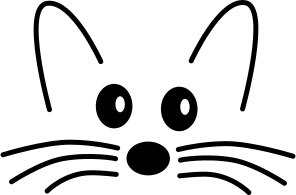
\includegraphics[width=1.4em]{squeak-logo}}}
\newcommand{\dothis}[1]{%
	\medskip
	\noindent\dothisicon
	\ifx#1\empty\else\quad\emph{#1}\fi
	\par\smallskip\nopagebreak}
% NB: To use this in an individual chapter, you must set:
%\graphicspath{{figures/} {../figures/}}
% at the head of the chapter.  Don't forget the final /
%=============================================================
%:Reader hints (hint)
%
% Indicates a non-obvious consequence 
\newcommand{\hint}[1]{\vspace{1ex}\noindent\fbox{\textsc{Astuce}} \emph{#1}}
%=================================================================
% graphics for Morphic handles
\newcommand{\grabHandle}{\raisebox{-0.2ex}{
\includegraphics[width=1em]{blackHandle}}}
\newcommand{\moveHandle}{\raisebox{-0.2ex}{
\includegraphics[width=1em]{moveHandle}}}
\newcommand{\debugHandle}{\raisebox{-0.2ex}{
\includegraphics[width=1em]{debugHandle}}}
% squeak-fr (added for Morphic handles)
\newcommand{\rotateHandle}{\raisebox{-0.2ex}{
\includegraphics[width=1em]{rotateHandle}}}
\newcommand{\viewerHandle}{\raisebox{-0.2ex}{
\includegraphics[width=1em]{viewerHandle}}}
% squeak-fr (add cloverHandle to use \clover in QuickTour.tex as alias
% todo 

%=============================================================
%:Highlighting Important stuff (doublebox)
%
% From Seaside book ...
\newsavebox{\SavedText}
\newlength{\InnerBoxRule}\setlength{\InnerBoxRule}{.75\fboxrule}
\newlength{\OuterBoxRule}\setlength{\OuterBoxRule}{1.5\fboxrule}
\newlength{\BoxSeparation}\setlength{\BoxSeparation}{1.5\fboxrule}
\addtolength{\BoxSeparation}{.5pt}
\newlength{\SaveBoxSep}\setlength{\SaveBoxSep}{2\fboxsep}
%
\newenvironment{doublebox}{\begin{lrbox}{\SavedText}
    \begin{minipage}{.75\textwidth}}
    {\end{minipage}\end{lrbox}\begin{center}
    \setlength{\fboxsep}{\BoxSeparation}\setlength{\fboxrule}{\OuterBoxRule}
    \fbox{\setlength{\fboxsep}{\SaveBoxSep}\setlength{\fboxrule}{\InnerBoxRule}%
      \fbox{\usebox{\SavedText}}}
  \end{center}}
% Use this:
%\newcommand{\important}[1]{\begin{doublebox}#1\end{doublebox}}


\newcommand{\important}[1]{
\noindent\rule{\textwidth}{2pt}\par
\textbf{Important!} #1 \par
\noindent\rule{\textwidth}{2pt}}

\newcommand{\note}[1]{
\noindent\rule{\textwidth}{2pt}\par
\noindent\textbf{Note} #1\par
\noindent\rule{\textwidth}{2pt}}

%=============================================================
%:Section depth
\setcounter{secnumdepth}{2}
%% for this to happen start the file with
%\ifx\wholebook\relax\else
%% $Author$ Martial
% $Date$ Wed Oct 10 13:34:55 CEST 2007
% $Revision$ source: SBE 12715 
% Last Changed Date: 2007-10-08 21:32:45 +0200 (Mon, 08 Oct 2007)
%=============================================================
% NB: documentclass must be set in main document.
% Allows book to be generated in multiple formats.
%=============================================================
%:Packages
%\usepackage[french]{babel}
\usepackage[T1]{fontenc}  %%%%%% really important to get the code directly in the text!
\usepackage{lmodern}
%\usepackage[scaled=0.85]{bookmanx} % needs another scale factor if used with \renewcommand{\sfdefault}{cmbr}
\usepackage{palatino}
%\usepackage[sc]{mathpazo}
%\linespread{1.05}
\usepackage[scaled=0.85]{helvet}
\usepackage{microtype}
\usepackage{graphicx}
\usepackage{theorem}
\usepackage[utf8]{inputenc}
% ON: pdfsync breaks the use of p{width} for tabular columns!
\ifdefined\usepdfsync\usepackage{pdfsync}\fi % Requires texlive 2007
%=============================================================
%:More packages
%Stef should check which ones are used!
%\usepackage{picinpar}
%\usepackage{layout}
%\usepackage{color}
%\definecolor{stefgris}{rgb}{0.85,0.85,0.85}
%\usepackage{enum}
%\usepackage{a4wide}
% \usepackage{fancyhdr}
\usepackage{ifthen}
\usepackage{float}
\usepackage{longtable}
\usepackage{makeidx}
\usepackage[nottoc]{tocbibind}
\usepackage{multicol}
\usepackage{booktabs}	% book-style tables
\usepackage{topcapt}	% enables \topcaption
\usepackage{multirow}
\usepackage{tabularx}
%\usepackage[bottom]{footmisc}
\usepackage{xspace}
\usepackage{alltt}
\usepackage{amssymb,textcomp}
\usepackage[usenames,dvipsnames]{color}
\usepackage{colortbl}
\usepackage[hang]{subfigure}\makeatletter\def\p@subfigure{\thefigure\,}\makeatother
\usepackage{rotating}
\usepackage{enumitem}	% apb: allows more control over tags in enumerations
\usepackage{verbatim}     % for comment environment
\usepackage{varioref}	% for page references that work
\labelformat{footnote}{\thechapter--#1} % to distinguish citations from jurabib
\usepackage{needspace}
\usepackage{isodateo} % enable \isodate
\usepackage[newparttoc]{titlesec}
\usepackage{titletoc}
\usepackage{eurosym}
\usepackage{wrapfig}

\usepackage[
	super,
	citefull=first,
	authorformat={allreversed,and},
	titleformat={commasep,italic}
]{jurabib} % citations as footnotes
\usepackage[
	colorlinks=true,
	linkcolor=black,
	urlcolor=black,
	citecolor=black
]{hyperref}   % should come last

%=============================================================
%:URL style
\makeatletter

\def\url@leostyle{%
  \@ifundefined{selectfont}{\def\UrlFont{\sf}}{\def\UrlFont{\sffamily}}}
% ajouter par Martial pour \traduit (met une dague dans les \doublebox
\def\thempfootnote{\fnsymbol{mpfootnote}}

\makeatother
% Now actually use the newly defined style.
\urlstyle{leo}
%=============================================================
%:Booleans
\newboolean{lulu}
\setboolean{lulu}{false}
\newcommand{\ifluluelse}[2]{\ifthenelse{\boolean{lulu}}{#1}{#2}}
%=============================================================
%:Names
\newcommand{\SUnit}{SUnit\xspace}
\newcommand{\sunit}{SUnit\xspace}
\newcommand{\xUnit}{$x$Unit\xspace}
\newcommand{\JUnit}{JUnit\xspace}
%\newcommand{\XP}{eXtreme Programming\xspace}
\newcommand{\st}{Smalltalk\xspace}
\newcommand{\Squeak}{Squeak\xspace}
\newcommand{\sq}{Squeak\xspace}
\newcommand{\sqmap}{SqueakMap\xspace}
\newcommand{\squeak}{Squeak\xspace}
%\newcommand{\sbe}{\url{scg.unibe.ch/SBE}\xspace}
%\newcommand{\sbe}{\url{squeakbyexample.org}\xspace}
\newcommand{\sbe}{\url{SqueakByExample.org}\xspace}
% squeak-fr: adresse de la version francaise
\newcommand{\spe}{\url{SqueakByExample.org/fr}\xspace}
\newcommand{\sba}{\url{SquareBracketAssociates.org}\xspace}

% squeak-fr: ajout de la \squeakdev pour eviter les problemes de
% changements d'url rencontres dans la VO:
\newcommand{\squeakdev}{\url{www.squeaksource.com/ImageForDevelopers}\xspace} %ou
%\newcommand{\squeakdev}{\url{squeak.ofset.org/squeak-dev}\xspace}

%=============================================================
%:Editorial comment macros
\newcommand{\nnbb}[2]{
    \fbox{\bfseries\sffamily\scriptsize#1}
    {\sf\small$\blacktriangleright$\textit{#2}$\blacktriangleleft$}
   }
\newcommand{\ab}[1]{\nnbb{Andrew}{#1}}
\newcommand{\sd}[1]{\nnbb{St\'{e}f}{#1}}
\newcommand{\md}[1]{\nnbb{Marcus}{#1}}
\newcommand{\on}[1]{\nnbb{Oscar}{#1}}
\newcommand{\damien}[1]{\nnbb{Damien}{#1}}
\newcommand{\lr}[1]{\nnbb{Lukas}{#1}}
\newcommand{\orla}[1]{\nnbb{Orla}{#1}}
%\newcommand{\here}{\nnbb{CONTINUE}{HERE}}
\newcommand{\here}{\nnbb{CONTINUE}{ICI}}

%=============================================================
%:Abbreviation macros
\newcommand{\ie}{\emph{c-\`a-d.}\xspace}
\newcommand{\cad}{\emph{c-\`a-d.}\xspace}
%\newcommand{\eg}{\emph{e.g.},\xspace}
\newcommand{\eg}{\emph{par ex.},\xspace}
\newcommand{\parex}{\emph{par ex.},\xspace}
\newcommand{\etc}{etc\xspace}
%=============================================================
%:Cross reference macros

% [squeak-fr] martial: remarquez les articles devant les noms
\newcommand{\charef}[1]{le chapitre~\ref{cha:#1}\xspace}
% note de martial: utilise dans chapitre Syntax.tex: a redefinir
\newcommand{\charefs}[2]{les chapitres~\ref{cha:#1} et \ref{cha:#2}\xspace}
\newcommand{\secref}[1]{la section~\ref{sec:#1}\xspace}
\newcommand{\figref}[1]{la figure~\ref{fig:#1}\xspace}
\newcommand{\Figref}[1]{La figure~\ref{fig:#1}\xspace}
\newcommand{\appref}[1]{l'annexe~\ref{app:#1}\xspace}
\newcommand{\tabref}[1]{la table~\ref{tab:#1}\xspace}
% defini pour le chapitre Messages.tex
\newcommand{\Tabref}[1]{La table~\ref{tab:#1}\xspace}

% APB: I removed trailing \xspace commands from these macros because
% \xspace mostly doesn't work.  If you want a space after your
% references, type one!
% ON: xspace has always worked just fine for me!  Please leave them in.
%
\newcommand{\ruleref}[1]{\ref{rule:#1}\xspace}
%
\newcommand{\egref}[1]{exemple~\ref{eg:#1}\xspace}
\newcommand{\Egref}[1]{Exemple~\ref{eg:#1}\xspace}
%
\newcommand{\scrref}[1]{script~\ref{scr:#1}\xspace}
\newcommand{\Scrref}[1]{Script~\ref{scr:#1}\xspace}
% t = the
\newcommand{\tscrref}[1]{le script~\ref{scr:#1}\xspace}
\newcommand{\Tscrref}[1]{Le script~\ref{scr:#1}\xspace}
%
\newcommand{\mthref}[1]{m\'ethode~\ref{mth:#1}\xspace}
\newcommand{\mthsref}[1]{m\'ethodes~\ref{mth:#1}\xspace}
\newcommand{\Mthref}[1]{M\'ethode~\ref{mth:#1}\xspace}
\newcommand{\tmthref}[1]{la m\'ethode~\ref{mth:#1}\xspace}
\newcommand{\Tmthref}[1]{La m\'ethode~\ref{mth:#1}\xspace}
%
\newcommand{\clsref}[1]{classe~\ref{cls:#1}\xspace}
\newcommand{\tclsref}[1]{la classe~\ref{cls:#1}\xspace}
\newcommand{\Tclsref}[1]{La classe~\ref{cls:#1}\xspace}
%=============================================================
%:Menu item macro
% for menu items, so we can change our minds on how to print them! (apb)
\definecolor{lightgray}{gray}{0.89}
\newcommand{\menu}[1]{{%
	\setlength{\fboxsep}{0pt}%
	\colorbox{lightgray}{{{\upshape\sffamily\strut \,#1\,}}}}}
% \newcommand{\menu}[1]{{%
% 	\fontfamily{lmr}\selectfont
% 	\upshape\textlangle{\sffamily #1}\textrangle}}
% For submenu items:
\newcommand{\go}{\,$\triangleright$\,}
% \newcommand{\go}{\,$\blacktriangleright$\,}
% For keyboard shortcuts:
%\newcommand{\short}[1]{\mbox{$\langle${\sc CMD}$\rangle$-#1}\xspace}
\newcommand{\short}[1]{\mbox{{\sc cmd}\hspace{0.08em}--\hspace{0.09em}#1}\xspace}
% For buttons:
\newcommand{\button}[1]{{%
	\setlength{\fboxsep}{0pt}%
	\fbox{{\upshape\sffamily\strut \,#1\,}}}}
\newcommand{\toolsflap}{l'onglet \textit{Tools}\xspace}
%=============================================================
%:Reader cues (do this)
%
% Indicate something the reader should try out.
\newcommand{\dothisicon}{\raisebox{-.5ex}{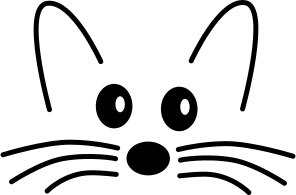
\includegraphics[width=1.4em]{squeak-logo}}}
\newcommand{\dothis}[1]{%
	\medskip
	\noindent\dothisicon
	\ifx#1\empty\else\quad\emph{#1}\fi
	\par\smallskip\nopagebreak}
% NB: To use this in an individual chapter, you must set:
%\graphicspath{{figures/} {../figures/}}
% at the head of the chapter.  Don't forget the final /
%=============================================================
%:Reader hints (hint)
%
% Indicates a non-obvious consequence 
\newcommand{\hint}[1]{\vspace{1ex}\noindent\fbox{\textsc{Astuce}} \emph{#1}}
%=================================================================
% graphics for Morphic handles
\newcommand{\grabHandle}{\raisebox{-0.2ex}{
\includegraphics[width=1em]{blackHandle}}}
\newcommand{\moveHandle}{\raisebox{-0.2ex}{
\includegraphics[width=1em]{moveHandle}}}
\newcommand{\debugHandle}{\raisebox{-0.2ex}{
\includegraphics[width=1em]{debugHandle}}}
% squeak-fr (added for Morphic handles)
\newcommand{\rotateHandle}{\raisebox{-0.2ex}{
\includegraphics[width=1em]{rotateHandle}}}
\newcommand{\viewerHandle}{\raisebox{-0.2ex}{
\includegraphics[width=1em]{viewerHandle}}}
% squeak-fr (add cloverHandle to use \clover in QuickTour.tex as alias
% todo 

%=============================================================
%:Highlighting Important stuff (doublebox)
%
% From Seaside book ...
\newsavebox{\SavedText}
\newlength{\InnerBoxRule}\setlength{\InnerBoxRule}{.75\fboxrule}
\newlength{\OuterBoxRule}\setlength{\OuterBoxRule}{1.5\fboxrule}
\newlength{\BoxSeparation}\setlength{\BoxSeparation}{1.5\fboxrule}
\addtolength{\BoxSeparation}{.5pt}
\newlength{\SaveBoxSep}\setlength{\SaveBoxSep}{2\fboxsep}
%
\newenvironment{doublebox}{\begin{lrbox}{\SavedText}
    \begin{minipage}{.75\textwidth}}
    {\end{minipage}\end{lrbox}\begin{center}
    \setlength{\fboxsep}{\BoxSeparation}\setlength{\fboxrule}{\OuterBoxRule}
    \fbox{\setlength{\fboxsep}{\SaveBoxSep}\setlength{\fboxrule}{\InnerBoxRule}%
      \fbox{\usebox{\SavedText}}}
  \end{center}}
% Use this:
%\newcommand{\important}[1]{\begin{doublebox}#1\end{doublebox}}


\newcommand{\important}[1]{
\noindent\rule{\textwidth}{2pt}\par
\textbf{Important!} #1 \par
\noindent\rule{\textwidth}{2pt}}

\newcommand{\note}[1]{
\noindent\rule{\textwidth}{2pt}\par
\noindent\textbf{Note} #1\par
\noindent\rule{\textwidth}{2pt}}

%=============================================================
%:Section depth
\setcounter{secnumdepth}{2}
%% for this to happen start the file with
%\ifx\wholebook\relax\else
%% $Author$ Martial
% $Date$ Wed Oct 10 13:34:55 CEST 2007
% $Revision$ source: SBE 12715 
% Last Changed Date: 2007-10-08 21:32:45 +0200 (Mon, 08 Oct 2007)
%=============================================================
% NB: documentclass must be set in main document.
% Allows book to be generated in multiple formats.
%=============================================================
%:Packages
%\usepackage[french]{babel}
\usepackage[T1]{fontenc}  %%%%%% really important to get the code directly in the text!
\usepackage{lmodern}
%\usepackage[scaled=0.85]{bookmanx} % needs another scale factor if used with \renewcommand{\sfdefault}{cmbr}
\usepackage{palatino}
%\usepackage[sc]{mathpazo}
%\linespread{1.05}
\usepackage[scaled=0.85]{helvet}
\usepackage{microtype}
\usepackage{graphicx}
\usepackage{theorem}
\usepackage[utf8]{inputenc}
% ON: pdfsync breaks the use of p{width} for tabular columns!
\ifdefined\usepdfsync\usepackage{pdfsync}\fi % Requires texlive 2007
%=============================================================
%:More packages
%Stef should check which ones are used!
%\usepackage{picinpar}
%\usepackage{layout}
%\usepackage{color}
%\definecolor{stefgris}{rgb}{0.85,0.85,0.85}
%\usepackage{enum}
%\usepackage{a4wide}
% \usepackage{fancyhdr}
\usepackage{ifthen}
\usepackage{float}
\usepackage{longtable}
\usepackage{makeidx}
\usepackage[nottoc]{tocbibind}
\usepackage{multicol}
\usepackage{booktabs}	% book-style tables
\usepackage{topcapt}	% enables \topcaption
\usepackage{multirow}
\usepackage{tabularx}
%\usepackage[bottom]{footmisc}
\usepackage{xspace}
\usepackage{alltt}
\usepackage{amssymb,textcomp}
\usepackage[usenames,dvipsnames]{color}
\usepackage{colortbl}
\usepackage[hang]{subfigure}\makeatletter\def\p@subfigure{\thefigure\,}\makeatother
\usepackage{rotating}
\usepackage{enumitem}	% apb: allows more control over tags in enumerations
\usepackage{verbatim}     % for comment environment
\usepackage{varioref}	% for page references that work
\labelformat{footnote}{\thechapter--#1} % to distinguish citations from jurabib
\usepackage{needspace}
\usepackage{isodateo} % enable \isodate
\usepackage[newparttoc]{titlesec}
\usepackage{titletoc}
\usepackage{eurosym}
\usepackage{wrapfig}

\usepackage[
	super,
	citefull=first,
	authorformat={allreversed,and},
	titleformat={commasep,italic}
]{jurabib} % citations as footnotes
\usepackage[
	colorlinks=true,
	linkcolor=black,
	urlcolor=black,
	citecolor=black
]{hyperref}   % should come last

%=============================================================
%:URL style
\makeatletter

\def\url@leostyle{%
  \@ifundefined{selectfont}{\def\UrlFont{\sf}}{\def\UrlFont{\sffamily}}}
% ajouter par Martial pour \traduit (met une dague dans les \doublebox
\def\thempfootnote{\fnsymbol{mpfootnote}}

\makeatother
% Now actually use the newly defined style.
\urlstyle{leo}
%=============================================================
%:Booleans
\newboolean{lulu}
\setboolean{lulu}{false}
\newcommand{\ifluluelse}[2]{\ifthenelse{\boolean{lulu}}{#1}{#2}}
%=============================================================
%:Names
\newcommand{\SUnit}{SUnit\xspace}
\newcommand{\sunit}{SUnit\xspace}
\newcommand{\xUnit}{$x$Unit\xspace}
\newcommand{\JUnit}{JUnit\xspace}
%\newcommand{\XP}{eXtreme Programming\xspace}
\newcommand{\st}{Smalltalk\xspace}
\newcommand{\Squeak}{Squeak\xspace}
\newcommand{\sq}{Squeak\xspace}
\newcommand{\sqmap}{SqueakMap\xspace}
\newcommand{\squeak}{Squeak\xspace}
%\newcommand{\sbe}{\url{scg.unibe.ch/SBE}\xspace}
%\newcommand{\sbe}{\url{squeakbyexample.org}\xspace}
\newcommand{\sbe}{\url{SqueakByExample.org}\xspace}
% squeak-fr: adresse de la version francaise
\newcommand{\spe}{\url{SqueakByExample.org/fr}\xspace}
\newcommand{\sba}{\url{SquareBracketAssociates.org}\xspace}

% squeak-fr: ajout de la \squeakdev pour eviter les problemes de
% changements d'url rencontres dans la VO:
\newcommand{\squeakdev}{\url{www.squeaksource.com/ImageForDevelopers}\xspace} %ou
%\newcommand{\squeakdev}{\url{squeak.ofset.org/squeak-dev}\xspace}

%=============================================================
%:Editorial comment macros
\newcommand{\nnbb}[2]{
    \fbox{\bfseries\sffamily\scriptsize#1}
    {\sf\small$\blacktriangleright$\textit{#2}$\blacktriangleleft$}
   }
\newcommand{\ab}[1]{\nnbb{Andrew}{#1}}
\newcommand{\sd}[1]{\nnbb{St\'{e}f}{#1}}
\newcommand{\md}[1]{\nnbb{Marcus}{#1}}
\newcommand{\on}[1]{\nnbb{Oscar}{#1}}
\newcommand{\damien}[1]{\nnbb{Damien}{#1}}
\newcommand{\lr}[1]{\nnbb{Lukas}{#1}}
\newcommand{\orla}[1]{\nnbb{Orla}{#1}}
%\newcommand{\here}{\nnbb{CONTINUE}{HERE}}
\newcommand{\here}{\nnbb{CONTINUE}{ICI}}

%=============================================================
%:Abbreviation macros
\newcommand{\ie}{\emph{c-\`a-d.}\xspace}
\newcommand{\cad}{\emph{c-\`a-d.}\xspace}
%\newcommand{\eg}{\emph{e.g.},\xspace}
\newcommand{\eg}{\emph{par ex.},\xspace}
\newcommand{\parex}{\emph{par ex.},\xspace}
\newcommand{\etc}{etc\xspace}
%=============================================================
%:Cross reference macros

% [squeak-fr] martial: remarquez les articles devant les noms
\newcommand{\charef}[1]{le chapitre~\ref{cha:#1}\xspace}
% note de martial: utilise dans chapitre Syntax.tex: a redefinir
\newcommand{\charefs}[2]{les chapitres~\ref{cha:#1} et \ref{cha:#2}\xspace}
\newcommand{\secref}[1]{la section~\ref{sec:#1}\xspace}
\newcommand{\figref}[1]{la figure~\ref{fig:#1}\xspace}
\newcommand{\Figref}[1]{La figure~\ref{fig:#1}\xspace}
\newcommand{\appref}[1]{l'annexe~\ref{app:#1}\xspace}
\newcommand{\tabref}[1]{la table~\ref{tab:#1}\xspace}
% defini pour le chapitre Messages.tex
\newcommand{\Tabref}[1]{La table~\ref{tab:#1}\xspace}

% APB: I removed trailing \xspace commands from these macros because
% \xspace mostly doesn't work.  If you want a space after your
% references, type one!
% ON: xspace has always worked just fine for me!  Please leave them in.
%
\newcommand{\ruleref}[1]{\ref{rule:#1}\xspace}
%
\newcommand{\egref}[1]{exemple~\ref{eg:#1}\xspace}
\newcommand{\Egref}[1]{Exemple~\ref{eg:#1}\xspace}
%
\newcommand{\scrref}[1]{script~\ref{scr:#1}\xspace}
\newcommand{\Scrref}[1]{Script~\ref{scr:#1}\xspace}
% t = the
\newcommand{\tscrref}[1]{le script~\ref{scr:#1}\xspace}
\newcommand{\Tscrref}[1]{Le script~\ref{scr:#1}\xspace}
%
\newcommand{\mthref}[1]{m\'ethode~\ref{mth:#1}\xspace}
\newcommand{\mthsref}[1]{m\'ethodes~\ref{mth:#1}\xspace}
\newcommand{\Mthref}[1]{M\'ethode~\ref{mth:#1}\xspace}
\newcommand{\tmthref}[1]{la m\'ethode~\ref{mth:#1}\xspace}
\newcommand{\Tmthref}[1]{La m\'ethode~\ref{mth:#1}\xspace}
%
\newcommand{\clsref}[1]{classe~\ref{cls:#1}\xspace}
\newcommand{\tclsref}[1]{la classe~\ref{cls:#1}\xspace}
\newcommand{\Tclsref}[1]{La classe~\ref{cls:#1}\xspace}
%=============================================================
%:Menu item macro
% for menu items, so we can change our minds on how to print them! (apb)
\definecolor{lightgray}{gray}{0.89}
\newcommand{\menu}[1]{{%
	\setlength{\fboxsep}{0pt}%
	\colorbox{lightgray}{{{\upshape\sffamily\strut \,#1\,}}}}}
% \newcommand{\menu}[1]{{%
% 	\fontfamily{lmr}\selectfont
% 	\upshape\textlangle{\sffamily #1}\textrangle}}
% For submenu items:
\newcommand{\go}{\,$\triangleright$\,}
% \newcommand{\go}{\,$\blacktriangleright$\,}
% For keyboard shortcuts:
%\newcommand{\short}[1]{\mbox{$\langle${\sc CMD}$\rangle$-#1}\xspace}
\newcommand{\short}[1]{\mbox{{\sc cmd}\hspace{0.08em}--\hspace{0.09em}#1}\xspace}
% For buttons:
\newcommand{\button}[1]{{%
	\setlength{\fboxsep}{0pt}%
	\fbox{{\upshape\sffamily\strut \,#1\,}}}}
\newcommand{\toolsflap}{l'onglet \textit{Tools}\xspace}
%=============================================================
%:Reader cues (do this)
%
% Indicate something the reader should try out.
\newcommand{\dothisicon}{\raisebox{-.5ex}{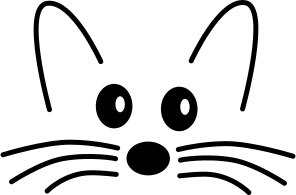
\includegraphics[width=1.4em]{squeak-logo}}}
\newcommand{\dothis}[1]{%
	\medskip
	\noindent\dothisicon
	\ifx#1\empty\else\quad\emph{#1}\fi
	\par\smallskip\nopagebreak}
% NB: To use this in an individual chapter, you must set:
%\graphicspath{{figures/} {../figures/}}
% at the head of the chapter.  Don't forget the final /
%=============================================================
%:Reader hints (hint)
%
% Indicates a non-obvious consequence 
\newcommand{\hint}[1]{\vspace{1ex}\noindent\fbox{\textsc{Astuce}} \emph{#1}}
%=================================================================
% graphics for Morphic handles
\newcommand{\grabHandle}{\raisebox{-0.2ex}{
\includegraphics[width=1em]{blackHandle}}}
\newcommand{\moveHandle}{\raisebox{-0.2ex}{\includegraphics[width=1em]{moveHandle}}}
\newcommand{\debugHandle}{\raisebox{-0.2ex}{\includegraphics[width=1em]{debugHandle}}}
% squeak-fr (added for Morphic handles)
\newcommand{\rotateHandle}{\raisebox{-0.2ex}{\includegraphics[width=1em]{rotateHandle}}}
\newcommand{\viewerHandle}{\raisebox{-0.2ex}{\includegraphics[width=1em]{viewerHandle}}}
% squeak-fr (add cloverHandle to use \clover in QuickTour.tex as alias
% todo 

%=============================================================
%:Highlighting Important stuff (doublebox)
%
% From Seaside book ...
\newsavebox{\SavedText}
\newlength{\InnerBoxRule}\setlength{\InnerBoxRule}{.75\fboxrule}
\newlength{\OuterBoxRule}\setlength{\OuterBoxRule}{1.5\fboxrule}
\newlength{\BoxSeparation}\setlength{\BoxSeparation}{1.5\fboxrule}
\addtolength{\BoxSeparation}{.5pt}
\newlength{\SaveBoxSep}\setlength{\SaveBoxSep}{2\fboxsep}
%
\newenvironment{doublebox}{\begin{lrbox}{\SavedText}
    \begin{minipage}{.75\textwidth}}
    {\end{minipage}\end{lrbox}\begin{center}
    \setlength{\fboxsep}{\BoxSeparation}\setlength{\fboxrule}{\OuterBoxRule}
    \fbox{\setlength{\fboxsep}{\SaveBoxSep}\setlength{\fboxrule}{\InnerBoxRule}%
      \fbox{\usebox{\SavedText}}}
  \end{center}}
% Use this:
%\newcommand{\important}[1]{\begin{doublebox}#1\end{doublebox}}


\newcommand{\important}[1]{
\noindent\rule{\textwidth}{2pt}\par
\textbf{Important!} #1 \par
\noindent\rule{\textwidth}{2pt}}

\newcommand{\note}[1]{
\noindent\rule{\textwidth}{2pt}\par
\noindent\textbf{Note} #1\par
\noindent\rule{\textwidth}{2pt}}

%=============================================================
%:Section depth
\setcounter{secnumdepth}{2}
%% for this to happen start the file with
%\ifx\wholebook\relax\else
%\input{../common.tex}
%\begin{document}
%\fi
% and terminate by
% \ifx\wholebook\relax\else\end{document}\fi

\DeclareGraphicsExtensions{.pdf, .jpg, .png}
%=============================================================
%:PDF setup
\hypersetup{
%   a4paper,
%   pdfstartview=FitV,
%   colorlinks,
%   linkcolor=darkblue,
%   citecolor=darkblue,
%   pdftitle={Squeak by Example},
pdftitle={Squeak par l'exemple},
   pdfauthor={Andrew Black, St\'ephane Ducasse,	Oscar Nierstrasz,
Damien Pollet},
   pdfkeywords={Smalltalk, Squeak, Programmation Orient\'ee Objet},
pdfsubject={Informatique, Computer Science}
}
%=============================================================
%:Page layout and appearance
%
% \renewcommand{\headrulewidth}{0pt}
\renewcommand{\chaptermark}[1]{\markboth{#1}{}}
\renewcommand{\sectionmark}[1]{\markright{\thesection\ #1}}
\renewpagestyle{plain}[\small\itshape]{%
	\setheadrule{0pt}%
	\sethead[][][]{}{}{}%
	\setfoot[][][]{}{}{}}
\renewpagestyle{headings}[\small\itshape]{%
	\setheadrule{0pt}%
	\setmarks{chapter}{section}%
	\sethead[\thepage][][\chaptertitle]{\sectiontitle}{}{\thepage}%
	\setfoot[][][]{}{}{}}
% pagestyle for tableofcontents + index (martial: 2008/04/23)
\newpagestyle{newheadings}[\small\itshape]{%
	\setheadrule{0pt}%
	\setmarks{chapter}{section}%
	\sethead[\thepage][][\chaptertitle]{\chaptertitle}{}{\thepage}%
	\setfoot[][][]{}{}{}}
%=============================================================
%:Title section setup and TOC numbering depth
\setcounter{secnumdepth}{1}
\setcounter{tocdepth}{1}
\titleformat{\part}[display]{\centering}{\huge\partname\ \thepart}{1em}{\Huge\textbf}[]
\titleformat{\chapter}[display]{}{\huge\chaptertitlename\ \thechapter}{1em}{\Huge\raggedright\textbf}[]
\titlecontents{part}[3pc]{%
		\pagebreak[2]\addvspace{1em plus.4em minus.2em}%
		\leavevmode\large\bfseries}
	{\contentslabel{3pc}}{\hspace*{-3pc}}
	{}[\nopagebreak]
\titlecontents{chapter}[3pc]{%
		\pagebreak[0]\addvspace{1em plus.2em minus.2em}%
		\leavevmode\bfseries}
	{\contentslabel{3pc}}{}
	{\hfill\contentspage}[\nopagebreak]
\dottedcontents{section}[3pc]{}{3pc}{1pc}
\dottedcontents{subsection}[3pc]{}{0pc}{1pc}
% \dottedcontents{subsection}[4.5em]{}{0pt}{1pc}
% Make \cleardoublepage insert really blank pages http://www.tex.ac.uk/cgi-bin/texfaq2html?label=reallyblank
\let\origdoublepage\cleardoublepage
\newcommand{\clearemptydoublepage}{%
  \clearpage
  {\pagestyle{empty}\origdoublepage}}
\let\cleardoublepage\clearemptydoublepage % see http://www.tex.ac.uk/cgi-bin/texfaq2html?label=patch
%=============================================================
%:FAQ macros (for FAQ chapter)
\newtheorem{faq}{FAQ}
\newcommand{\answer}{\paragraph{R\'eponse}\ }
%=============================================================
%:Listings package configuration
\usepackage{listings}
\newcommand{\caret}{\makebox{\raisebox{0.4ex}{\footnotesize{$\wedge$}}}}
\lstdefinelanguage{Smalltalk}{
%  morekeywords={self,super,true,false,nil,thisContext}, % This is overkill
  morestring=[d]',
  morecomment=[s]{"}{"},
  alsoletter={\#:},
  escapechar={!},
  escapebegin=\itshape, % comment-like by default (Martial 11/2007)
  literate=
    {BANG}{!}1
    {UNDERSCORE}{\_}1
    {\\st}{Smalltalk}9 % convenience -- in case \st occurs in code
    % {'}{{\textquotesingle}}1 % replaced by upquote=true in \lstset
    {_}{{$\leftarrow$}}1
    {>>>}{{\sep}}1
    {^}{{$\uparrow$}}1
    {~}{{$\sim$}}1
    {-}{{\sf -\hspace{-0.13em}-}}1  % the goal is to make - the same width as +
    {+}{\raisebox{0.08ex}{+}}1		% and to raise + off the baseline to match -
    {-->}{{\quad$\longrightarrow$\quad}}3
	, % Don't forget the comma at the end!
  tabsize=4
}[keywords,comments,strings]
% ajout pour les échappements dans les codes
% indispensable pour mettre le code en emphase (cf. Model.tex) 
\newcommand{\codeify}[1]{\NoAutoSpaceBeforeFDP#1\AutoSpaceBeforeFDP}
\newcommand{\normcomment}[1]{\emph{#1}} %cf. Streams
\newcommand{\normcode}[1]{\emph{\codeify{#1}}} %cf. Streams
\newcommand{\emcode}[1]{\textbf{\normcode{#1}}} % Martial 11/2007
\lstset{language=Smalltalk,
	basicstyle=\sffamily,
	keywordstyle=\color{black}\bfseries,
	% stringstyle=\ttfamily, % Ugly! do we really want this? -- on
	%commentstyle=\itshape,
	mathescape=true,
	showstringspaces=false,
	keepspaces=true,
	breaklines=true,
	breakautoindent=true,
	lineskip={-1pt}, % Ugly hack
	upquote=true, % straight quote; requires textcomp package
	columns=fullflexible} % no fixed width fonts
% In-line code (literal)
% Normally use this for all in-line code:
\newcommand{\ct}{\lstinline[mathescape=false,basicstyle={\sffamily\upshape}]}
% apb 2007.8.28 added the \upshape declaration to avoid getting italicized code in \dothis{ } sections.
% In-line code (latex enabled)
% Use this only in special situations where \ct does not work
% (within section headings ...):

% [squeak-fr] Modification de \lct suivant les indications de Martial Boniou
\newcommand{\lct}[1]{\textsf{\textup{\NoAutoSpaceBeforeFDP #1
\AutoSpaceBeforeFDP}}} %\xspace

% Use these for system categories and protocols:
\newcommand{\scat}[1]{\emph{\textsf{#1}}\xspace}
\newcommand{\pkg}[1]{\emph{\textsf{#1}}\xspace}
\newcommand{\prot}[1]{\emph{\textsf{#1}}\xspace}
% Code environments
% NB: the arg is for tests
% Only code and example environments may be tests
\lstnewenvironment{code}[1]{%
	\lstset{%
		frame=lines,
		mathescape=false
	}
}{}
\def\ignoredollar#1{}
%=============================================================
%:Code environments (method, script ...)
% NB: the third arg is for tests
% Only code and example environments may be tests
\lstnewenvironment{example}[3][defaultlabel]{%
	\renewcommand{\lstlistingname}{Exemple}%
	\lstset{
		frame=lines,
		mathescape=false,
		caption={\emph{#2}},
		label={eg:#1}
	}
}{}
\lstnewenvironment{script}[2][defaultlabel]{%
\renewcommand{\lstlistingname}{Script}%
	\lstset{
		frame=lines,
		mathescape=false,
		name={Script},
		caption={\emph{#2}},
		label={scr:#1}
	}
}{}
%I could not find a way yo get the Experiment #numb followed by the caption in a black box
%\colorbox{black}{\makebox[\textwidth]{  \color{white} {\large {\bfseries Experiment 3-1 (crear i moure un robot)}} }}
\lstnewenvironment{experiment}[2][defaultlabel]{%
%\noindent\rule{\textwidth}{2pt}\vspace{-0.8cm}
\renewcommand{\lstlistingname}{Experiment}%
	\lstset{
		frame=none,
		rulecolor=\color{black},
		mathescape=false,
		name={Experiment},
		caption={\emph{#2}},
		label={scr:#1}
	}
}{%\vspace{-0.5cm}\noindent\rule{\textwidth}{2pt}
}

\lstnewenvironment{method}[2][defaultlabel]{%
	\renewcommand{\lstlistingname}{Method}%
	\lstset{
		frame=lines,
		mathescape=false,
		name={M\'ethode},
		caption={\emph{#2}},
		label={mth:#1}
	}
}{}
\lstnewenvironment{methods}[2][defaultlabel]{% just for multiple methods at once
	\renewcommand{\lstlistingname}{Methods}%
	\lstset{
		frame=lines,
		mathescape=false,
		name={M\'ethode},
		caption={\emph{#2}},
		label={mth:#1}
	}
}{}
\lstnewenvironment{numMethod}[2][defaultlabel]{%
	\renewcommand{\lstlistingname}{Method}%
	\lstset{
		numbers=left,
		numberstyle={\tiny\sffamily},
		frame=lines,
		mathescape=false,
		name={M\'ethode},
		caption={\emph{#2}},
		label={mth:#1}
	}
}{}
% \lstnewenvironment{classdef}[2][defaultlabel]{%
% 	\renewcommand{\lstlistingname}{Classe}%
% 	\lstset{
% 		frame=lines,
% 		mathescape=false,
% 		name={Classe},
% 		caption={\emph{#2}},
% 		label={cls:#1}
% 	}
% }{}

%%%%%%%%%%%%%%%%%%%%%%%%%%%%%%%%%%%%%%%%%%%%%%%%%%%%%%%%%%%%%%%%%%%%%%%%%%%%%%%%%%%%%%%%%%%%%%%%%
%%From the original book latex template
%%%%%%%%%%%%%%%%%%%%%%%%%%%%%%%%%%%%%%%%%%%%%%%%%%%%%%%%%%%%%%%%%%%%%%%%%%%%%%%%%%%%%%%%%%%%%%%%%
\theoremstyle{break}
{\theorembodyfont{\rmfamily}\theoremstyle{break}
\newtheorem{privScript}{Script}[chapter]
%\newtheorem{privMethod}{Method}[chapter]
\newtheorem{privExercise}{Experiment}[chapter]}

% \theoremstyle{break}
% {\theorembodyfont{\rmfamily} \newtheorem{privMethod}{Method}[chapter]}

%class
\theoremstyle{break}
{\theorembodyfont{\rmfamily} \newtheorem{privClassDef}{Class}[chapter]}

%important
\theoremstyle{break}
{\theorembodyfont{\rmfamily} \newtheorem{privTemplate}{Important Messages}[chapter]}

% experiment
\newenvironment{exercise}
    {\begin{privExercise}\mbox{}\\}
    {\end{privExercise}}


%%% for figure
\newsavebox{\ScriptFigure}
\newlength{\ScriptWidth}
\newlength{\FigureWidth}

%%%%%%%%%%%%%%%%%%%%%%%%%%%%%%%%%%%%%%%%%%%%%%%%%%%%%%%%%%%%%%%%%%%%%%%%%%%%%%%%
\newenvironment{scriptfig}[3][0.6]
   {\setlength{\ScriptWidth}{\linewidth*\real{#1}}%
   \setlength{\FigureWidth}{\linewidth-(\linewidth*\real{#1})}%
   \savebox{\ScriptFigure}%
	{\parbox{\FigureWidth}{\includegraphics[width=0.98\FigureWidth]{#2}}}%
   \par\noindent\begin{minipage}{\linewidth}\hrule\vskip 0.2cm\begin{minipage}[c]{\ScriptWidth}%
   \begin{stefscript}[{\em #3}]\begin{alltt}\sffamily}
   {\end{alltt}\end{stefscript}\end{minipage}\hfill
   \usebox{\ScriptFigure}
   \vskip 1ex\hrule\end{minipage}\vskip 1ex\par}

%%%%%%%%%%%%%%%%%%%%%%%%%%%%%%%%%%%%%%%%%%%%%%%%%%%%%%%%%%%%%%%%%%%%%%%%%%%%%%%%
%% to be able to specify the complete set of values for includegraphics
%% may be will be changed but not the interface
\newenvironment{scriptfigwithsize}[3][0.6]
   {\setlength{\ScriptWidth}{\linewidth*\real{#1}}%
   \setlength{\FigureWidth}{\linewidth-(\linewidth*\real{#1})}%
   \savebox{\ScriptFigure}{\parbox{\FigureWidth}{\raggedleft{#2}}}%
   \par\noindent\begin{minipage}{\linewidth}\hrule\vskip 0.3cm\begin{minipage}[c]{\ScriptWidth}%
   \begin{stefscript}[{\em #3}]\begin{alltt}\sffamily}
   {\end{alltt}\end{stefscript}\end{minipage}\hfill
   \usebox{\ScriptFigure}
   \vskip 1ex\hrule\end{minipage}\vskip 1ex\par}

% \newenvironment{methodfig}[2][0.6]
%    {\setlength{\ScriptWidth}{\linewidth*\real{#1}}%
%    \setlength{\FigureWidth}{\linewidth-(\linewidth*\real{#1})}%
%    \savebox{\ScriptFigure}{\parbox{\FigureWidth}{\includegraphics[width=.98\FigureWidth]{#2}}}%
%    \par\noindent\rule{\linewidth}{1mm}
%    \\[-0.3cm]\noindent\rule{\linewidth}{0.1mm}
%    \noindent\begin{minipage}[c]{\ScriptWidth}\begin{privMethod}\begin{alltt}\sffamily}
%    {\end{alltt}\end{privMethod}\end{minipage}\hfill
%    \usebox{\ScriptFigure} \vskip 1ex\hrule\vskip 1ex\par}

% \newenvironment{method}
% {\par\noindent\begin{minipage}{\linewidth}\vspace{0.2cm}\begin{privMethod}\begin{nminipage}\vspace{-0.2cm}\rule{\linewidth}{1mm}\\[-0.6cm]\rule{\linewidth}{0.1mm}\end{nminipage}\hspace*{\scriptindent}\codesize\begin{nalltt}\vspace{-0.2cm}}
% {\end{nalltt}\normalsize\vspace{-0.1cm}\hrule\end{privMethod}\vspace{0.2cm}\end{minipage}}


% \newenvironment{classdef}
% {\par\noindent\begin{minipage}{\linewidth}\vspace{0.2cm}\begin{privClassDef}\begin{nminipage}\vspace{-0.2cm}\rule{\linewidth}{1mm}\\[-0.6cm]\rule{\linewidth}{0.1mm}\end{nminipage}\hspace*{\scriptindent}\codesize\begin{nalltt}\vspace{-0.2cm}}
% {\end{nalltt}\normalsize\vspace{-0.1cm}\hrule\end{privClassDef}\vspace{0.2cm}\end{minipage}}


% \newenvironment{template}
% {\par\noindent\begin{minipage}{\linewidth}\vspace{0.3cm}\begin{privTemplate}\begin{nminipage}\vspace{-0.4cm}\rule{\linewidth}{0.1mm}\end{nminipage}\hspace*{\scriptindent}\begin{nalltt}\vspace{-0.7cm}}
% {\end{nalltt}\vspace{-0.1cm}\hrule\end{privTemplate}\end{minipage}\vspace{0.3cm}}

\newenvironment{exofig}[2][0.7]
   {\setlength{\ScriptWidth}{\linewidth*\real{#1}}
   \setlength{\FigureWidth}{\linewidth-(\linewidth*\real{#1})}
   \savebox{\ScriptFigure}{\parbox{\FigureWidth}{\raggedleft{\includegraphics[width=.98\FigureWidth]{#2}}}}
   \par\noindent\begin{minipage}{\linewidth}\hrule\vskip 0.3cm\begin{minipage}[c]{\ScriptWidth}%
   \begin{privExercise}}
   {\end{privExercise}\end{minipage}\hfill
   \usebox{\ScriptFigure}
   \vskip 1ex\hrule\end{minipage}\vskip 1ex\par}

\newenvironment{exofigwithsize}[2][0.7]
   {\setlength{\ScriptWidth}{\linewidth*\real{#1}}
   \setlength{\FigureWidth}{\linewidth-(\linewidth*\real{#1})}
   \savebox{\ScriptFigure}{\parbox{\FigureWidth}{\raggedleft{#2}}}
   \par\noindent\begin{minipage}{\linewidth}\hrule\vskip 0.3cm\begin{minipage}[c]{\ScriptWidth}%
   \begin{privExercise}}
   {\end{privExercise}\end{minipage}\hfill\usebox{\ScriptFigure}
   \vskip 1ex\hrule\end{minipage}\vskip 1ex\par}

\newenvironment{exofigwithsizeandtitle}[3][0.7]
   {\setlength{\ScriptWidth}{\linewidth*\real{#1}}
   \setlength{\FigureWidth}{\linewidth-(\linewidth*\real{#1})}
   \savebox{\ScriptFigure}{\parbox{\FigureWidth}{\raggedleft{#2}}}
   \vskip 0.3cm\par\noindent\begin{minipage}{\linewidth}\hrule\vskip 0.1cm\begin{minipage}[c]{\ScriptWidth}%
   \begin{privExercise}[\em{#3}]}
   {\end{privExercise}\end{minipage}\hfill\usebox{\ScriptFigure}
   \vskip 1ex\hrule\end{minipage}\vskip 1ex\par}

\newenvironment{exofigwithtitle}[3][0.7]
   {\setlength{\ScriptWidth}{\linewidth*\real{#1}}
   \setlength{\FigureWidth}{\linewidth-(\linewidth*\real{#1})}
   \savebox{\ScriptFigure}{\parbox{\FigureWidth}{\raggedleft{\includegraphics[width=.98\FigureWidth]{#2}}}}
   \par\noindent\begin{minipage}{\linewidth}\hrule\vskip 0.3cm\begin{minipage}[c]{\ScriptWidth}%
   \begin{privExercise}[\em{#3}]}
   {\end{privExercise}\end{minipage}\hfill
   \usebox{\ScriptFigure}
   \vskip 1ex\hrule\end{minipage}\vskip 1ex\par}


\newenvironment{exonofigwithtitle}[3][0.7]
   {\setlength{\ScriptWidth}{\linewidth*\real{#1}}
   \setlength{\FigureWidth}{\linewidth-(\linewidth*\real{#1})}
   \savebox{\ScriptFigure}{\parbox{\FigureWidth}{\raggedleft{\includegraphics[width=.98\FigureWidth]{#2}}}}
   \par\noindent\begin{minipage}{\linewidth}\hrule\vskip 0.3cm\begin{minipage}[c]{\ScriptWidth}%
   \begin{privExercise}[\em{#3}]}
   {\end{privExercise}\end{minipage}\hfill
   \usebox{\ScriptFigure}
   \vskip 1ex\hrule\end{minipage}\vskip 1ex\par}

\newenvironment{exonofig}
   {\par\noindent\begin{minipage}[t]{\linewidth}\noindent\begin{privExercise}}
   {\end{privExercise}\end{minipage}\vspace{0.5cm}\par}

\newenvironment{exonofigtitle}[1]
   {\par\noindent\begin{minipage}[t]{\linewidth}\noindent\begin{privExercise}[\em{#1}]}
   {\end{privExercise}\end{minipage}\vspace{0.5cm}\par}
		
% \newenvironment{solfig}[3][0.5]
%    {\setlength{\ScriptWidth}{\linewidth*\real{#1}}
%    \setlength{\FigureWidth}{\linewidth-\linewidth*\real{#1}}
%    \savebox{\ScriptFigure}{\parbox{\FigureWidth}{\includegraphics[width=.9\linewidth]{#2}}}
%    \par\noindent\vskip 1ex\hrule\vskip 1ex\begin{minipage}[t]{\ScriptWidth}
%    {\bf Solution #3} \begin{alltt}\sffamily}
%    {\end{alltt}\end{minipage}\hfill
%    \usebox{\ScriptFigure}
%    \vskip 1ex\hrule\vskip 1ex\par}
% 
% \newenvironment{solnofig}[1]
%    {\par\noindent\vskip 1ex\hrule\vskip 1ex\begin{minipage}[t]{\ScriptWidth}
%    {\bf Solution #1} \begin{alltt}\sffamily}
%    {\end{alltt}\end{minipage}\hfill
%    \vskip 1ex\hrule\vskip 1ex\par}
% 
% \newenvironment{exoscript}[3][0.5]
%    {\setlength{\ScriptWidth}{\linewidth*\real{#1}}
%     \setlength{\FigureWidth}{\linewidth-\linewidth*\real{#1}}
%     \savebox{\ScriptFigure}{\begin{minipage}\begin{alltt}\sffamily#3\end{alltt}\end{minipage}}
%     \par\noindent\vskip 1ex\hrule\vskip 1ex\begin{minipage}[t]{\ScriptWidth}
%     \begin{privExercise}}
%     {\end{privExercise}\end{minipage}\hfill
%     \usebox{\ScriptFigure}
% \vskip 1ex\hrule\vskip 1ex\par}


%%%%%%%%%%%%%%%%%%%%%%%%%%%%%%%%%%%%%%%%%%%%%%%%%%%%%%%%%%%%%%%%
%% Define the indentation from which the code script starts
%\newlength{\scriptindent}
%\setlength{\scriptindent}{.3cm}
%%%%%%%%%%%%%%%%%%%%%%%%%%%%%%%%%%%%%%%%%%%%%%%%%%%%%%%%%%%%%%%%
%% Method presentation 
%\newlength{\methodindent}
%\newlength{\methodwordlength}
%\newlength{\aftermethod}
%\setlength{\methodindent}{0.2cm}
%\settowidth{\methodwordlength}{\ M\'ethode\ }

%%%%%%%%%%%%%%%%%%%%%%%%%%%%%%%%%%%%%%%%%%%%%%%%%%%%%%%%%%%%%%%%
\theoremstyle{break}
{\theorembodyfont{\rmfamily} \newtheorem{fonction}{Script}[chapter]}

\newsavebox{\fminibox}
\newlength{\fminilength}
% Fait un truc encadre
\newenvironment{fminipage}[1][\linewidth]
  {\setlength{\fminilength}{#1-2\fboxsep-2\fboxrule}
        \begin{lrbox}{\fminibox}\begin{minipage}{\fminilength}}
  { \end{minipage}\end{lrbox}\noindent\fbox{\usebox{\fminibox}}}

% Pareil mais pas encadre (a utiliser pour ne pas couper une fonction en 2)
\newenvironment{nminipage}[1][\linewidth]
  {\setlength{\fminilength}{#1}
        \begin{lrbox}{\fminibox}\begin{minipage}{\fminilength}}
  { \end{minipage}\end{lrbox}\noindent\mbox{\usebox{\fminibox}}}

% Un alltt encadre
\newenvironment{falltt}
  {\vspace*{0.3cm}\begin{fminipage}\begin{alltt}\ttfamily}
  {\end{alltt}\end{fminipage}\vspace*{0.3cm}}

% Un alltt pas encadre
\newenvironment{nalltt}
  {\vspace*{0.3cm}\begin{nminipage}\begin{alltt}\sffamily}
  {\end{alltt}\end{nminipage}\vspace*{0.3cm}}

% Une fonction encadree
\newenvironment{ffonction}[1]
  {\begin{fonction}[#1]\begin{fminipage}\begin{alltt}\ttfamily\rule{\linewidth}{0.5pt}}
{\end{alltt}\end{fminipage}\end{fonction}}


\theoremstyle{break}
{\theorembodyfont{\rmfamily} \newtheorem{stefscript}{Script}[chapter]}

\theoremstyle{break}
{\theorembodyfont{\rmfamily} \newtheorem{exampleScript}{Examples}[chapter]}


%%Not used
\newenvironment{ncscript}[1]
{\vspace{-0.5cm}\begin{stefscript}[#1]\begin{nalltt}\rule{\linewidth}{1.5pt}\vspace{-0.1cm}
\hspace*{\scriptindent}\begin{nalltt}}
{\end{nalltt}\vspace{-0.5cm}\hrule\end{nalltt}\end{stefscript}\vspace{-0.5cm}}
%%Not used
\newenvironment{soluscript}[1]
{\begin{nalltt}\textbf{Solution du script : #1.}\\
\rule{\linewidth}{1.5pt}
\hspace*{\scriptindent}\begin{nalltt}}
{\end{nalltt}\vspace{-0.5cm}\hrule\end{nalltt}\vspace{-0.5cm}\\}




\newenvironment{scriptwithtitle}[1]
{\vspace{-0.3cm}\begin{stefscript}[{\em #1}]\begin{nalltt}\rule{\linewidth}{1.5pt}\vspace{-0.3cm}\hspace*{\scriptindent}\begin{nalltt}\codesize}
{\normalsize\end{nalltt}\vspace{-0.2cm}\hrule\end{nalltt}\end{stefscript}\vspace{-0.5cm}}

\newenvironment{scriptwithouttitle}
{\vspace{-0.5cm}\begin{stefscript}\codesize\begin{nalltt}\rule{\linewidth}{1.5pt}\vspace{-0.1cm}
\hspace*{\scriptindent}\begin{nalltt}}
{\end{nalltt}\vspace{-0.5cm}\hrule\end{nalltt}\normalsize\end{stefscript}\vspace{-0.5cm}}

% \newenvironment{example}
% {\vspace{-0.5cm}\begin{exampleScript}\codesize\begin{nalltt}\rule{\linewidth}{1.5pt}\vspace{-0.1cm}\hspace*{\scriptindent}\begin{nalltt}}
% {\end{nalltt}\vspace{-0.2cm}\hrule\end{nalltt}\normalsize\end{exampleScript}\vspace{-0.5cm}}




























%=============================================================
%:Reserving space
% Usually need one more line than the actual lines of code
\newcommand{\needlines}[1]{\Needspace{#1\baselineskip}}
%=============================================================
%:Indexing macros
% Macros ending with "ind" generate text as well as an index entry
% Macros ending with "index" *only* generate an index entry
\newcommand{\ind}[1]{\index{#1}#1\xspace} % plain text
\newcommand{\subind}[2]{\index{#1!#2}#2\xspace} % show #2, subindex inder #1
\newcommand{\emphind}[1]{\index{#1}\emph{#1}\xspace} % emph #1
\newcommand{\emphsubind}[2]{\index{#1!#2}\emph{#2}\xspace} % show emph #2, subindex inder #1
\newcommand{\scatind}[1]{\index{#1@\textsf{#1} (cat\'egorie)}\scat{#1}} % category
\newcommand{\protind}[1]{\index{#1@\textsf{#1} (protocole)}\prot{#1}} % protocol
% \newcommand{\clsind}[1]{\index{#1@\textsf{#1} (class)}\ct{#1}\xspace}
\newcommand{\clsind}[1]{\index{#1!\#@(classe)}\ct{#1}\xspace} % class
\newcommand{\cvind}[1]{\index{#1@\textsf{#1} (variable de classe)}\ct{#1}\xspace} % class var
\newcommand{\glbind}[1]{\index{#1@\textsf{#1} (globale)}\ct{#1}\xspace} % global
\newcommand{\patind}[1]{\index{#1@#1 (patron)}\ct{#1}\xspace} % pattern
\newcommand{\pvind}[1]{\index{#1@\textsf{#1} (pseudo-variable)}\ct{#1}\xspace} % pseudo variable
% [squeak - fr]Martial: I found the following cleaner (should be
% merged in SBE for self and super)
\newcommand{\subpvindex}[2]{\index{#1@\textsf{#1} (pseudo-variable)!#2}}
\newcommand{\subpvind}[2]{\index{#1@\textsf{#1} (pseudo-variable)!#2}#2\xspace}
% used in Model.tex
\newcommand{\mthind}[2]{\index{#1!#2@\ct{#2}}\ct{#2}\xspace} % show method name only
\newcommand{\lmthind}[2]{\index{#1!#2@\ct{#2}}\lct{#2}\xspace} % show method name only
\newcommand{\cmind}[2]{\index{#1!#2@\ct{#2}}\ct{#1>>>#2}\xspace} % show class>>method
\newcommand{\toolsflapind}{\index{onglet Tools}\toolsflap} % index tools flap
% The following only generate an index entry:
% \newcommand{\clsindex}[1]{\index{#1@\textsf{#1} (class)}}
\newcommand{\clsindex}[1]{\index{#1!\#@(classe)}} % class
\newcommand{\cmindex}[2]{\index{#1!#2@\ct{#2}}} % class>>method
\newcommand{\cvindex}[1]{\index{#1@\textsf{#1} (variable de classe)}} % class var
\newcommand{\glbindex}[1]{\index{#1@\textsf{#1} (globale)}}% global
\newcommand{\pvindex}[1]{\index{#1@\textsf{#1} (pseudo-variable)}}% pseudo var
\newcommand{\seeindex}[2]{\index{#1|see{#2}}} % #1, see #2
\newcommand{\scatindex}[1]{\index{#1@\textsf{#1} (cat\'egorie)}} % category
\newcommand{\protindex}[1]{\index{#1@\textsf{#1} (protocole)}} % protocol
% How can we have the main entry page numbers in bold yet not break the hyperlink?
\newcommand{\boldidx}[1]{{\bf #1}} % breaks hyperlink
%\newcommand{\indmain}[1]{\index{#1|boldidx}#1\xspace} % plain text, main entry
%\newcommand{\emphsubindmain}[2]{\index{#1!#2|boldidx}\emph{#2}\xspace} % subindex, main entry
%\newcommand{\subindmain}[2]{\index{#1!#2|boldidx}#2\xspace} % subindex, main entry
%\newcommand{\clsindmain}[1]{\index{#1@\textsf{#1} (class)|boldidx}\ct{#1}\xspace}
%\newcommand{\clsindmain}[1]{\index{#1!\#@(class)|boldidx}\ct{#1}\xspace} % class main
%\newcommand{\indexmain}[1]{\index{#1|boldidx}} % main index entry only
\newcommand{\indmain}[1]{\index{#1}#1\xspace} 
\newcommand{\emphsubindmain}[2]{\index{#1!#2}\emph{#2}\xspace} % subindex, main entry
\newcommand{\subindmain}[2]{\index{#1!#2}#2\xspace} % subindex, main entry
%\newcommand{\clsindmain}[1]{\index{#1@\textsf{#1} (class)}\ct{#1}\xspace}
\newcommand{\clsindmain}[1]{\index{#1!\#@(classe)}\ct{#1}\xspace} % class main
\newcommand{\indexmain}[1]{\index{#1}} 
%=============================================================
%:Code macros
% some constants
\newcommand{\codesize}{\small}
\newcommand{\codefont}{\sffamily}
\newcommand{\cat}[1]{\textit{Dans la cat\'egorie #1}}%%To remove later
\newlength{\scriptindent}
\setlength{\scriptindent}{.3cm}
%% Method presentation constants
\newlength{\methodindent}
\newlength{\methodwordlength}
\newlength{\aftermethod}
\setlength{\methodindent}{0.2cm}
\settowidth{\methodwordlength}{\ M\'ethode\ }
%=============================================================
%:Smalltalk macros
%\newcommand{\sep}{{$\gg$}}
\newcommand{\sep}{\mbox{>>}}
\newcommand{\self}{\ct{self}\xspace}
\newcommand{\super}{\ct{super}\xspace}
\newcommand{\nil}{\ct{nil}\xspace}
%=============================================================
% be less conservative about float placement
% these commands are from http://www.tex.ac.uk/cgi-bin/texfaq2html?label=floats
\renewcommand{\topfraction}{.9}
\renewcommand{\bottomfraction}{.9}
\renewcommand{\textfraction}{.1}
\renewcommand{\floatpagefraction}{.85}
\renewcommand{\dbltopfraction}{.66}
\renewcommand{\dblfloatpagefraction}{.85}
\setcounter{topnumber}{9}
\setcounter{bottomnumber}{9}
\setcounter{totalnumber}{20}
\setcounter{dbltopnumber}{9}
%=============================================================
%% [Squeak-fr]
% pour identifier les zones de texte à corriger d'urgence!
\newcommand{\arevoir}[1]{#1}
% \traduit utilisé dans Model.tex
\newcommand{\traduit}[1]{\footnote[2]{#1}}
% changeset alias
\newcommand{\changeset}{\emph{change set}\xspace}
\newcommand{\changesets}{\emph{change sets}\xspace}
% callback alias
\newcommand{\callback}{\emph{callback}\xspace}
% blobmorph alias (QuickTour->blob)
\newcommand{\blobmorph}{\emph{blob}\xspace}
% repository
\newcommand{\squeaksource}{\textsf{SqueakSource}\xspace}
\newcommand{\sourceforge}{\textsf{SourceForge}\xspace}
% L'onglet Tools
\newcommand{\Toolsflap}{L'onglet \textit{Tools}\xspace}
% Mac OS X
\newcommand{\macosx}{\mbox{Mac OS X}\xspace}
% code en francais (uniquement dans le chapitre BasicClasses)
\newcommand{\codefrench}[1]{\NoAutoSpaceBeforeFDP\texttt{#1}\AutoSpaceBeforeFDP\xspace}
% mantra du modele objet (suite a l'erreur de martial)
\newcommand{\Mantra}{Tout est objet\xspace}
\newcommand{\mantra}{\MakeLowercase{\Mantra}\xspace}
% césure
\hyphenation{Omni-Brow-ser}
\hyphenation{m\'e-tho-de} % erreur de cesure commune
\hyphenation{m\'e-tho-des}
\hyphenation{e-xem-ple}
\hyphenation{en-re-gi-stre}
\hyphenation{a-na-ly-seur}
\hyphenation{glo-ba-le}
\hyphenation{fi-gu-re}
\hyphenation{vi-si-bles}
\hyphenation{cor-res-pon-dan-te}
\hyphenation{Work-space}
%=============================================================
% apb doesn't like paragraphs to run in to each other without a break
\parskip 1ex
%=============================================================
%:Stuff to check, merge or deprecate
%\setlength{\marginparsep}{2mm}
%\renewcommand{\baselinestretch}{1.1}
%=============================================================

%\begin{document}
%\fi
% and terminate by
% \ifx\wholebook\relax\else\end{document}\fi

\DeclareGraphicsExtensions{.pdf, .jpg, .png}
%=============================================================
%:PDF setup
\hypersetup{
%   a4paper,
%   pdfstartview=FitV,
%   colorlinks,
%   linkcolor=darkblue,
%   citecolor=darkblue,
%   pdftitle={Squeak by Example},
pdftitle={Squeak par l'exemple},
   pdfauthor={Andrew Black, St\'ephane Ducasse,	Oscar Nierstrasz,
Damien Pollet},
   pdfkeywords={Smalltalk, Squeak, Programmation Orient\'ee Objet},
pdfsubject={Informatique, Computer Science}
}
%=============================================================
%:Page layout and appearance
%
% \renewcommand{\headrulewidth}{0pt}
\renewcommand{\chaptermark}[1]{\markboth{#1}{}}
\renewcommand{\sectionmark}[1]{\markright{\thesection\ #1}}
\renewpagestyle{plain}[\small\itshape]{%
	\setheadrule{0pt}%
	\sethead[][][]{}{}{}%
	\setfoot[][][]{}{}{}}
\renewpagestyle{headings}[\small\itshape]{%
	\setheadrule{0pt}%
	\setmarks{chapter}{section}%
	\sethead[\thepage][][\chaptertitle]{\sectiontitle}{}{\thepage}%
	\setfoot[][][]{}{}{}}
% pagestyle for tableofcontents + index (martial: 2008/04/23)
\newpagestyle{newheadings}[\small\itshape]{%
	\setheadrule{0pt}%
	\setmarks{chapter}{section}%
	\sethead[\thepage][][\chaptertitle]{\chaptertitle}{}{\thepage}%
	\setfoot[][][]{}{}{}}
%=============================================================
%:Title section setup and TOC numbering depth
\setcounter{secnumdepth}{1}
\setcounter{tocdepth}{1}
\titleformat{\part}[display]{\centering}{\huge\partname\ \thepart}{1em}{\Huge\textbf}[]
\titleformat{\chapter}[display]{}{\huge\chaptertitlename\ \thechapter}{1em}{\Huge\raggedright\textbf}[]
\titlecontents{part}[3pc]{%
		\pagebreak[2]\addvspace{1em plus.4em minus.2em}%
		\leavevmode\large\bfseries}
	{\contentslabel{3pc}}{\hspace*{-3pc}}
	{}[\nopagebreak]
\titlecontents{chapter}[3pc]{%
		\pagebreak[0]\addvspace{1em plus.2em minus.2em}%
		\leavevmode\bfseries}
	{\contentslabel{3pc}}{}
	{\hfill\contentspage}[\nopagebreak]
\dottedcontents{section}[3pc]{}{3pc}{1pc}
\dottedcontents{subsection}[3pc]{}{0pc}{1pc}
% \dottedcontents{subsection}[4.5em]{}{0pt}{1pc}
% Make \cleardoublepage insert really blank pages http://www.tex.ac.uk/cgi-bin/texfaq2html?label=reallyblank
\let\origdoublepage\cleardoublepage
\newcommand{\clearemptydoublepage}{%
  \clearpage
  {\pagestyle{empty}\origdoublepage}}
\let\cleardoublepage\clearemptydoublepage % see http://www.tex.ac.uk/cgi-bin/texfaq2html?label=patch
%=============================================================
%:FAQ macros (for FAQ chapter)
\newtheorem{faq}{FAQ}
\newcommand{\answer}{\paragraph{R\'eponse}\ }
%=============================================================
%:Listings package configuration
\usepackage{listings}
\newcommand{\caret}{\makebox{\raisebox{0.4ex}{\footnotesize{$\wedge$}}}}
\lstdefinelanguage{Smalltalk}{
%  morekeywords={self,super,true,false,nil,thisContext}, % This is overkill
  morestring=[d]',
  morecomment=[s]{"}{"},
  alsoletter={\#:},
  escapechar={!},
  escapebegin=\itshape, % comment-like by default (Martial 11/2007)
  literate=
    {BANG}{!}1
    {UNDERSCORE}{\_}1
    {\\st}{Smalltalk}9 % convenience -- in case \st occurs in code
    % {'}{{\textquotesingle}}1 % replaced by upquote=true in \lstset
    {_}{{$\leftarrow$}}1
    {>>>}{{\sep}}1
    {^}{{$\uparrow$}}1
    {~}{{$\sim$}}1
    {-}{{\sf -\hspace{-0.13em}-}}1  % the goal is to make - the same width as +
    {+}{\raisebox{0.08ex}{+}}1		% and to raise + off the baseline to match -
    {-->}{{\quad$\longrightarrow$\quad}}3
	, % Don't forget the comma at the end!
  tabsize=4
}[keywords,comments,strings]
% ajout pour les échappements dans les codes
% indispensable pour mettre le code en emphase (cf. Model.tex) 
\newcommand{\codeify}[1]{\NoAutoSpaceBeforeFDP#1\AutoSpaceBeforeFDP}
\newcommand{\normcomment}[1]{\emph{#1}} %cf. Streams
\newcommand{\normcode}[1]{\emph{\codeify{#1}}} %cf. Streams
\newcommand{\emcode}[1]{\textbf{\normcode{#1}}} % Martial 11/2007
\lstset{language=Smalltalk,
	basicstyle=\sffamily,
	keywordstyle=\color{black}\bfseries,
	% stringstyle=\ttfamily, % Ugly! do we really want this? -- on
	%commentstyle=\itshape,
	mathescape=true,
	showstringspaces=false,
	keepspaces=true,
	breaklines=true,
	breakautoindent=true,
	lineskip={-1pt}, % Ugly hack
	upquote=true, % straight quote; requires textcomp package
	columns=fullflexible} % no fixed width fonts
% In-line code (literal)
% Normally use this for all in-line code:
\newcommand{\ct}{\lstinline[mathescape=false,basicstyle={\sffamily\upshape}]}
% apb 2007.8.28 added the \upshape declaration to avoid getting italicized code in \dothis{ } sections.
% In-line code (latex enabled)
% Use this only in special situations where \ct does not work
% (within section headings ...):

% [squeak-fr] Modification de \lct suivant les indications de Martial Boniou
\newcommand{\lct}[1]{\textsf{\textup{\NoAutoSpaceBeforeFDP #1
\AutoSpaceBeforeFDP}}} %\xspace

% Use these for system categories and protocols:
\newcommand{\scat}[1]{\emph{\textsf{#1}}\xspace}
\newcommand{\pkg}[1]{\emph{\textsf{#1}}\xspace}
\newcommand{\prot}[1]{\emph{\textsf{#1}}\xspace}
% Code environments
% NB: the arg is for tests
% Only code and example environments may be tests
\lstnewenvironment{code}[1]{%
	\lstset{%
		frame=lines,
		mathescape=false
	}
}{}
\def\ignoredollar#1{}
%=============================================================
%:Code environments (method, script ...)
% NB: the third arg is for tests
% Only code and example environments may be tests
\lstnewenvironment{example}[3][defaultlabel]{%
	\renewcommand{\lstlistingname}{Exemple}%
	\lstset{
		frame=lines,
		mathescape=false,
		caption={\emph{#2}},
		label={eg:#1}
	}
}{}
\lstnewenvironment{script}[2][defaultlabel]{%
\renewcommand{\lstlistingname}{Script}%
	\lstset{
		frame=lines,
		mathescape=false,
		name={Script},
		caption={\emph{#2}},
		label={scr:#1}
	}
}{}
%I could not find a way yo get the Experiment #numb followed by the caption in a black box
%\colorbox{black}{\makebox[\textwidth]{  \color{white} {\large {\bfseries Experiment 3-1 (crear i moure un robot)}} }}
\lstnewenvironment{experiment}[2][defaultlabel]{%
%\noindent\rule{\textwidth}{2pt}\vspace{-0.8cm}
\renewcommand{\lstlistingname}{Experiment}%
	\lstset{
		frame=none,
		rulecolor=\color{black},
		mathescape=false,
		name={Experiment},
		caption={\emph{#2}},
		label={scr:#1}
	}
}{%\vspace{-0.5cm}\noindent\rule{\textwidth}{2pt}
}

\lstnewenvironment{method}[2][defaultlabel]{%
	\renewcommand{\lstlistingname}{Method}%
	\lstset{
		frame=lines,
		mathescape=false,
		name={M\'ethode},
		caption={\emph{#2}},
		label={mth:#1}
	}
}{}
\lstnewenvironment{methods}[2][defaultlabel]{% just for multiple methods at once
	\renewcommand{\lstlistingname}{Methods}%
	\lstset{
		frame=lines,
		mathescape=false,
		name={M\'ethode},
		caption={\emph{#2}},
		label={mth:#1}
	}
}{}
\lstnewenvironment{numMethod}[2][defaultlabel]{%
	\renewcommand{\lstlistingname}{Method}%
	\lstset{
		numbers=left,
		numberstyle={\tiny\sffamily},
		frame=lines,
		mathescape=false,
		name={M\'ethode},
		caption={\emph{#2}},
		label={mth:#1}
	}
}{}
% \lstnewenvironment{classdef}[2][defaultlabel]{%
% 	\renewcommand{\lstlistingname}{Classe}%
% 	\lstset{
% 		frame=lines,
% 		mathescape=false,
% 		name={Classe},
% 		caption={\emph{#2}},
% 		label={cls:#1}
% 	}
% }{}

%%%%%%%%%%%%%%%%%%%%%%%%%%%%%%%%%%%%%%%%%%%%%%%%%%%%%%%%%%%%%%%%%%%%%%%%%%%%%%%%%%%%%%%%%%%%%%%%%
%%From the original book latex template
%%%%%%%%%%%%%%%%%%%%%%%%%%%%%%%%%%%%%%%%%%%%%%%%%%%%%%%%%%%%%%%%%%%%%%%%%%%%%%%%%%%%%%%%%%%%%%%%%
\theoremstyle{break}
{\theorembodyfont{\rmfamily}\theoremstyle{break}
\newtheorem{privScript}{Script}[chapter]
%\newtheorem{privMethod}{Method}[chapter]
\newtheorem{privExercise}{Experiment}[chapter]}

% \theoremstyle{break}
% {\theorembodyfont{\rmfamily} \newtheorem{privMethod}{Method}[chapter]}

%class
\theoremstyle{break}
{\theorembodyfont{\rmfamily} \newtheorem{privClassDef}{Class}[chapter]}

%important
\theoremstyle{break}
{\theorembodyfont{\rmfamily} \newtheorem{privTemplate}{Important Messages}[chapter]}

% experiment
\newenvironment{exercise}
    {\begin{privExercise}\mbox{}\\}
    {\end{privExercise}}


%%% for figure
\newsavebox{\ScriptFigure}
\newlength{\ScriptWidth}
\newlength{\FigureWidth}

%%%%%%%%%%%%%%%%%%%%%%%%%%%%%%%%%%%%%%%%%%%%%%%%%%%%%%%%%%%%%%%%%%%%%%%%%%%%%%%%
\newenvironment{scriptfig}[3][0.6]
   {\setlength{\ScriptWidth}{\linewidth*\real{#1}}%
   \setlength{\FigureWidth}{\linewidth-(\linewidth*\real{#1})}%
   \savebox{\ScriptFigure}%
	{\parbox{\FigureWidth}{\includegraphics[width=0.98\FigureWidth]{#2}}}%
   \par\noindent\begin{minipage}{\linewidth}\hrule\vskip 0.2cm\begin{minipage}[c]{\ScriptWidth}%
   \begin{stefscript}[{\em #3}]\begin{alltt}\sffamily}
   {\end{alltt}\end{stefscript}\end{minipage}\hfill
   \usebox{\ScriptFigure}
   \vskip 1ex\hrule\end{minipage}\vskip 1ex\par}

%%%%%%%%%%%%%%%%%%%%%%%%%%%%%%%%%%%%%%%%%%%%%%%%%%%%%%%%%%%%%%%%%%%%%%%%%%%%%%%%
%% to be able to specify the complete set of values for includegraphics
%% may be will be changed but not the interface
\newenvironment{scriptfigwithsize}[3][0.6]
   {\setlength{\ScriptWidth}{\linewidth*\real{#1}}%
   \setlength{\FigureWidth}{\linewidth-(\linewidth*\real{#1})}%
   \savebox{\ScriptFigure}{\parbox{\FigureWidth}{\raggedleft{#2}}}%
   \par\noindent\begin{minipage}{\linewidth}\hrule\vskip 0.3cm\begin{minipage}[c]{\ScriptWidth}%
   \begin{stefscript}[{\em #3}]\begin{alltt}\sffamily}
   {\end{alltt}\end{stefscript}\end{minipage}\hfill
   \usebox{\ScriptFigure}
   \vskip 1ex\hrule\end{minipage}\vskip 1ex\par}

% \newenvironment{methodfig}[2][0.6]
%    {\setlength{\ScriptWidth}{\linewidth*\real{#1}}%
%    \setlength{\FigureWidth}{\linewidth-(\linewidth*\real{#1})}%
%    \savebox{\ScriptFigure}{\parbox{\FigureWidth}{\includegraphics[width=.98\FigureWidth]{#2}}}%
%    \par\noindent\rule{\linewidth}{1mm}
%    \\[-0.3cm]\noindent\rule{\linewidth}{0.1mm}
%    \noindent\begin{minipage}[c]{\ScriptWidth}\begin{privMethod}\begin{alltt}\sffamily}
%    {\end{alltt}\end{privMethod}\end{minipage}\hfill
%    \usebox{\ScriptFigure} \vskip 1ex\hrule\vskip 1ex\par}

% \newenvironment{method}
% {\par\noindent\begin{minipage}{\linewidth}\vspace{0.2cm}\begin{privMethod}\begin{nminipage}\vspace{-0.2cm}\rule{\linewidth}{1mm}\\[-0.6cm]\rule{\linewidth}{0.1mm}\end{nminipage}\hspace*{\scriptindent}\codesize\begin{nalltt}\vspace{-0.2cm}}
% {\end{nalltt}\normalsize\vspace{-0.1cm}\hrule\end{privMethod}\vspace{0.2cm}\end{minipage}}


% \newenvironment{classdef}
% {\par\noindent\begin{minipage}{\linewidth}\vspace{0.2cm}\begin{privClassDef}\begin{nminipage}\vspace{-0.2cm}\rule{\linewidth}{1mm}\\[-0.6cm]\rule{\linewidth}{0.1mm}\end{nminipage}\hspace*{\scriptindent}\codesize\begin{nalltt}\vspace{-0.2cm}}
% {\end{nalltt}\normalsize\vspace{-0.1cm}\hrule\end{privClassDef}\vspace{0.2cm}\end{minipage}}


% \newenvironment{template}
% {\par\noindent\begin{minipage}{\linewidth}\vspace{0.3cm}\begin{privTemplate}\begin{nminipage}\vspace{-0.4cm}\rule{\linewidth}{0.1mm}\end{nminipage}\hspace*{\scriptindent}\begin{nalltt}\vspace{-0.7cm}}
% {\end{nalltt}\vspace{-0.1cm}\hrule\end{privTemplate}\end{minipage}\vspace{0.3cm}}

\newenvironment{exofig}[2][0.7]
   {\setlength{\ScriptWidth}{\linewidth*\real{#1}}
   \setlength{\FigureWidth}{\linewidth-(\linewidth*\real{#1})}
   \savebox{\ScriptFigure}{\parbox{\FigureWidth}{\raggedleft{\includegraphics[width=.98\FigureWidth]{#2}}}}
   \par\noindent\begin{minipage}{\linewidth}\hrule\vskip 0.3cm\begin{minipage}[c]{\ScriptWidth}%
   \begin{privExercise}}
   {\end{privExercise}\end{minipage}\hfill
   \usebox{\ScriptFigure}
   \vskip 1ex\hrule\end{minipage}\vskip 1ex\par}

\newenvironment{exofigwithsize}[2][0.7]
   {\setlength{\ScriptWidth}{\linewidth*\real{#1}}
   \setlength{\FigureWidth}{\linewidth-(\linewidth*\real{#1})}
   \savebox{\ScriptFigure}{\parbox{\FigureWidth}{\raggedleft{#2}}}
   \par\noindent\begin{minipage}{\linewidth}\hrule\vskip 0.3cm\begin{minipage}[c]{\ScriptWidth}%
   \begin{privExercise}}
   {\end{privExercise}\end{minipage}\hfill\usebox{\ScriptFigure}
   \vskip 1ex\hrule\end{minipage}\vskip 1ex\par}

\newenvironment{exofigwithsizeandtitle}[3][0.7]
   {\setlength{\ScriptWidth}{\linewidth*\real{#1}}
   \setlength{\FigureWidth}{\linewidth-(\linewidth*\real{#1})}
   \savebox{\ScriptFigure}{\parbox{\FigureWidth}{\raggedleft{#2}}}
   \vskip 0.3cm\par\noindent\begin{minipage}{\linewidth}\hrule\vskip 0.1cm\begin{minipage}[c]{\ScriptWidth}%
   \begin{privExercise}[\em{#3}]}
   {\end{privExercise}\end{minipage}\hfill\usebox{\ScriptFigure}
   \vskip 1ex\hrule\end{minipage}\vskip 1ex\par}

\newenvironment{exofigwithtitle}[3][0.7]
   {\setlength{\ScriptWidth}{\linewidth*\real{#1}}
   \setlength{\FigureWidth}{\linewidth-(\linewidth*\real{#1})}
   \savebox{\ScriptFigure}{\parbox{\FigureWidth}{\raggedleft{\includegraphics[width=.98\FigureWidth]{#2}}}}
   \par\noindent\begin{minipage}{\linewidth}\hrule\vskip 0.3cm\begin{minipage}[c]{\ScriptWidth}%
   \begin{privExercise}[\em{#3}]}
   {\end{privExercise}\end{minipage}\hfill
   \usebox{\ScriptFigure}
   \vskip 1ex\hrule\end{minipage}\vskip 1ex\par}


\newenvironment{exonofigwithtitle}[3][0.7]
   {\setlength{\ScriptWidth}{\linewidth*\real{#1}}
   \setlength{\FigureWidth}{\linewidth-(\linewidth*\real{#1})}
   \savebox{\ScriptFigure}{\parbox{\FigureWidth}{\raggedleft{\includegraphics[width=.98\FigureWidth]{#2}}}}
   \par\noindent\begin{minipage}{\linewidth}\hrule\vskip 0.3cm\begin{minipage}[c]{\ScriptWidth}%
   \begin{privExercise}[\em{#3}]}
   {\end{privExercise}\end{minipage}\hfill
   \usebox{\ScriptFigure}
   \vskip 1ex\hrule\end{minipage}\vskip 1ex\par}

\newenvironment{exonofig}
   {\par\noindent\begin{minipage}[t]{\linewidth}\noindent\begin{privExercise}}
   {\end{privExercise}\end{minipage}\vspace{0.5cm}\par}

\newenvironment{exonofigtitle}[1]
   {\par\noindent\begin{minipage}[t]{\linewidth}\noindent\begin{privExercise}[\em{#1}]}
   {\end{privExercise}\end{minipage}\vspace{0.5cm}\par}
		
% \newenvironment{solfig}[3][0.5]
%    {\setlength{\ScriptWidth}{\linewidth*\real{#1}}
%    \setlength{\FigureWidth}{\linewidth-\linewidth*\real{#1}}
%    \savebox{\ScriptFigure}{\parbox{\FigureWidth}{\includegraphics[width=.9\linewidth]{#2}}}
%    \par\noindent\vskip 1ex\hrule\vskip 1ex\begin{minipage}[t]{\ScriptWidth}
%    {\bf Solution #3} \begin{alltt}\sffamily}
%    {\end{alltt}\end{minipage}\hfill
%    \usebox{\ScriptFigure}
%    \vskip 1ex\hrule\vskip 1ex\par}
% 
% \newenvironment{solnofig}[1]
%    {\par\noindent\vskip 1ex\hrule\vskip 1ex\begin{minipage}[t]{\ScriptWidth}
%    {\bf Solution #1} \begin{alltt}\sffamily}
%    {\end{alltt}\end{minipage}\hfill
%    \vskip 1ex\hrule\vskip 1ex\par}
% 
% \newenvironment{exoscript}[3][0.5]
%    {\setlength{\ScriptWidth}{\linewidth*\real{#1}}
%     \setlength{\FigureWidth}{\linewidth-\linewidth*\real{#1}}
%     \savebox{\ScriptFigure}{\begin{minipage}\begin{alltt}\sffamily#3\end{alltt}\end{minipage}}
%     \par\noindent\vskip 1ex\hrule\vskip 1ex\begin{minipage}[t]{\ScriptWidth}
%     \begin{privExercise}}
%     {\end{privExercise}\end{minipage}\hfill
%     \usebox{\ScriptFigure}
% \vskip 1ex\hrule\vskip 1ex\par}


%%%%%%%%%%%%%%%%%%%%%%%%%%%%%%%%%%%%%%%%%%%%%%%%%%%%%%%%%%%%%%%%
%% Define the indentation from which the code script starts
%\newlength{\scriptindent}
%\setlength{\scriptindent}{.3cm}
%%%%%%%%%%%%%%%%%%%%%%%%%%%%%%%%%%%%%%%%%%%%%%%%%%%%%%%%%%%%%%%%
%% Method presentation 
%\newlength{\methodindent}
%\newlength{\methodwordlength}
%\newlength{\aftermethod}
%\setlength{\methodindent}{0.2cm}
%\settowidth{\methodwordlength}{\ M\'ethode\ }

%%%%%%%%%%%%%%%%%%%%%%%%%%%%%%%%%%%%%%%%%%%%%%%%%%%%%%%%%%%%%%%%
\theoremstyle{break}
{\theorembodyfont{\rmfamily} \newtheorem{fonction}{Script}[chapter]}

\newsavebox{\fminibox}
\newlength{\fminilength}
% Fait un truc encadre
\newenvironment{fminipage}[1][\linewidth]
  {\setlength{\fminilength}{#1-2\fboxsep-2\fboxrule}
        \begin{lrbox}{\fminibox}\begin{minipage}{\fminilength}}
  { \end{minipage}\end{lrbox}\noindent\fbox{\usebox{\fminibox}}}

% Pareil mais pas encadre (a utiliser pour ne pas couper une fonction en 2)
\newenvironment{nminipage}[1][\linewidth]
  {\setlength{\fminilength}{#1}
        \begin{lrbox}{\fminibox}\begin{minipage}{\fminilength}}
  { \end{minipage}\end{lrbox}\noindent\mbox{\usebox{\fminibox}}}

% Un alltt encadre
\newenvironment{falltt}
  {\vspace*{0.3cm}\begin{fminipage}\begin{alltt}\ttfamily}
  {\end{alltt}\end{fminipage}\vspace*{0.3cm}}

% Un alltt pas encadre
\newenvironment{nalltt}
  {\vspace*{0.3cm}\begin{nminipage}\begin{alltt}\sffamily}
  {\end{alltt}\end{nminipage}\vspace*{0.3cm}}

% Une fonction encadree
\newenvironment{ffonction}[1]
  {\begin{fonction}[#1]\begin{fminipage}\begin{alltt}\ttfamily\rule{\linewidth}{0.5pt}}
{\end{alltt}\end{fminipage}\end{fonction}}


\theoremstyle{break}
{\theorembodyfont{\rmfamily} \newtheorem{stefscript}{Script}[chapter]}

\theoremstyle{break}
{\theorembodyfont{\rmfamily} \newtheorem{exampleScript}{Examples}[chapter]}


%%Not used
\newenvironment{ncscript}[1]
{\vspace{-0.5cm}\begin{stefscript}[#1]\begin{nalltt}\rule{\linewidth}{1.5pt}\vspace{-0.1cm}
\hspace*{\scriptindent}\begin{nalltt}}
{\end{nalltt}\vspace{-0.5cm}\hrule\end{nalltt}\end{stefscript}\vspace{-0.5cm}}
%%Not used
\newenvironment{soluscript}[1]
{\begin{nalltt}\textbf{Solution du script : #1.}\\
\rule{\linewidth}{1.5pt}
\hspace*{\scriptindent}\begin{nalltt}}
{\end{nalltt}\vspace{-0.5cm}\hrule\end{nalltt}\vspace{-0.5cm}\\}




\newenvironment{scriptwithtitle}[1]
{\vspace{-0.3cm}\begin{stefscript}[{\em #1}]\begin{nalltt}\rule{\linewidth}{1.5pt}\vspace{-0.3cm}\hspace*{\scriptindent}\begin{nalltt}\codesize}
{\normalsize\end{nalltt}\vspace{-0.2cm}\hrule\end{nalltt}\end{stefscript}\vspace{-0.5cm}}

\newenvironment{scriptwithouttitle}
{\vspace{-0.5cm}\begin{stefscript}\codesize\begin{nalltt}\rule{\linewidth}{1.5pt}\vspace{-0.1cm}
\hspace*{\scriptindent}\begin{nalltt}}
{\end{nalltt}\vspace{-0.5cm}\hrule\end{nalltt}\normalsize\end{stefscript}\vspace{-0.5cm}}

% \newenvironment{example}
% {\vspace{-0.5cm}\begin{exampleScript}\codesize\begin{nalltt}\rule{\linewidth}{1.5pt}\vspace{-0.1cm}\hspace*{\scriptindent}\begin{nalltt}}
% {\end{nalltt}\vspace{-0.2cm}\hrule\end{nalltt}\normalsize\end{exampleScript}\vspace{-0.5cm}}




























%=============================================================
%:Reserving space
% Usually need one more line than the actual lines of code
\newcommand{\needlines}[1]{\Needspace{#1\baselineskip}}
%=============================================================
%:Indexing macros
% Macros ending with "ind" generate text as well as an index entry
% Macros ending with "index" *only* generate an index entry
\newcommand{\ind}[1]{\index{#1}#1\xspace} % plain text
\newcommand{\subind}[2]{\index{#1!#2}#2\xspace} % show #2, subindex inder #1
\newcommand{\emphind}[1]{\index{#1}\emph{#1}\xspace} % emph #1
\newcommand{\emphsubind}[2]{\index{#1!#2}\emph{#2}\xspace} % show emph #2, subindex inder #1
\newcommand{\scatind}[1]{\index{#1@\textsf{#1} (cat\'egorie)}\scat{#1}} % category
\newcommand{\protind}[1]{\index{#1@\textsf{#1} (protocole)}\prot{#1}} % protocol
% \newcommand{\clsind}[1]{\index{#1@\textsf{#1} (class)}\ct{#1}\xspace}
\newcommand{\clsind}[1]{\index{#1!\#@(classe)}\ct{#1}\xspace} % class
\newcommand{\cvind}[1]{\index{#1@\textsf{#1} (variable de classe)}\ct{#1}\xspace} % class var
\newcommand{\glbind}[1]{\index{#1@\textsf{#1} (globale)}\ct{#1}\xspace} % global
\newcommand{\patind}[1]{\index{#1@#1 (patron)}\ct{#1}\xspace} % pattern
\newcommand{\pvind}[1]{\index{#1@\textsf{#1} (pseudo-variable)}\ct{#1}\xspace} % pseudo variable
% [squeak - fr]Martial: I found the following cleaner (should be
% merged in SBE for self and super)
\newcommand{\subpvindex}[2]{\index{#1@\textsf{#1} (pseudo-variable)!#2}}
\newcommand{\subpvind}[2]{\index{#1@\textsf{#1} (pseudo-variable)!#2}#2\xspace}
% used in Model.tex
\newcommand{\mthind}[2]{\index{#1!#2@\ct{#2}}\ct{#2}\xspace} % show method name only
\newcommand{\lmthind}[2]{\index{#1!#2@\ct{#2}}\lct{#2}\xspace} % show method name only
\newcommand{\cmind}[2]{\index{#1!#2@\ct{#2}}\ct{#1>>>#2}\xspace} % show class>>method
\newcommand{\toolsflapind}{\index{onglet Tools}\toolsflap} % index tools flap
% The following only generate an index entry:
% \newcommand{\clsindex}[1]{\index{#1@\textsf{#1} (class)}}
\newcommand{\clsindex}[1]{\index{#1!\#@(classe)}} % class
\newcommand{\cmindex}[2]{\index{#1!#2@\ct{#2}}} % class>>method
\newcommand{\cvindex}[1]{\index{#1@\textsf{#1} (variable de classe)}} % class var
\newcommand{\glbindex}[1]{\index{#1@\textsf{#1} (globale)}}% global
\newcommand{\pvindex}[1]{\index{#1@\textsf{#1} (pseudo-variable)}}% pseudo var
\newcommand{\seeindex}[2]{\index{#1|see{#2}}} % #1, see #2
\newcommand{\scatindex}[1]{\index{#1@\textsf{#1} (cat\'egorie)}} % category
\newcommand{\protindex}[1]{\index{#1@\textsf{#1} (protocole)}} % protocol
% How can we have the main entry page numbers in bold yet not break the hyperlink?
\newcommand{\boldidx}[1]{{\bf #1}} % breaks hyperlink
%\newcommand{\indmain}[1]{\index{#1|boldidx}#1\xspace} % plain text, main entry
%\newcommand{\emphsubindmain}[2]{\index{#1!#2|boldidx}\emph{#2}\xspace} % subindex, main entry
%\newcommand{\subindmain}[2]{\index{#1!#2|boldidx}#2\xspace} % subindex, main entry
%\newcommand{\clsindmain}[1]{\index{#1@\textsf{#1} (class)|boldidx}\ct{#1}\xspace}
%\newcommand{\clsindmain}[1]{\index{#1!\#@(class)|boldidx}\ct{#1}\xspace} % class main
%\newcommand{\indexmain}[1]{\index{#1|boldidx}} % main index entry only
\newcommand{\indmain}[1]{\index{#1}#1\xspace} 
\newcommand{\emphsubindmain}[2]{\index{#1!#2}\emph{#2}\xspace} % subindex, main entry
\newcommand{\subindmain}[2]{\index{#1!#2}#2\xspace} % subindex, main entry
%\newcommand{\clsindmain}[1]{\index{#1@\textsf{#1} (class)}\ct{#1}\xspace}
\newcommand{\clsindmain}[1]{\index{#1!\#@(classe)}\ct{#1}\xspace} % class main
\newcommand{\indexmain}[1]{\index{#1}} 
%=============================================================
%:Code macros
% some constants
\newcommand{\codesize}{\small}
\newcommand{\codefont}{\sffamily}
\newcommand{\cat}[1]{\textit{Dans la cat\'egorie #1}}%%To remove later
\newlength{\scriptindent}
\setlength{\scriptindent}{.3cm}
%% Method presentation constants
\newlength{\methodindent}
\newlength{\methodwordlength}
\newlength{\aftermethod}
\setlength{\methodindent}{0.2cm}
\settowidth{\methodwordlength}{\ M\'ethode\ }
%=============================================================
%:Smalltalk macros
%\newcommand{\sep}{{$\gg$}}
\newcommand{\sep}{\mbox{>>}}
\newcommand{\self}{\ct{self}\xspace}
\newcommand{\super}{\ct{super}\xspace}
\newcommand{\nil}{\ct{nil}\xspace}
%=============================================================
% be less conservative about float placement
% these commands are from http://www.tex.ac.uk/cgi-bin/texfaq2html?label=floats
\renewcommand{\topfraction}{.9}
\renewcommand{\bottomfraction}{.9}
\renewcommand{\textfraction}{.1}
\renewcommand{\floatpagefraction}{.85}
\renewcommand{\dbltopfraction}{.66}
\renewcommand{\dblfloatpagefraction}{.85}
\setcounter{topnumber}{9}
\setcounter{bottomnumber}{9}
\setcounter{totalnumber}{20}
\setcounter{dbltopnumber}{9}
%=============================================================
%% [Squeak-fr]
% pour identifier les zones de texte à corriger d'urgence!
\newcommand{\arevoir}[1]{#1}
% \traduit utilisé dans Model.tex
\newcommand{\traduit}[1]{\footnote[2]{#1}}
% changeset alias
\newcommand{\changeset}{\emph{change set}\xspace}
\newcommand{\changesets}{\emph{change sets}\xspace}
% callback alias
\newcommand{\callback}{\emph{callback}\xspace}
% blobmorph alias (QuickTour->blob)
\newcommand{\blobmorph}{\emph{blob}\xspace}
% repository
\newcommand{\squeaksource}{\textsf{SqueakSource}\xspace}
\newcommand{\sourceforge}{\textsf{SourceForge}\xspace}
% L'onglet Tools
\newcommand{\Toolsflap}{L'onglet \textit{Tools}\xspace}
% Mac OS X
\newcommand{\macosx}{\mbox{Mac OS X}\xspace}
% code en francais (uniquement dans le chapitre BasicClasses)
\newcommand{\codefrench}[1]{\NoAutoSpaceBeforeFDP\texttt{#1}\AutoSpaceBeforeFDP\xspace}
% mantra du modele objet (suite a l'erreur de martial)
\newcommand{\Mantra}{Tout est objet\xspace}
\newcommand{\mantra}{\MakeLowercase{\Mantra}\xspace}
% césure
\hyphenation{Omni-Brow-ser}
\hyphenation{m\'e-tho-de} % erreur de cesure commune
\hyphenation{m\'e-tho-des}
\hyphenation{e-xem-ple}
\hyphenation{en-re-gi-stre}
\hyphenation{a-na-ly-seur}
\hyphenation{glo-ba-le}
\hyphenation{fi-gu-re}
\hyphenation{vi-si-bles}
\hyphenation{cor-res-pon-dan-te}
\hyphenation{Work-space}
%=============================================================
% apb doesn't like paragraphs to run in to each other without a break
\parskip 1ex
%=============================================================
%:Stuff to check, merge or deprecate
%\setlength{\marginparsep}{2mm}
%\renewcommand{\baselinestretch}{1.1}
%=============================================================

%\begin{document}
%\fi
% and terminate by
% \ifx\wholebook\relax\else\end{document}\fi

\DeclareGraphicsExtensions{.pdf, .jpg, .png}
%=============================================================
%:PDF setup
\hypersetup{
%   a4paper,
%   pdfstartview=FitV,
%   colorlinks,
%   linkcolor=darkblue,
%   citecolor=darkblue,
%   pdftitle={Squeak by Example},
pdftitle={Squeak par l'exemple},
   pdfauthor={Andrew Black, St\'ephane Ducasse,	Oscar Nierstrasz,
Damien Pollet},
   pdfkeywords={Smalltalk, Squeak, Programmation Orient\'ee Objet},
pdfsubject={Informatique, Computer Science}
}
%=============================================================
%:Page layout and appearance
%
% \renewcommand{\headrulewidth}{0pt}
\renewcommand{\chaptermark}[1]{\markboth{#1}{}}
\renewcommand{\sectionmark}[1]{\markright{\thesection\ #1}}
\renewpagestyle{plain}[\small\itshape]{%
	\setheadrule{0pt}%
	\sethead[][][]{}{}{}%
	\setfoot[][][]{}{}{}}
\renewpagestyle{headings}[\small\itshape]{%
	\setheadrule{0pt}%
	\setmarks{chapter}{section}%
	\sethead[\thepage][][\chaptertitle]{\sectiontitle}{}{\thepage}%
	\setfoot[][][]{}{}{}}
% pagestyle for tableofcontents + index (martial: 2008/04/23)
\newpagestyle{newheadings}[\small\itshape]{%
	\setheadrule{0pt}%
	\setmarks{chapter}{section}%
	\sethead[\thepage][][\chaptertitle]{\chaptertitle}{}{\thepage}%
	\setfoot[][][]{}{}{}}
%=============================================================
%:Title section setup and TOC numbering depth
\setcounter{secnumdepth}{1}
\setcounter{tocdepth}{1}
\titleformat{\part}[display]{\centering}{\huge\partname\ \thepart}{1em}{\Huge\textbf}[]
\titleformat{\chapter}[display]{}{\huge\chaptertitlename\ \thechapter}{1em}{\Huge\raggedright\textbf}[]
\titlecontents{part}[3pc]{%
		\pagebreak[2]\addvspace{1em plus.4em minus.2em}%
		\leavevmode\large\bfseries}
	{\contentslabel{3pc}}{\hspace*{-3pc}}
	{}[\nopagebreak]
\titlecontents{chapter}[3pc]{%
		\pagebreak[0]\addvspace{1em plus.2em minus.2em}%
		\leavevmode\bfseries}
	{\contentslabel{3pc}}{}
	{\hfill\contentspage}[\nopagebreak]
\dottedcontents{section}[3pc]{}{3pc}{1pc}
\dottedcontents{subsection}[3pc]{}{0pc}{1pc}
% \dottedcontents{subsection}[4.5em]{}{0pt}{1pc}
% Make \cleardoublepage insert really blank pages http://www.tex.ac.uk/cgi-bin/texfaq2html?label=reallyblank
\let\origdoublepage\cleardoublepage
\newcommand{\clearemptydoublepage}{%
  \clearpage
  {\pagestyle{empty}\origdoublepage}}
\let\cleardoublepage\clearemptydoublepage % see http://www.tex.ac.uk/cgi-bin/texfaq2html?label=patch
%=============================================================
%:FAQ macros (for FAQ chapter)
\newtheorem{faq}{FAQ}
\newcommand{\answer}{\paragraph{R\'eponse}\ }
%=============================================================
%:Listings package configuration
\usepackage{listings}
\newcommand{\caret}{\makebox{\raisebox{0.4ex}{\footnotesize{$\wedge$}}}}
\lstdefinelanguage{Smalltalk}{
%  morekeywords={self,super,true,false,nil,thisContext}, % This is overkill
  morestring=[d]',
  morecomment=[s]{"}{"},
  alsoletter={\#:},
  escapechar={!},
  escapebegin=\itshape, % comment-like by default (Martial 11/2007)
  literate=
    {BANG}{!}1
    {UNDERSCORE}{\_}1
    {\\st}{Smalltalk}9 % convenience -- in case \st occurs in code
    % {'}{{\textquotesingle}}1 % replaced by upquote=true in \lstset
    {_}{{$\leftarrow$}}1
    {>>>}{{\sep}}1
    {^}{{$\uparrow$}}1
    {~}{{$\sim$}}1
    {-}{{\sf -\hspace{-0.13em}-}}1  % the goal is to make - the same width as +
    {+}{\raisebox{0.08ex}{+}}1		% and to raise + off the baseline to match -
    {-->}{{\quad$\longrightarrow$\quad}}3
	, % Don't forget the comma at the end!
  tabsize=4
}[keywords,comments,strings]
% ajout pour les échappements dans les codes
% indispensable pour mettre le code en emphase (cf. Model.tex) 
\newcommand{\codeify}[1]{\NoAutoSpaceBeforeFDP#1\AutoSpaceBeforeFDP}
\newcommand{\normcomment}[1]{\emph{#1}} %cf. Streams
\newcommand{\normcode}[1]{\emph{\codeify{#1}}} %cf. Streams
\newcommand{\emcode}[1]{\textbf{\normcode{#1}}} % Martial 11/2007
\lstset{language=Smalltalk,
	basicstyle=\sffamily,
	keywordstyle=\color{black}\bfseries,
	% stringstyle=\ttfamily, % Ugly! do we really want this? -- on
	%commentstyle=\itshape,
	mathescape=true,
	showstringspaces=false,
	keepspaces=true,
	breaklines=true,
	breakautoindent=true,
	lineskip={-1pt}, % Ugly hack
	upquote=true, % straight quote; requires textcomp package
	columns=fullflexible} % no fixed width fonts
% In-line code (literal)
% Normally use this for all in-line code:
\newcommand{\ct}{\lstinline[mathescape=false,basicstyle={\sffamily\upshape}]}
% apb 2007.8.28 added the \upshape declaration to avoid getting italicized code in \dothis{ } sections.
% In-line code (latex enabled)
% Use this only in special situations where \ct does not work
% (within section headings ...):

% [squeak-fr] Modification de \lct suivant les indications de Martial Boniou
\newcommand{\lct}[1]{\textsf{\textup{\NoAutoSpaceBeforeFDP #1
\AutoSpaceBeforeFDP}}} %\xspace

% Use these for system categories and protocols:
\newcommand{\scat}[1]{\emph{\textsf{#1}}\xspace}
\newcommand{\pkg}[1]{\emph{\textsf{#1}}\xspace}
\newcommand{\prot}[1]{\emph{\textsf{#1}}\xspace}
% Code environments
% NB: the arg is for tests
% Only code and example environments may be tests
\lstnewenvironment{code}[1]{%
	\lstset{%
		frame=lines,
		mathescape=false
	}
}{}
\def\ignoredollar#1{}
%=============================================================
%:Code environments (method, script ...)
% NB: the third arg is for tests
% Only code and example environments may be tests
\lstnewenvironment{example}[3][defaultlabel]{%
	\renewcommand{\lstlistingname}{Exemple}%
	\lstset{
		frame=lines,
		mathescape=false,
		caption={\emph{#2}},
		label={eg:#1}
	}
}{}
\lstnewenvironment{script}[2][defaultlabel]{%
\renewcommand{\lstlistingname}{Script}%
	\lstset{
		frame=lines,
		mathescape=false,
		name={Script},
		caption={\emph{#2}},
		label={scr:#1}
	}
}{}
%I could not find a way yo get the Experiment #numb followed by the caption in a black box
%\colorbox{black}{\makebox[\textwidth]{  \color{white} {\large {\bfseries Experiment 3-1 (crear i moure un robot)}} }}
\lstnewenvironment{experiment}[2][defaultlabel]{%
%\noindent\rule{\textwidth}{2pt}\vspace{-0.8cm}
\renewcommand{\lstlistingname}{Experiment}%
	\lstset{
		frame=none,
		rulecolor=\color{black},
		mathescape=false,
		name={Experiment},
		caption={\emph{#2}},
		label={scr:#1}
	}
}{%\vspace{-0.5cm}\noindent\rule{\textwidth}{2pt}
}

\lstnewenvironment{method}[2][defaultlabel]{%
	\renewcommand{\lstlistingname}{Method}%
	\lstset{
		frame=lines,
		mathescape=false,
		name={M\'ethode},
		caption={\emph{#2}},
		label={mth:#1}
	}
}{}
\lstnewenvironment{methods}[2][defaultlabel]{% just for multiple methods at once
	\renewcommand{\lstlistingname}{Methods}%
	\lstset{
		frame=lines,
		mathescape=false,
		name={M\'ethode},
		caption={\emph{#2}},
		label={mth:#1}
	}
}{}
\lstnewenvironment{numMethod}[2][defaultlabel]{%
	\renewcommand{\lstlistingname}{Method}%
	\lstset{
		numbers=left,
		numberstyle={\tiny\sffamily},
		frame=lines,
		mathescape=false,
		name={M\'ethode},
		caption={\emph{#2}},
		label={mth:#1}
	}
}{}
% \lstnewenvironment{classdef}[2][defaultlabel]{%
% 	\renewcommand{\lstlistingname}{Classe}%
% 	\lstset{
% 		frame=lines,
% 		mathescape=false,
% 		name={Classe},
% 		caption={\emph{#2}},
% 		label={cls:#1}
% 	}
% }{}

%%%%%%%%%%%%%%%%%%%%%%%%%%%%%%%%%%%%%%%%%%%%%%%%%%%%%%%%%%%%%%%%%%%%%%%%%%%%%%%%%%%%%%%%%%%%%%%%%
%%From the original book latex template
%%%%%%%%%%%%%%%%%%%%%%%%%%%%%%%%%%%%%%%%%%%%%%%%%%%%%%%%%%%%%%%%%%%%%%%%%%%%%%%%%%%%%%%%%%%%%%%%%
\theoremstyle{break}
{\theorembodyfont{\rmfamily}\theoremstyle{break}
\newtheorem{privScript}{Script}[chapter]
%\newtheorem{privMethod}{Method}[chapter]
\newtheorem{privExercise}{Experiment}[chapter]}

% \theoremstyle{break}
% {\theorembodyfont{\rmfamily} \newtheorem{privMethod}{Method}[chapter]}

%class
\theoremstyle{break}
{\theorembodyfont{\rmfamily} \newtheorem{privClassDef}{Class}[chapter]}

%important
\theoremstyle{break}
{\theorembodyfont{\rmfamily} \newtheorem{privTemplate}{Important Messages}[chapter]}

% experiment
\newenvironment{exercise}
    {\begin{privExercise}\mbox{}\\}
    {\end{privExercise}}


%%% for figure
\newsavebox{\ScriptFigure}
\newlength{\ScriptWidth}
\newlength{\FigureWidth}

%%%%%%%%%%%%%%%%%%%%%%%%%%%%%%%%%%%%%%%%%%%%%%%%%%%%%%%%%%%%%%%%%%%%%%%%%%%%%%%%
\newenvironment{scriptfig}[3][0.6]
   {\setlength{\ScriptWidth}{\linewidth*\real{#1}}%
   \setlength{\FigureWidth}{\linewidth-(\linewidth*\real{#1})}%
   \savebox{\ScriptFigure}%
	{\parbox{\FigureWidth}{\includegraphics[width=0.98\FigureWidth]{#2}}}%
   \par\noindent\begin{minipage}{\linewidth}\hrule\vskip 0.2cm\begin{minipage}[c]{\ScriptWidth}%
   \begin{stefscript}[{\em #3}]\begin{alltt}\sffamily}
   {\end{alltt}\end{stefscript}\end{minipage}\hfill
   \usebox{\ScriptFigure}
   \vskip 1ex\hrule\end{minipage}\vskip 1ex\par}

%%%%%%%%%%%%%%%%%%%%%%%%%%%%%%%%%%%%%%%%%%%%%%%%%%%%%%%%%%%%%%%%%%%%%%%%%%%%%%%%
%% to be able to specify the complete set of values for includegraphics
%% may be will be changed but not the interface
\newenvironment{scriptfigwithsize}[3][0.6]
   {\setlength{\ScriptWidth}{\linewidth*\real{#1}}%
   \setlength{\FigureWidth}{\linewidth-(\linewidth*\real{#1})}%
   \savebox{\ScriptFigure}{\parbox{\FigureWidth}{\raggedleft{#2}}}%
   \par\noindent\begin{minipage}{\linewidth}\hrule\vskip 0.3cm\begin{minipage}[c]{\ScriptWidth}%
   \begin{stefscript}[{\em #3}]\begin{alltt}\sffamily}
   {\end{alltt}\end{stefscript}\end{minipage}\hfill
   \usebox{\ScriptFigure}
   \vskip 1ex\hrule\end{minipage}\vskip 1ex\par}

% \newenvironment{methodfig}[2][0.6]
%    {\setlength{\ScriptWidth}{\linewidth*\real{#1}}%
%    \setlength{\FigureWidth}{\linewidth-(\linewidth*\real{#1})}%
%    \savebox{\ScriptFigure}{\parbox{\FigureWidth}{\includegraphics[width=.98\FigureWidth]{#2}}}%
%    \par\noindent\rule{\linewidth}{1mm}
%    \\[-0.3cm]\noindent\rule{\linewidth}{0.1mm}
%    \noindent\begin{minipage}[c]{\ScriptWidth}\begin{privMethod}\begin{alltt}\sffamily}
%    {\end{alltt}\end{privMethod}\end{minipage}\hfill
%    \usebox{\ScriptFigure} \vskip 1ex\hrule\vskip 1ex\par}

% \newenvironment{method}
% {\par\noindent\begin{minipage}{\linewidth}\vspace{0.2cm}\begin{privMethod}\begin{nminipage}\vspace{-0.2cm}\rule{\linewidth}{1mm}\\[-0.6cm]\rule{\linewidth}{0.1mm}\end{nminipage}\hspace*{\scriptindent}\codesize\begin{nalltt}\vspace{-0.2cm}}
% {\end{nalltt}\normalsize\vspace{-0.1cm}\hrule\end{privMethod}\vspace{0.2cm}\end{minipage}}


% \newenvironment{classdef}
% {\par\noindent\begin{minipage}{\linewidth}\vspace{0.2cm}\begin{privClassDef}\begin{nminipage}\vspace{-0.2cm}\rule{\linewidth}{1mm}\\[-0.6cm]\rule{\linewidth}{0.1mm}\end{nminipage}\hspace*{\scriptindent}\codesize\begin{nalltt}\vspace{-0.2cm}}
% {\end{nalltt}\normalsize\vspace{-0.1cm}\hrule\end{privClassDef}\vspace{0.2cm}\end{minipage}}


% \newenvironment{template}
% {\par\noindent\begin{minipage}{\linewidth}\vspace{0.3cm}\begin{privTemplate}\begin{nminipage}\vspace{-0.4cm}\rule{\linewidth}{0.1mm}\end{nminipage}\hspace*{\scriptindent}\begin{nalltt}\vspace{-0.7cm}}
% {\end{nalltt}\vspace{-0.1cm}\hrule\end{privTemplate}\end{minipage}\vspace{0.3cm}}

\newenvironment{exofig}[2][0.7]
   {\setlength{\ScriptWidth}{\linewidth*\real{#1}}
   \setlength{\FigureWidth}{\linewidth-(\linewidth*\real{#1})}
   \savebox{\ScriptFigure}{\parbox{\FigureWidth}{\raggedleft{\includegraphics[width=.98\FigureWidth]{#2}}}}
   \par\noindent\begin{minipage}{\linewidth}\hrule\vskip 0.3cm\begin{minipage}[c]{\ScriptWidth}%
   \begin{privExercise}}
   {\end{privExercise}\end{minipage}\hfill
   \usebox{\ScriptFigure}
   \vskip 1ex\hrule\end{minipage}\vskip 1ex\par}

\newenvironment{exofigwithsize}[2][0.7]
   {\setlength{\ScriptWidth}{\linewidth*\real{#1}}
   \setlength{\FigureWidth}{\linewidth-(\linewidth*\real{#1})}
   \savebox{\ScriptFigure}{\parbox{\FigureWidth}{\raggedleft{#2}}}
   \par\noindent\begin{minipage}{\linewidth}\hrule\vskip 0.3cm\begin{minipage}[c]{\ScriptWidth}%
   \begin{privExercise}}
   {\end{privExercise}\end{minipage}\hfill\usebox{\ScriptFigure}
   \vskip 1ex\hrule\end{minipage}\vskip 1ex\par}

\newenvironment{exofigwithsizeandtitle}[3][0.7]
   {\setlength{\ScriptWidth}{\linewidth*\real{#1}}
   \setlength{\FigureWidth}{\linewidth-(\linewidth*\real{#1})}
   \savebox{\ScriptFigure}{\parbox{\FigureWidth}{\raggedleft{#2}}}
   \vskip 0.3cm\par\noindent\begin{minipage}{\linewidth}\hrule\vskip 0.1cm\begin{minipage}[c]{\ScriptWidth}%
   \begin{privExercise}[\em{#3}]}
   {\end{privExercise}\end{minipage}\hfill\usebox{\ScriptFigure}
   \vskip 1ex\hrule\end{minipage}\vskip 1ex\par}

\newenvironment{exofigwithtitle}[3][0.7]
   {\setlength{\ScriptWidth}{\linewidth*\real{#1}}
   \setlength{\FigureWidth}{\linewidth-(\linewidth*\real{#1})}
   \savebox{\ScriptFigure}{\parbox{\FigureWidth}{\raggedleft{\includegraphics[width=.98\FigureWidth]{#2}}}}
   \par\noindent\begin{minipage}{\linewidth}\hrule\vskip 0.3cm\begin{minipage}[c]{\ScriptWidth}%
   \begin{privExercise}[\em{#3}]}
   {\end{privExercise}\end{minipage}\hfill
   \usebox{\ScriptFigure}
   \vskip 1ex\hrule\end{minipage}\vskip 1ex\par}


\newenvironment{exonofigwithtitle}[3][0.7]
   {\setlength{\ScriptWidth}{\linewidth*\real{#1}}
   \setlength{\FigureWidth}{\linewidth-(\linewidth*\real{#1})}
   \savebox{\ScriptFigure}{\parbox{\FigureWidth}{\raggedleft{\includegraphics[width=.98\FigureWidth]{#2}}}}
   \par\noindent\begin{minipage}{\linewidth}\hrule\vskip 0.3cm\begin{minipage}[c]{\ScriptWidth}%
   \begin{privExercise}[\em{#3}]}
   {\end{privExercise}\end{minipage}\hfill
   \usebox{\ScriptFigure}
   \vskip 1ex\hrule\end{minipage}\vskip 1ex\par}

\newenvironment{exonofig}
   {\par\noindent\begin{minipage}[t]{\linewidth}\noindent\begin{privExercise}}
   {\end{privExercise}\end{minipage}\vspace{0.5cm}\par}

\newenvironment{exonofigtitle}[1]
   {\par\noindent\begin{minipage}[t]{\linewidth}\noindent\begin{privExercise}[\em{#1}]}
   {\end{privExercise}\end{minipage}\vspace{0.5cm}\par}
		
% \newenvironment{solfig}[3][0.5]
%    {\setlength{\ScriptWidth}{\linewidth*\real{#1}}
%    \setlength{\FigureWidth}{\linewidth-\linewidth*\real{#1}}
%    \savebox{\ScriptFigure}{\parbox{\FigureWidth}{\includegraphics[width=.9\linewidth]{#2}}}
%    \par\noindent\vskip 1ex\hrule\vskip 1ex\begin{minipage}[t]{\ScriptWidth}
%    {\bf Solution #3} \begin{alltt}\sffamily}
%    {\end{alltt}\end{minipage}\hfill
%    \usebox{\ScriptFigure}
%    \vskip 1ex\hrule\vskip 1ex\par}
% 
% \newenvironment{solnofig}[1]
%    {\par\noindent\vskip 1ex\hrule\vskip 1ex\begin{minipage}[t]{\ScriptWidth}
%    {\bf Solution #1} \begin{alltt}\sffamily}
%    {\end{alltt}\end{minipage}\hfill
%    \vskip 1ex\hrule\vskip 1ex\par}
% 
% \newenvironment{exoscript}[3][0.5]
%    {\setlength{\ScriptWidth}{\linewidth*\real{#1}}
%     \setlength{\FigureWidth}{\linewidth-\linewidth*\real{#1}}
%     \savebox{\ScriptFigure}{\begin{minipage}\begin{alltt}\sffamily#3\end{alltt}\end{minipage}}
%     \par\noindent\vskip 1ex\hrule\vskip 1ex\begin{minipage}[t]{\ScriptWidth}
%     \begin{privExercise}}
%     {\end{privExercise}\end{minipage}\hfill
%     \usebox{\ScriptFigure}
% \vskip 1ex\hrule\vskip 1ex\par}


%%%%%%%%%%%%%%%%%%%%%%%%%%%%%%%%%%%%%%%%%%%%%%%%%%%%%%%%%%%%%%%%
%% Define the indentation from which the code script starts
%\newlength{\scriptindent}
%\setlength{\scriptindent}{.3cm}
%%%%%%%%%%%%%%%%%%%%%%%%%%%%%%%%%%%%%%%%%%%%%%%%%%%%%%%%%%%%%%%%
%% Method presentation 
%\newlength{\methodindent}
%\newlength{\methodwordlength}
%\newlength{\aftermethod}
%\setlength{\methodindent}{0.2cm}
%\settowidth{\methodwordlength}{\ M\'ethode\ }

%%%%%%%%%%%%%%%%%%%%%%%%%%%%%%%%%%%%%%%%%%%%%%%%%%%%%%%%%%%%%%%%
\theoremstyle{break}
{\theorembodyfont{\rmfamily} \newtheorem{fonction}{Script}[chapter]}

\newsavebox{\fminibox}
\newlength{\fminilength}
% Fait un truc encadre
\newenvironment{fminipage}[1][\linewidth]
  {\setlength{\fminilength}{#1-2\fboxsep-2\fboxrule}
        \begin{lrbox}{\fminibox}\begin{minipage}{\fminilength}}
  { \end{minipage}\end{lrbox}\noindent\fbox{\usebox{\fminibox}}}

% Pareil mais pas encadre (a utiliser pour ne pas couper une fonction en 2)
\newenvironment{nminipage}[1][\linewidth]
  {\setlength{\fminilength}{#1}
        \begin{lrbox}{\fminibox}\begin{minipage}{\fminilength}}
  { \end{minipage}\end{lrbox}\noindent\mbox{\usebox{\fminibox}}}

% Un alltt encadre
\newenvironment{falltt}
  {\vspace*{0.3cm}\begin{fminipage}\begin{alltt}\ttfamily}
  {\end{alltt}\end{fminipage}\vspace*{0.3cm}}

% Un alltt pas encadre
\newenvironment{nalltt}
  {\vspace*{0.3cm}\begin{nminipage}\begin{alltt}\sffamily}
  {\end{alltt}\end{nminipage}\vspace*{0.3cm}}

% Une fonction encadree
\newenvironment{ffonction}[1]
  {\begin{fonction}[#1]\begin{fminipage}\begin{alltt}\ttfamily\rule{\linewidth}{0.5pt}}
{\end{alltt}\end{fminipage}\end{fonction}}


\theoremstyle{break}
{\theorembodyfont{\rmfamily} \newtheorem{stefscript}{Script}[chapter]}

\theoremstyle{break}
{\theorembodyfont{\rmfamily} \newtheorem{exampleScript}{Examples}[chapter]}


%%Not used
\newenvironment{ncscript}[1]
{\vspace{-0.5cm}\begin{stefscript}[#1]\begin{nalltt}\rule{\linewidth}{1.5pt}\vspace{-0.1cm}
\hspace*{\scriptindent}\begin{nalltt}}
{\end{nalltt}\vspace{-0.5cm}\hrule\end{nalltt}\end{stefscript}\vspace{-0.5cm}}
%%Not used
\newenvironment{soluscript}[1]
{\begin{nalltt}\textbf{Solution du script : #1.}\\
\rule{\linewidth}{1.5pt}
\hspace*{\scriptindent}\begin{nalltt}}
{\end{nalltt}\vspace{-0.5cm}\hrule\end{nalltt}\vspace{-0.5cm}\\}




\newenvironment{scriptwithtitle}[1]
{\vspace{-0.3cm}\begin{stefscript}[{\em #1}]\begin{nalltt}\rule{\linewidth}{1.5pt}\vspace{-0.3cm}\hspace*{\scriptindent}\begin{nalltt}\codesize}
{\normalsize\end{nalltt}\vspace{-0.2cm}\hrule\end{nalltt}\end{stefscript}\vspace{-0.5cm}}

\newenvironment{scriptwithouttitle}
{\vspace{-0.5cm}\begin{stefscript}\codesize\begin{nalltt}\rule{\linewidth}{1.5pt}\vspace{-0.1cm}
\hspace*{\scriptindent}\begin{nalltt}}
{\end{nalltt}\vspace{-0.5cm}\hrule\end{nalltt}\normalsize\end{stefscript}\vspace{-0.5cm}}

% \newenvironment{example}
% {\vspace{-0.5cm}\begin{exampleScript}\codesize\begin{nalltt}\rule{\linewidth}{1.5pt}\vspace{-0.1cm}\hspace*{\scriptindent}\begin{nalltt}}
% {\end{nalltt}\vspace{-0.2cm}\hrule\end{nalltt}\normalsize\end{exampleScript}\vspace{-0.5cm}}




























%=============================================================
%:Reserving space
% Usually need one more line than the actual lines of code
\newcommand{\needlines}[1]{\Needspace{#1\baselineskip}}
%=============================================================
%:Indexing macros
% Macros ending with "ind" generate text as well as an index entry
% Macros ending with "index" *only* generate an index entry
\newcommand{\ind}[1]{\index{#1}#1\xspace} % plain text
\newcommand{\subind}[2]{\index{#1!#2}#2\xspace} % show #2, subindex inder #1
\newcommand{\emphind}[1]{\index{#1}\emph{#1}\xspace} % emph #1
\newcommand{\emphsubind}[2]{\index{#1!#2}\emph{#2}\xspace} % show emph #2, subindex inder #1
\newcommand{\scatind}[1]{\index{#1@\textsf{#1} (cat\'egorie)}\scat{#1}} % category
\newcommand{\protind}[1]{\index{#1@\textsf{#1} (protocole)}\prot{#1}} % protocol
% \newcommand{\clsind}[1]{\index{#1@\textsf{#1} (class)}\ct{#1}\xspace}
\newcommand{\clsind}[1]{\index{#1!\#@(classe)}\ct{#1}\xspace} % class
\newcommand{\cvind}[1]{\index{#1@\textsf{#1} (variable de classe)}\ct{#1}\xspace} % class var
\newcommand{\glbind}[1]{\index{#1@\textsf{#1} (globale)}\ct{#1}\xspace} % global
\newcommand{\patind}[1]{\index{#1@#1 (patron)}\ct{#1}\xspace} % pattern
\newcommand{\pvind}[1]{\index{#1@\textsf{#1} (pseudo-variable)}\ct{#1}\xspace} % pseudo variable
% [squeak - fr]Martial: I found the following cleaner (should be
% merged in SBE for self and super)
\newcommand{\subpvindex}[2]{\index{#1@\textsf{#1} (pseudo-variable)!#2}}
\newcommand{\subpvind}[2]{\index{#1@\textsf{#1} (pseudo-variable)!#2}#2\xspace}
% used in Model.tex
\newcommand{\mthind}[2]{\index{#1!#2@\ct{#2}}\ct{#2}\xspace} % show method name only
\newcommand{\lmthind}[2]{\index{#1!#2@\ct{#2}}\lct{#2}\xspace} % show method name only
\newcommand{\cmind}[2]{\index{#1!#2@\ct{#2}}\ct{#1>>>#2}\xspace} % show class>>method
\newcommand{\toolsflapind}{\index{onglet Tools}\toolsflap} % index tools flap
% The following only generate an index entry:
% \newcommand{\clsindex}[1]{\index{#1@\textsf{#1} (class)}}
\newcommand{\clsindex}[1]{\index{#1!\#@(classe)}} % class
\newcommand{\cmindex}[2]{\index{#1!#2@\ct{#2}}} % class>>method
\newcommand{\cvindex}[1]{\index{#1@\textsf{#1} (variable de classe)}} % class var
\newcommand{\glbindex}[1]{\index{#1@\textsf{#1} (globale)}}% global
\newcommand{\pvindex}[1]{\index{#1@\textsf{#1} (pseudo-variable)}}% pseudo var
\newcommand{\seeindex}[2]{\index{#1|see{#2}}} % #1, see #2
\newcommand{\scatindex}[1]{\index{#1@\textsf{#1} (cat\'egorie)}} % category
\newcommand{\protindex}[1]{\index{#1@\textsf{#1} (protocole)}} % protocol
% How can we have the main entry page numbers in bold yet not break the hyperlink?
\newcommand{\boldidx}[1]{{\bf #1}} % breaks hyperlink
%\newcommand{\indmain}[1]{\index{#1|boldidx}#1\xspace} % plain text, main entry
%\newcommand{\emphsubindmain}[2]{\index{#1!#2|boldidx}\emph{#2}\xspace} % subindex, main entry
%\newcommand{\subindmain}[2]{\index{#1!#2|boldidx}#2\xspace} % subindex, main entry
%\newcommand{\clsindmain}[1]{\index{#1@\textsf{#1} (class)|boldidx}\ct{#1}\xspace}
%\newcommand{\clsindmain}[1]{\index{#1!\#@(class)|boldidx}\ct{#1}\xspace} % class main
%\newcommand{\indexmain}[1]{\index{#1|boldidx}} % main index entry only
\newcommand{\indmain}[1]{\index{#1}#1\xspace} 
\newcommand{\emphsubindmain}[2]{\index{#1!#2}\emph{#2}\xspace} % subindex, main entry
\newcommand{\subindmain}[2]{\index{#1!#2}#2\xspace} % subindex, main entry
%\newcommand{\clsindmain}[1]{\index{#1@\textsf{#1} (class)}\ct{#1}\xspace}
\newcommand{\clsindmain}[1]{\index{#1!\#@(classe)}\ct{#1}\xspace} % class main
\newcommand{\indexmain}[1]{\index{#1}} 
%=============================================================
%:Code macros
% some constants
\newcommand{\codesize}{\small}
\newcommand{\codefont}{\sffamily}
\newcommand{\cat}[1]{\textit{Dans la cat\'egorie #1}}%%To remove later
\newlength{\scriptindent}
\setlength{\scriptindent}{.3cm}
%% Method presentation constants
\newlength{\methodindent}
\newlength{\methodwordlength}
\newlength{\aftermethod}
\setlength{\methodindent}{0.2cm}
\settowidth{\methodwordlength}{\ M\'ethode\ }
%=============================================================
%:Smalltalk macros
%\newcommand{\sep}{{$\gg$}}
\newcommand{\sep}{\mbox{>>}}
\newcommand{\self}{\ct{self}\xspace}
\newcommand{\super}{\ct{super}\xspace}
\newcommand{\nil}{\ct{nil}\xspace}
%=============================================================
% be less conservative about float placement
% these commands are from http://www.tex.ac.uk/cgi-bin/texfaq2html?label=floats
\renewcommand{\topfraction}{.9}
\renewcommand{\bottomfraction}{.9}
\renewcommand{\textfraction}{.1}
\renewcommand{\floatpagefraction}{.85}
\renewcommand{\dbltopfraction}{.66}
\renewcommand{\dblfloatpagefraction}{.85}
\setcounter{topnumber}{9}
\setcounter{bottomnumber}{9}
\setcounter{totalnumber}{20}
\setcounter{dbltopnumber}{9}
%=============================================================
%% [Squeak-fr]
% pour identifier les zones de texte à corriger d'urgence!
\newcommand{\arevoir}[1]{#1}
% \traduit utilisé dans Model.tex
\newcommand{\traduit}[1]{\footnote[2]{#1}}
% changeset alias
\newcommand{\changeset}{\emph{change set}\xspace}
\newcommand{\changesets}{\emph{change sets}\xspace}
% callback alias
\newcommand{\callback}{\emph{callback}\xspace}
% blobmorph alias (QuickTour->blob)
\newcommand{\blobmorph}{\emph{blob}\xspace}
% repository
\newcommand{\squeaksource}{\textsf{SqueakSource}\xspace}
\newcommand{\sourceforge}{\textsf{SourceForge}\xspace}
% L'onglet Tools
\newcommand{\Toolsflap}{L'onglet \textit{Tools}\xspace}
% Mac OS X
\newcommand{\macosx}{\mbox{Mac OS X}\xspace}
% code en francais (uniquement dans le chapitre BasicClasses)
\newcommand{\codefrench}[1]{\NoAutoSpaceBeforeFDP\texttt{#1}\AutoSpaceBeforeFDP\xspace}
% mantra du modele objet (suite a l'erreur de martial)
\newcommand{\Mantra}{Tout est objet\xspace}
\newcommand{\mantra}{\MakeLowercase{\Mantra}\xspace}
% césure
\hyphenation{Omni-Brow-ser}
\hyphenation{m\'e-tho-de} % erreur de cesure commune
\hyphenation{m\'e-tho-des}
\hyphenation{e-xem-ple}
\hyphenation{en-re-gi-stre}
\hyphenation{a-na-ly-seur}
\hyphenation{glo-ba-le}
\hyphenation{fi-gu-re}
\hyphenation{vi-si-bles}
\hyphenation{cor-res-pon-dan-te}
\hyphenation{Work-space}
%=============================================================
% apb doesn't like paragraphs to run in to each other without a break
\parskip 1ex
%=============================================================
%:Stuff to check, merge or deprecate
%\setlength{\marginparsep}{2mm}
%\renewcommand{\baselinestretch}{1.1}
%=============================================================

%   \usepackage{a4wide}
% --------------------------------------------
    \graphicspath{{figures/} {../figures/}}
    \begin{document}
%   \renewcommand{\nnbb}[2]{} % Disable editorial comments
    \sloppy
\fi

\chapter{A First Script and Its Implications}\label{cha:script}

While sending messages using direct interaction with a robot is a fun and powerful way 
of programming robots, it is rather limited as a technique for writing complex programs. To 
expand your programming horizons, I am going to teach you about the notion of a \emph{script}, 
which is a sequence of \emph{expressions}, together with all the fundamental concepts and vocabulary 
that you will need for the remainder of this book. It also serves as a map to subsequent 
chapters, which will introduce in depth the concepts briefly presented in this chapter. 

First, I will show you how you to send multiple messages to the same robot by separating 
a sequence of messages with semicolons. Then you will learn how to write a script using a 
dedicated tool called a \emph{workspace}. I will describe the different elements that compose a script and show some of the errors that one can make when writing a program. 

\newpage 
\section{Using a Cascade to Send Multiple Messages }
Suppose you want to get your robot on the screen to draw a rectangle of height 200 pixels and 
width 100 pixels. To do so, you might click on your robot and then start to type the first message, \ct{go: 100}, press the return key, then click on the robot and type the second expression, \ct{turnLeft: 90}, and press the return key, then click on the robot and type the expression \ct{go: 200}, and so on. You will quickly notice that this is truly a tedious way of interacting with your robot. It would be much more convenient if you could first type in all the instructions and then push a button to have the sequence of instructions executed. 

In fact, you can send multiple messages to a robot by separating the messages with a 
semicolon character \ct{;}. To send a robot the messages \ct{go: 100}, \ct{turnLeft: 90}, and \ct{go: 200}, simply separate them with a semicolon as follows: \ct{go: 100 ; turnLeft: 90 ; go: 200} (see Figure~\ref{fig:cascading}). This way of sending multiple messages to the same robot is called a \emph{cascade of messages} in \Squeak jargon. 

\begin{figure}[!h]
\center{\includegraphics[width=10cm]{1-goturnleftgo2}}
\center{\includegraphics[width=\linewidth]{2-goturnleftgoLong2}}
\caption{You can send several messages to a robot at once using the semicolon character (;). \label{fig:cascading}}
\end{figure}


However, the technique of writing a cascade of messages (that is, sending a robot multiple messages separated by semicolons) does not work well for complex programs. Indeed, 
even for drawing a simple rectangle, the string of messages quickly grows too long, as shown 
by the second message in Figure~\ref{fig:cascading}). And there are other concerns as well. For example, programmers take into account issues such as whether they can store a sequence of messages and replay them later and whether they can reuse their messages and not have to type them in all the time. For all these reasons, we need other ways to program robots. The first way that you will learn is to write down a sequence of messages, called a \emph{script}, in a text editor and ask the environment to execute your script. 

\section{A First Script}

The BotInc environment provides a small text editor, called the Bot Workspace, which is dedi- 
cated to script execution (that is, executing the expressions that constitute a script). Click on the bottom flap, called Working. By default, it contains a Bot Workspace editor, as shown in Figure~\ref{fig:TurtleWorkspace}. 

\begin{figure}[!h]
\center{\includegraphics[width=10cm]{3-TurtleWorkspace}}
\caption{A Bot workspace is a small text editor dedicated to the execution of robot scripts. 
  \label{fig:TurtleWorkspace}}
\end{figure}

I will start off by writing a script that draws a rectangle, and then I will explain it in detail (Script~\ref{scr:helloworld}). 


\begin{script}[helloworld]{The robot pica is created and is made to move and turn.}
	| pica | 
	pica := Bot new. 
	pica go: 100. 
	pica turnLeft: 90. 
	pica go: 200. 
	pica turnLeft: 90. 
	pica go: 100. 
	pica turnLeft: 90. 
	pica go: 200. 
	pica turnLeft: 90
\end{script}


Figure~\ref{fig:doit} shows the script in a Bot workspace and the result of its execution obtained by pressing the \menu{Do It All} button. Try to get the same result: type the script and press the \menu{Do It All} button. I have named the robot pica as short for Picasso, since our robots are drawing pictures, just like those of the great Spanish artist. 

The \menu{Do It All} button of the Bot workspace executes \emph{all} the messages that the workspace contains. Therefore, before typing a script, make sure that no other text is already present in the Bot workspace. Moreover, computers and programming languages cannot deal with even the most obvious mistakes, so be careful to type the text exactly as it is presented in Script~\ref{scr:helloworld}. 

For example, you must type the uppercase “B” of Bot on the second line, and you must end 
each line with a period. (There is no need to put a period at the end of the last line, because periods separate messages in Squeak. There is also no need for a period after the first line,  because it doesn’t contain a message.) But more on that a bit later in the chapter. The script and its result are shown in Figure~\ref{fig:doit}.

\begin{figure}[!h]
\center{\includegraphics[width=10cm]{4-fsdoit}}
\caption{A script executed using the \menu{Do It All} button of the Bot workspace and its result. 
\label{fig:doit}}
\end{figure}


\section{Squeak and Smalltalk}
Script~\ref{scr:helloworld} is admittedly simple, but nonetheless, it constitutes a genuine computer program. A \emph{program} is a list of \emph{expressions} that a computer can execute. To define programs we need programming languages, that is, languages that allow programmers to write instructions that a computer can “understand” and execute. 

\subsection{Programming Languages}
A well-designed programming language serves to support programmers in expressing solutions to their problems. By support, I mean that the language should, among other things, 
facilitate expression of the task to be performed, provide efficient execution of the program 
code and reliability of the resulting application, give the programmer the ability to prove that programs are correct, encourage the production of readable code, and make it easy for programmers to make changes in their applications. There is no “best” or ideal programming 
language that satisfies all of these desirable properties, and different programming languages 
are best suited for different kinds of tasks. 

\subsection{Smalltalk and Squeak}
This book will teach you how to program in the Smalltalk \emph{programming language} within the Squeak \emph{programming environment}. A programming environment is a set of tools that programmers use to develop applications. Squeak contains a large number of useful tools: text 
editors, code browsers, a debugger, an object inspector, a compiler, widgets, and many others. 
And that’s not all! In the Squeak environment you can program music, animate flash files, 
access the Internet, display 3D objects, and much more. However, before you can start pro- 
gramming complex applications, you have to learn some basic principles, and that is the 
purpose of this book. 

Squeak programmers develop their applications by writing programs using the programming language called Smalltalk. Smalltalk is an \emph{object-oriented} programming language. Other 
object-oriented programming languages are Java and C++, but Smalltalk is the purest and 
simplest. As the term “object-oriented” suggests, such programming languages make use of 
objects. The objects that are created and used are, of course, not real objects, but logical structures, or “virtual” objects, within the computer. But they are called objects because it is useful to think of these structures as manufactured contraptions, such as a robot, for example, that are able to understand messages that are sent to them and to execute whatever instructions are contained in those messages. The point of the object analogy is that we can use a robot, or a radio, or a camera, without understanding its internal structure. We need only know how to use it by pushing its buttons or sending it messages via the remote control. 

Where do manufactured objects come from? A factory, of course. The factories used to 
create objects are called classes in object-oriented programming languages. Defining classes is somewhat tricky, as is object-oriented programming in general, so in this introductory book I will not show you how to define classes. Instead, you will only define new types of behavior for your robot, and this will give you a good grounding in basic programming concepts. 

I chose Smalltalk as the language for this book because it is simple, uniform, and pure. It 
is pure in that in Smalltalk, \emph{everything} is an object that sends and receives messages to and from other objects. It is simple because in Smalltalk there are only a few basic rules, and it is uniform in that these rules are always applied consistently. In fact, Smalltalk was originally designed for teaching novices how to program. But that doesn’t mean that Smalltalk can be used only for writing “baby” or “toy” applications. Indeed, large and complex applications have been written in Smalltalk, such as the applications controlling the machines that produce the AMD corporation’s microprocessors that may be running in your computer. 

Another application written entirely in Smalltalk is the Squeak environment itself. Now 
isn’t that interesting! This means that once you develop a good understanding of Smalltalk, 
you can modify the Squeak environment in order to adapt the system to your own purposes or 
simply to learn more about the system. With Smalltalk, then, you have quite a bit of power in 
your hands. 

I hope that this discussion about programming languages in general, and Smalltalk in 
particular, has motivated you to learn how to program. But please be aware that learning to 
program is like learning to play the piano or to paint in oils. It is not simple, and so do not 
become discouraged if you have some difficulties. Just as a beginning piano player doesn’t 
start off with Bach's Brandenburg concertos, and a novice painting student doesn’t try to reproduce Michelangelo’s Sistine Chapel ceiling, the beginning programmer starts off with simple tasks. I have designed this book so that topics are introduced in a logical order, so that what you learn in each chapter builds on your knowledge from previous chapters and prepares you for the material in the following chapters. 



\section{Programs, Expressions, and Messages}

Now we are ready to take a closer look at your first script and explain just what is going on. 

\subsection{Typing and Executing Programs}

When you wrote Script~\ref{scr:helloworld}, you typed some text, constituting a sequence of expressions, and then you asked Squeak to execute it by pressing the \menu{Do it All} button. Squeak executed the sequence of expressions; that is, it transformed the textual representation of your program 
into a form that is understandable by a computer, and then each expression was executed in 
sequence. In this first script, executing the sequence of expressions created a robot named 
\ct{pica}, and then \ct{pica} executed, one after another, the messages that were sent to it. 

A program in Squeak consists of a sequence of \emph{expressions} that are executed by the 
Squeak environment. In this book, such a sequence is called a \emph{script}. 


\important{A script is a sequence of expressions.}


A program is a bit like a recipe for a chocolate cake. A good cake recipe describes all the 
steps to be carried out in correct sequence: cream the butter and sugar; melt the chocolate; 
add the chocolate to the butter and sugar mixture; sift in the flour; and so on right through 
placing the filled cake pans in a 350º oven, cooling the baked cake on a rack, and spreading on the frosting. Enjoy! Similarly, a computer program describes all the steps in sequence needed to produce a certain effect: declare a name for a robot; create a robot with that name; tell the robot to move 100 pixels; tell the robot to turn; and so on. 

\subsection{The Anatomy of a Script}
The time has arrived to analyze your first script, which is copied here as Script~\ref{scr:scr2}. 


\begin{script}[scr2]{A simple script yet a program}
	| pica | 
	pica := Bot new. 
	pica go: 100. 
	pica turnLeft: 90. 
	pica go: 200. 
	pica turnLeft: 90. 
	pica go: 100. 
	pica turnLeft: 90. 
	pica go: 200. 
	pica turnLeft: 90 
\end{script}


In a nutshell, Script~\ref{scr:scr2} starts of by declaring that it will be using a \emph{variable} named \ct{pica} to refer to the robot it creates. Once the robot is created and associated with the variable \ct{pica}, the script tells the robot to take a sequence of walks to different locations on the screen while turning 90 degrees to the left after each walk. Now let us analyze each line step by step. Don't  worry if certain concepts such as the notion of a variable remain a bit fuzzy. Everything will be dealt with in due course, and if not in this chapter, then in a future chapter. 


\begin{description}
\item \ct{| pica |} This first line declares a variable. It tells Squeak that we want to use the name 
pica to refer to an object. Think of it as saying to a friend, from now on I am going to use 
the word pica in my sentences to refer to the robot that I am about to order from the 
robot factory. You will learn more about variables in Chapter 8. 


\item \ct{pica := Bot new.} This line creates a new robot by sending the message \ct{new} to the robot factory (class) named Bot and associates the robot with the name pica, the variable that 
was declared in the previous step. The word Bot requires an uppercase letter B because it 
is a class, in this case the class that is a factory for producing robots. 

\item \ct{pica go: 100.} In this expression, the message go: 100 is sent to the robot we named 
pica. This line can be understood as follows: "pica, move 100 units across the computer 
monitor." It is implicit in this expression that a robot receiving a \ct{go:} message knows in 
what direction to travel. In fact, a robot is always pointing in some direction, and when it 
receives a \ct{go:} message, it knows to move in the direction in which it happens to be point- 
ing. Note also that the message name go:terminates with a colon. This indicates that this 
message needs additional information, in this case a length. For example, \ct{go: 100} says 
that the robot should move 100 pixels. The message name is go:. 

\item \ct{pica turnLeft: 90.} This line tells pica to turn 90 degrees to its left (counterclockwise). 
This line is again a message sent to the robot named pica. The message name \ct{turnLeft:}
ends with a colon, so additional information is required, this time an angle. 
The remaining lines of the script are similar. 

\end{description}

\important{Important! Any message name that terminates with a colon indicates that the message needs additional information,such as a length or an angle. For example,the message name \ct{turnLeft:} requires a 
number representing the angle through which the robot is to turn counterclockwise.}

\paragraph{About Pixels}
On a computer screen, the unit of distance is called a pixel. This word was invented in about 
1970 and is short for “picture element.” A pixel is the size of the smallest point that can be 
drawn on a computer screen. Depending on the type of computer monitor you are using, the 
actual size of a pixel can vary. You can see individual pixels by looking at the screen through a 
magnifying glass. 


\subsection{Expressions, Messages, and Methods}

I have been using the terms expression and message. And now it is time to define them. I will 
also define the important term method. 

\paragraph{Expression.}
An expression is any meaningful element of a program. Here are some examples of expressions: 
\begin{itemize} 
\item \ct{| pica |} is an expression that declares a variable (more in Chapter 8). 

\item \ct{pica := Bot new} is an expression involving an operation, called assignment, that associates a value with a variable (see Chapter 8). Here, the newly created robot obtained by sending the message \ct{new} to the class \ct{Bot} is associated with the variable \ct{pica}. 

\item \ct{pica go: 100} is an expression that sends a message to an object. Such an expression is 
called a message send. The message \ct{go: 100} is sent to the object named \ct{pica}. 

\item \ct{100 + 200} is also a message send. The message \ct{+ 200} is sent to the object \ct{100}. 
\end{itemize}

\paragraph{Message.} 
A message is a pair composed of a message name, also called a message selector, and possible 
message arguments, which are the values that the object receiving the message needs for executing 
the message. These relationships are illustrated in Figure~\ref{fig:firstScriptMessage}. The object receiving a 
message is called a message receiver. A message together with the message receiver is called a 
message send. Here are some examples of messages: 

\begin{itemize} 
\item In the expression \ct{pica beInvisible}, the message \ct{beInvisible} is sent to a receiver, a 
robot. This message has no arguments. 
\item In the expression \ct{pica go: 100}, the message \ct{go: 100} is sent to a receiver, a robot named 
pica. It is composed of the method selector go:and a single argument, the number 100. 
Here, 100 represents the distance in pixels through which the robot should move. Note 
that the colon character is part of the message selector. 
\item  In the expression \ct{33 between: 30 and: 50}, the message \ct{between: 30 and: 50} is 
composed of the method selector \ct{between:and:} and two arguments, 30 and 50. This 
message asks the receiver, here the number 33, whether it is between two values, here 
the numbers 30 and 50. 
\item In the expression \ct{4 timesRepeat: [ pica go: 100 ]}, the message \ct{timesRepeat: [ pica go: 100 ]}, which is sent to the number 4, is composed of the message selector 
\ct{timesRepeat:} and the argument \ct{[ pica go: 100 ]}. This argument is called a block, 
which is a sequence of expressions (in this case a single expression) inside square 
brackets (more on this in Chapter 7). 
\item In the expression \ct{100 + 200}, the message \ct{+ 200} is composed of the method selector + 
and an argument, the number 200. The receiver is the number 100. 
\end{itemize}

\begin{figure}[h]
\begin{center}\includegraphics[width=8cm]{5-message}
\caption{Two messages composed of  a message name or method selector, and a set of arguments.\label{fig:firstScriptMessage}}\end{center}
\end{figure}

\subsection{Message Separation}
As mentioned earlier, each line of Script~\ref{scr:21}, except the first and last, is terminated by a period. 
The first line does not contain a message. Such a line is called a variable declaration in computer 
jargon. Thus, we can make the following observation: each message send must be separated 
from the following one by a period. Note that putting a period after the last message is possible 
but not mandatory. Smalltalk accepts both. 

\important{Message sends should be separated by a period. The last statement does not require a 
terminal period.}

Here are four message sends separated by three periods.
\begin{code}{}
	pica := Bot new. 
	pica go: 100. 
	pica turnLeft: 90. 
	pica go: 100 
\end{code}


\important{A period character \ct{.} is a message separator, so there is no need to place one after a message  send if there is no following message send. Therefore,no period is necessary at the end of a script or 
of a block of messages.}

\subsection{Method}
When a robot (or other object) receives a message, it executes a method, which is a kind of 
script that has a name. More formally, a method is a named sequence of expressions that a 
receiving object executes in response to the receipt of a message. A method is executed when 
an object receives a message of the same name as one of its methods. For example, a robot 
executes its method \ct{go:} when it receives a message whose name is \ct{go:}. Thus the expression 
\ct{pica go: 224} causes the message receiver \ct{pica} to execute its method \ct{go:} with argument \ct{224}, 
resulting in its moving \ct{224} pixels forward in its current direction. Later in the book, I will 
explain how you can define new methods for your robot, but for now, we do not need them 
to start programming. 

\subsection{Cascade}

As I mentioned in the first section of this chapter, you can send multiple messages to a robot by 
separating them with semicolons. Such a sequence of messages is called a cascade. You can also 
use a cascade in a script to send multiple messages to a robot. Script~\ref{scr:23} is equivalent to Script 
~\ref{scr:22}, except that now all the messages sent to the robot pica are separated by semicolons. Using 
cascades is handy when you want to avoid typing over and over the name of the receiver of 
the multiple messages. Cascades are useful because they shorten scripts. However, be careful! 
Shortcuts can lead to trouble if you don’t watch your step, so be sure that you truly intend for all 
your messages to be sent to one and the same receiver. 

\begin{script}[23]{Using cascade}
| pica | 
pica := Bot new. 
pica 
   go: 100 ; turnLeft: 90 ; go: 200 ; turnLeft: 90 ; 
   go: 100 ; turnLeft: 90 ; go: 200 ; turnLeft: 90. 
\end{script}

\important{To send multiple messages to a robot,use a semicolon character \ct{;} to separate the 
messages, following the pattern \ct{aBot message1 ; message2}. Here is an example: 
\ct{pica go: 100 ; turnLeft: 90 ;go: 200 ; turnLeft: 90}
}

\subsection{Creating New Robots}
To obtain a new robot, you have to send an order to the robot factory to manufacture one for 
you. That is, you have to send the message \ct{new} to the class Bot. There is nothing new here. It 
is exactly what you did in the previous chapter when you clicked on the blue and orange box 
named \ct{Bot}, which represents the class of the same name, and typed \ct{new} in the bubble. In 
Squeak, we always send messages to robots, other objects, or classes to interact with them. 
There is no difference in treatment, except that classes and objects understand different 
messages. It is the job of classes to create objects. An object does not know how to create other 
objects, so sending a robot the message \ct{new} leads to an error. Classes, on the other hand, 
generally do not have colors and do not know how to move, and so sending the message \ct{color} or 
\ct{go: 135} to a class does not make sense, and doing so leads to an error. Nonetheless, in both 
cases you are sending messages! 

The \ct{Bot} class is not the only manufacturing company in the Squeak environment. There 
are other classes, and they understand different messages and employ different methods for 
creating different kinds of objects. For example, the class \ct{Color} manufactures color objects. It 
returns a blue or green color object in response to the message blue or green. Whenever in this 
book a new object must be obtained from a specific class, I will tell you how it is done. 

\important{To obtain a new object from a class,you generally send the message \ct{new} to the class. Thus 
\ct{Bot new} creates a new robot. Other classes may offer different messages for obtaining new objects. For 
example, \ct{Color blue} tells the class \ct{Color} to create a new \ct{blue} color object. }

\section{Errors in Programs}

Computers are very good at making highly complex calculations at incredible speed, but 
they lack the intelligence to correct small mistakes. If I accidentally wrote, “now turn on your 
computer,” you might chuckle over my misspelling, but you would have no trouble understanding what I meant. But computers have no such intelligence, which means that each 
expression given to a computer must be given precisely, without the least error. The smallest 
seemingly insignificant mistake in a program, even something as trivial as using a lowercase 
letter instead of an uppercase one, will almost certainly be misunderstood by the computer. If 
you have errors in your scripts, two things can go wrong: either an error message will appear 
on the screen, and this is likely to occur when you are doing your first experiments, or the program will be executed, but the result will not be what you intended. So when things go wrong, 
do not despair and try to find the error in your program. 

Squeak has a helpful error-prevention and error-correction facility. It colors the letters 
while you are typing. When a word becomes red, this means that you are writing something 
that Squeak does not understand. An example is shown in Figure~\ref{fig:unknowSelector}. When a word is blue, for 
a variable or a message, or black, for a class, this indicates that everything is structurally correct. 

If you attempt to execute an expression containing an error, Squeak tries to help you by 
notifying you when it encounters the error in your code. The error messages that Squeak uses 
are actually menus. The top part of the menu window contains a short description of the 
error; then, depending on the type of error, some suggested corrections may be listed as 
options. If you don’t like any of the options, you can always cancel execution by choosing 
“cancel” in the menu. Then you should locate the place in your script that Squeak did not 
understand, correct it, and try again to execute the script. 
I will now tell you about some of the most common errors. 

\subsection{Misspelling a Message Selector}

Misspelling the name of a message leads to an error. In Figure~\ref{fig:unknowSelector}, I misspelled the message 
selector \ct{go:}, typing \ct{god:} instead. The message \ct{god:} does not exist in Squeak, and therefore 
Squeak turned the word red. Ignoring Squeak’s friendly warning, I tried to execute the script. 
Squeak tried to guess what message selector I had in mind, and prompted me with a menu of 
possibilities. At this point, I could choose the correct message selector (\ct{go:}), and the message 
\ct{god:} will be replaced by \ct{go:}. Or I can simply choose “cancel.” If I take the latter option, I will 
have to change \ct{god:} to \ct{go:} manually. 

\begin{figure}[ht!]
\begin{center}\includegraphics[width=6cm]{6-errorOne}
\caption{I mispelled the message \ct{go:} and type \ct{god:} instead. The message \ct{god:} does not exist (in Squeak). Therefore, Squeak prompts you for a possible correction. \label{fig:unknowSelector}}\end{center}
\end{figure}

\subsection{Misspelling a Variable Name}
There are two ways to misspell the name of a variable: in the body of the script itself and when 
it is declared (between two vertical bars as in \ct{| pica |}). Figure~\ref{fig:twoErrors} shows the two cases: In the left-hand figure I declared a variable pica, but then I typed \ct{pica1} instead of \ct{pica} in the script. 
Squeak noticed that I was trying to use an undeclared variable, so it turned the text red and 
prompted me, suggesting that I either declare the undeclared variable by declaring \ct{pica1} as 
a new variable, or replace \ct{pica1} by \ct{pica}. Since pica is the variable name that I wanted, and 
\ct{pica1} was just a typo, I chose the option \ct{pica}, as shown in the figure. The right-hand figure 
shows that I accidentally typed a space between the c and a in pica when I attempted to 
declare the variable \ct{pica}. Squeak did not consider this an error. It simply “thought” that I was 
trying to declare two variables, \ct{pic} and \ct{a}. Then in the script I typed pica, thinking that I had 
declared that variable. But Squeak saw that in fact, \ct{pica} was an undeclared variable, so it 
turned the text red and gave me some options, including declaring a new variable with the 
name \ct{pica} or else replacing what I had typed with the declared variable \ct{pic}. 

\begin{figure}[ht!]
\begin{center}\includegraphics[width=6cm]{mispellVariable}\includegraphics[width=6cm]{mispellVariable}
\caption{Two examples of error. Left: I typed \ct{pica1} instead of the name of the declared variable 
\ct{pica}. Right: I accidentally typed \ct{pic} awhen trying to declare the variable \ct{pica}. This had the 
result of declaring the variables \ct{pic} and \ct{a} and not a variable called \ct{pica}. \label{fig:twoErrors}}\end{center}
\end{figure}

\subsection{Unused Variables}

It may happen that you accidentally declare too many variables. For example, you might 
declare the variables pica and daly, thinking that you will need two robots, but then you never 
use daly in your script. This is not really an error, and your program will run correctly even if it 
has declared variables that are ever used. It is analogous to buying two suitcases, just in case, 
but using only one of them. You simply have some extra baggage around that you are not 
using. But just in case you really did mean to use daly and forgot, Squeak checks for unused 
declared variables and if it finds any, suggests that you might want to remove them. For example, in Figure~\ref{fig:unusedVariables}, the script declares the variables pica and daly but uses only pica. Squeak 
notices this and asks you whether you would like to remove the unused variable daly. 

\begin{figure}[h]
\begin{center}\includegraphics[width=7cm]{unusedVariables}
\caption{All the variables and messages are correct. However the variable \ct{daly} is  defined but not used so \sq indicates it to us. Unused variables are not a problem so you can proceed.\label{fig:unusedVariables}}\end{center}
\end{figure}

\subsection{Uppercase or Lowercase?}

Another common mistake is to forget a required uppercase letter. Names of classes begin with 
an uppercase letter, so don’t forget this when you want to send a message to an object factory. 
Figure~\ref{fig:TMissing} shows that I unthinkingly typed \ct{bot} instead of \ct{Bot}. Squeak tried to figure out what I meant, but it failed, and so none of the options that it offered for fixing the problem will do. In 
such a case you have to correct the error yourself. In the context of this book, the only classes 
you have to worry about are \ct{Bot}, the robot factory, and \ct{Color}, the color factory.

\begin{figure}
\begin{center}\includegraphics[width=7cm]{BMissing}
\caption{I forgot the uppercase B in the name of the class \ct{Bot}, the robot factory. Squeak knows 
that something is wrong, but it is not sure what. I will have to correct the error myself. \label{fig:TMissing}}\end{center}
\end{figure}

\subsection{Forgetting a Period}
Finally, one of the most common mistakes, one that even fluent programmers make, is to for- 
get a period between two message sends or a semicolon between two messages in a cascade. 
A period indicates that a new message send is about to begin, but without the period, Squeak 
thinks that the current message is being continued, and that the variable meant to be the 
message receiver of a new message is just another message selector. Since there is no message 
selector with the name of one of your variables, Squeak tells you that you have typed an 
unknown selector and offers you some possible corrections. For example, in Figure~\ref{fig:periodMissing}, a 
period is missing after the expression \ct{pica := Bot new}, and Squeak tries to parse (that is, 
figure out the structure of) the message \ct{pica := Bot new pica go: 120}, and according to the 
rules of message syntax (structure), about which you will learn in Chapter 11, \ct{pica} should be a 
message selector. But such a message selector does not exist, so Squeak protests and proposes 
some possible replacements. Since you know that \ct{pica} is your declared variable and not a 
message selector, you realize that you forgot a period and so you select “cancel” and type the 
period manually. 


\begin{figure}[h!]
\begin{center}\includegraphics[width=6cm]{periodMissing}
\caption{Two examples of error. We mistyped the names of the variable. First in the script \ct{pica1} has not been declared and second while defining the variable: \ct{car o} defines two variables \ct{car} and \ct{o} but not a variable \ct{pica}. \label{fig:periodMissing}}\end{center}
\end{figure}


\subsection{Words That Change Color }
Squeak tries to identify mistakes while you are typing your scripts. If it detects something 
fishy, it changes the color of the text and provides some visual cues that suggest what might be 
wrong. Figure 2-10 shows some typical situations. Unfortunately, the black-and-white figure 
does not show its true colors. But use your imagination! 

\begin{figure}[h!]
\begin{center}\includegraphics[width=12cm]{coloring}
\caption{\sq using colors to help finding mistakes. \label{fig:coloring}}\end{center}
\end{figure} 


Here is a key to the figure: 
\begin{itemize}
\item (a) I started to type the first letter of an undeclared or unknown variable. Since no variable 
starting with the letter x has been declared, Squeak turns the x red, letting me know 
that something is amiss. 

\item (b) I finished typing a variable that has been declared. Squeak shows me that I have typed 
a declared variable correctly by turning the text blue. 

\item (c) I am in the process of typing the name of a variable. As long as what I have typed is the 
beginning of the name of a declared variable, Squeak underlines it to let me know that 
so far, everything is ok. 

\item (d) As soon as I type a character in a variable name that results in a sequence of letters 
that is not the beginning of the name of a declared variable, Squeak turns the word 
red. Note the difference with the previous case. In case (c), I could have typed the character a and thereby completed the declared variable \ct{pica}, as in (a). However, I typed 
the character b, and ended up with a sequence of letters (\ct{picb}) that is not the beginning of the name of any declared variable. 

\item (e) After I typed the name of a declared variable (\ct{pica}, as in case (b)), I accidentally added 
an extra character a, which leads to the sequence of letters (\ct{picaa}), which is not the 
beginning of the name of a declared variable. 

\item (f) Squeak tries to do the same for message selectors as it does for variable names. Here I 
mistyped the message \ct{go:} and typed instead \ct{gou}. Squeak was looking for a message 
selector, and as soon as I typed the character u, it realized that there is no message 
selector that begins \ct{gou}, so it turned the text red. 

\item (g) Squeak tries to do the same for classes as it does for variables and message selectors. 
Here I typed the character \ct{w} after \ct{Bot}, and Squeak, expecting a class name because of 
the uppercase B in \ct{Botw}, indicates by turning the text red that there is no class in the 
system whose name begins \ct{Botw}. 
\end{itemize}

\section{Summary}

\begin{itemize}
	\item To execute an expression. Press the Do It All buttonof the Workspace. 
	

\item A script is a sequence of expressions that performs a task. 
\item A message is composed of a message selector and possibly one or more arguments. Some 
message selectors do not take arguments, as in the message send pica beInvisible. 
\item  Any message selector that ends with a colon requires additional information (one or 
more arguments), such as a length or an angle. For example, the message selector 
\ct{turnLeft:} requires an argument whose value is a number representing the angle 
through which the robot should turn counterclockwise. 
\item  To obtain a new object, you generally send the message \ct{new} to a class. For example, \ct{Bot} 
\ct{new} creates a new robot. Other classes may understand different messages for producing new objects. For example, \ct{Color yellow} asks the class \ct{Color} to create a new yellow 
color object. 
\item  A class is a factory for producing objects. Class names always start with an uppercase 
letter. For example, \ct{Bot} is the factory for creating new robots, and \ct{Color} is the color 
factory. The message \ct{Bot new color: Color yellow} asks the \ct{Bot} class to create a new 
robot, and then the color factory is asked to create a yellow color object. Finally, the 
message \ct{color:} is sent to the new robot with the yellow color object as argument, 
resulting in the new robot having its color changed to yellow. 

\item  Message sends should be separated by a period. A terminal period after the last message 
send is not required. Here is an example of four message sends separated by three periods: 
\begin{code}{}
pica := Bot new. 
pica go: 100. 
pica turnLeft: 90. 
pica go: 100 
\end{code}

\item  To send multiple messages to the same object use a semicolon to separate the messages, as in 
\ct{aBot message1; message2}. For example, \ct{pica go: 100 ; turnLeft: 90 ; go: 200 ; turnLeft: 90} send the sequence of four messages (1) \ct{go: 100}, (2) \ct{turnLeft: 90}, (3) \ct{go: 200}, (4) \ct{turnLeft: 90} to the robot named \ct{pica}. 
\end{itemize}



\ifx\wholebook\relax\else
    \end{document}
\fi

%%% Local Variables:
%%% coding: utf-8
%%% mode: latex
%%% TeX-master: t
%%% TeX-PDF-mode: t
%%% ispell-local-dictionary: "english"
%%% End:
